\documentclass[a4paper,12pt]{report}

% --- 0 nome appunti


% --- 1. LINGUA E FONT ---
\usepackage[T1]{fontenc}
\usepackage[utf8]{inputenc}
\usepackage[italian]{babel} % Traduce "Chapter" in "Capitolo", ecc.
\usepackage{lmodern}        % Font vettoriale di alta qualità
\usepackage{ulem}
\usepackage{multirow}
\usepackage{makecell}

% --- 2. GEOMETRIA E IMPAGINAZIONE ---
\usepackage[a4paper, top=2.5cm, bottom=2.5cm, left=2.5cm, right=2.5cm]{geometry}
\usepackage{titlesec}       % Personalizzazione dei titoli
\setlength{\parindent}{0pt}
% Rimuove la scritta "Capitolo X" e affianca il numero al titolo
\titleformat{\chapter}[hang]
  {\normalfont\huge\bfseries}{\thechapter.}{20pt}{\Huge}
\titlespacing*{\chapter}{0pt}{-20pt}{30pt}

% --- 3. MATEMATICA E SIMBOLI ---
\usepackage{amsmath, amssymb, amsfonts}

% --- 4. GRAFICA E IMMAGINI ---
\usepackage{graphicx}
\usepackage{float}          % Permette l'uso di [H] per forzare la posizione delle immagini
\usepackage{caption}        % Personalizzazione delle didascalie
\usepackage{subcaption}     % Per affiancare più immagini
\usepackage{geometry}
\geometry{a4paper, margin=1.25cm}
\usepackage{parskip}
\usepackage{titlesec}
\usepackage{xltabular}

% --- 5. TIKZ ---
\usepackage{tikz}

% --- 6. LISTE E TABELLE ---
\usepackage{enumitem}       % Controllo avanzato di itemize e enumerate
\usepackage{booktabs}       % Tabelle professionali (toprule, midrule, bottomrule)
\usepackage{tabularx}       % Tabelle che si adattano alla larghezza della pagina

% --- 7. FORMATTAZIONE DEL CODICE (LISTINGS) ---
\usepackage{listings}
\usepackage{xcolor}
\usepackage{algorithm}
\usepackage[noEnd=true, indLines=true]{algpseudocodex}
\usepackage{caption}
\captionsetup[algorithm]{labelformat=empty}

% Definizione colori per il codice
\definecolor{codegreen}{rgb}{0,0.6,0}
\definecolor{codegray}{rgb}{0.5,0.5,0.5}
\definecolor{codepurple}{rgb}{0.58,0,0.82}
\definecolor{backcolour}{rgb}{0.95,0.95,0.92}

% Configurazione stile codice (ottimizzato per Java/C++)
\lstdefinestyle{oopstyle}{
    backgroundcolor=\color{backcolour},   
    commentstyle=\color{codegreen}\itshape,
    keywordstyle=\color{magenta}\bfseries,
    numberstyle=\tiny\color{codegray},
    stringstyle=\color{codepurple},
    basicstyle=\ttfamily\footnotesize,
    breakatwhitespace=false,         
    breaklines=true,                 
    captionpos=b,                    
    keepspaces=true,                 
    numbers=left,                    
    numbersep=5pt,                  
    showspaces=false,                
    showstringspaces=false,
    showtabs=false,                  
    tabsize=2,
    frame=single,
    rulecolor=\color{black!30}
}
\lstset{style=oopstyle}

% --- 8. BOX COLORATI (PATTERN GRASP, GOF, PROCESSO UP) ---
\usepackage[most]{tcolorbox}

% --- 9. COLLEGAMENTI E INDICE (Da caricare per ultimo) ---
\usepackage{hyperref}
\hypersetup{
    colorlinks=true,
    linkcolor=blue!70!black, % Colore dei link interni (indice)
    filecolor=magenta,       % Colore dei link a file
    urlcolor=cyan,           % Colore degli URL
    pdftitle={Appunti di Analisi e Progetto di Algoritmi},
    pdfauthor={Nicholas Scorrano},
    pdfpagemode=UseOutlines
}
\usepackage{bookmark} % Migliora i segnalibri nel lettore PDF
\usepackage{cancel}


\begin{document}

    \begin{titlepage}
        \centering
        
        \begin{center}
            
\includegraphics{Immagini/Logo Bicocca.png}
        \end{center}
        
        \vspace{2cm}
        
        {\Huge \textbf{Appunti di Analisi e Progetto di Algoritmi}}
        
        \vspace{1.5cm}
        
        {\Large Nicholas Scorrano}
        
        \vspace{1.5cm}
        
        {\Large Anno Accademico 2026/2027}

        \vspace{1.5cm}

        {
            \Large
            \textbf{Discalimer}:


            Questi sono miei appunti personali, potrebbero contenere inesattezze
        }
    \end{titlepage}

    \tableofcontents

    \part{Teoria Programmazione Dinamica}
        \setcounter{chapter}{0}
        \chapter{LCS - Longest Common Subsequence}
\section{Sequenze}
    \subsection{Definizione}
    Data $X = <x_1, \dots, x_n>$ tale che $\forall i \in \Sigma,\ x_i \in \Sigma$ possiamo definire $X$ come una \textbf{sequeza}

    \subsection{Sequenza vuota}
    Data $X = <>$ essa si definisce \textbf{sequenza vuota}

    \subsection{Lunghezza della sequenza}
    Si indica con $|X|$ la \textbf{lunghezza della sequenza}.

    La lunghezza della sequenza vuota è pari a 0

    \subsection{Esempio di sequenza}
    { 
        \Large

        \begin{gather*}
            X = \langle 
            \underset{\substack{\uparrow \\ x_1}}{a}, 
            \underset{\substack{\uparrow \\ x_2}}{b}, 
            \underset{\substack{\uparrow \\ x_3}}{c}, 
            \underset{\substack{\uparrow \\ x_4}}{b}, 
            \underset{\substack{\uparrow \\ x_5}}{d}, 
            \underset{\substack{\uparrow \\ x_6}}{a}, 
            \underset{\substack{\uparrow \\ x_7}}{b} 
            \rangle \quad \Sigma \text{ è l'alfabeto italiano} \\ \\
            |X| = 7 \text{ (Lunghezza di X)}
        \end{gather*}
    }


    \subsection{Prefisso}
    Data una sequenza $X = <x_1, \dots, x_n>$ sia $i \in \{0,1,\dots,n\}$ il prefisso i-esimo di $X$ è:
    {
        \Large
    
        \begin{gather*}
            X_i = <x_1, \dots, x_n> \text{ con } i>0 \\
            X_0 = \epsilon = <> \text{ (sequenza vuota) con }i=0
        \end{gather*}
    }

    \subsection{Esempio di prefisso}
    {
        \Large

        \begin{gather*}
            X = <a,b,c,b,d,a,b> \quad |X| = 7 \\
            X_3 = <a,b,c> \\
            X_5 = <a,b,c,b,d> \\
            X_7 = <a,b,c,b,d,a,b> = X \\
            X_0 = <>
        \end{gather*}
    }
    

\section{Sottosequenze}
    \subsection{Definizione}
    Data una sequenza $X=<x_1, \dots, x_n>$ e un'altra sequenza $Z=<z_1, \dots, z_k>$ si dice che $Z$ è \textbf{sottosequenza} di X se e solo se \uline{esiste una sequenza strettamente crescente di indici $<i_1, \dots, i_k>$ tale che $\forall j \in \{1, \dots, k\}\ z_j = x_{i_{j}}$} 

    \subsection{Esempio di sottosequenza}
    {
        \Large

        \begin{gather*}
            X = <a, b, c, b, d, a, b> \quad |X|=7 \\
            Z = <b, c, d, b> \quad |Z| = 4 \\ 
            \\
            <i_1, i_2, i_3, i,4> = <2, 3, 5, 7> \ \text{infatti} \\ 
            \\
            \mathbf{z_1} = b = x_{i_{1}} = \mathbf{x_2} \\
            \mathbf{z_2} = c = x_{i_2} = \mathbf{x_3} \\
            \mathbf{z_3} = d = x_{i_3} = \mathbf{x_5} \\
            \mathbf{z_4} = b = x_{i_4} = \mathbf{x_7}
        \end{gather*}
    }

\section{Definizione del problema LCS}
Date 2 o più sequenze vogliamo essere in grado di definire la più lunga sottosequenza in comune tra le date sequenze.

Per ora affronteremo il problema della LCS di 2 sequenze.

\subsection{Istanza}
\begin{itemize}
    \item $X= <x_1, \dots , x_m>$
    \item $Y = <y_1, \dots, y_n>$
\end{itemize}

\subsection{Obiettivo}
Vogliamo trovare $Z$ sottosequenza sia di $X$ che di $Y$ tale che:

$$
    |Z| = max\{|W|\, :\, \text{sottosequenza sia di } X \text{ che di } Y\}
$$

\subsubsection{Molteplicità di soluzioni}
Possiamo avere più di una soluzione, $LCS(X_m, Y_m)$ indica una sola soluzione tra le possibili

\subsection{Esempi di LCS}
\begin{align*}
X &= \langle a, b, c, b, d, a, b \rangle & (= X_7) & m &= 7 \\
Y &= \langle b, d, c, a, b, a \rangle & (= Y_6) & n &= 6
\end{align*}

\vspace{0.5cm}


\begin{center}
    $Z^{(1)} = \langle b, c, a \rangle$ è sottoseq. di $X$ e $Y$ di lungh. 3\\[1.5ex]
    $Z^{(2)} = \langle b, c, b, a \rangle$ \quad '' \hspace{1.3cm} '' \hspace{1cm} '' \hspace{1.4cm} 4\\[1.5ex]
    $Z^{(3)} = \langle b, d, a, b \rangle$ \quad '' \hspace{1.3cm} '' \hspace{1cm} '' \hspace{1.4cm} 4\\[2.5ex]
    
    
    {\Large $Z^{(2)}$ e $Z^{(3)}$ sono entrambe $LCS(X,Y)$!}\\[3ex]
    
    \begin{align*}
    X &= \langle d, e, a \rangle \\
    Y &= \langle b, f, h, c \rangle
    \end{align*}
    
    \vspace{1.5ex}
    \noindent
     $LCS(X,Y) = \langle \rangle$ sono entrambe LCS di lunghezza $0$
\end{center}

\newpage
\section{LCS - Metodo NAIF}

\subsection{Spiegazione}
Una tecninca a forza bruta per risolvere il problema della più lunga sottosequenza comune consiste nell'enumerare tutte le sottosequenze di $X$ e controllare le singole sottosequenze per vedere se sono anche sottosequenze di $Y$

\subsection{Procedura di soluzione}
\begin{enumerate}
    \item Generare tutte le sottosequenze della più corta tra $X$ e $Y$ (in questo caso supponiamo sia $X$)
    \item Per ciascuna di esse controllare che sia sottosequenza di $Y$, in caso affermativo controllare che la sua lunghezza superi quella della più lunga sottosequenza comune sinora incontrata (occorre memorizzare il valore della più lunga sottosequenza comune sinora incontrata) e in caso affermativo aggiornare tale valore e memorizzare la sottosequenza
\end{enumerate}

\subsection{Complessità}
Ogni sottosequenza di $X$ corrisponde a un sottoinsieme degli indici \{1,2, \dots, m\} di $X$.

Ci sono $2^m$ sottosequenze di $X$, quindi questo approccio richiede un tempo esponenziale, il che lo rende inutilizzabile per le sequenze lunghe.

\newpage
\section{LCS - Ricorsivo puro}

\subsection{Caso base}
Nel caso base affrontiamo l'eventualità in cui una delle sequenze sia vuota, ovviamente la LCS tra una sequenza vuota e una sequenza qualsiasi sarà la sequenza vuota


\begin{itemize}
    \item Se $i=0 \lor j=0$ allora 
        $$Z^{(i,j)}=LCS(X_0,Y_j) = LCS(<>,Y_j)=<> \text{ e }  c_{ij}=|Z^{0,j}|=0$$
\end{itemize}

\subsubsection{Sottoproblemi}
\begin{itemize}
    \item Se $i=m$ e $j=n$ abbiamo l'intera sequenza $X$ e l'intera sequenza $Y$
    \item Se $i=0$ allora 
        $$X = <> \text{ (sequenza vuota) e } Y=Y_j$$
    \item Se $j=0$ allora 
        $$X=X_i \text{ e } Y=<> \text{ (sequenza vuota)}$$
    \item Se $i=j=0$ allora 
        $$X_i = Y_j = <> \text{ (entrambe le sequenza sono vuote)}$$
\end{itemize}


\subsubsection{Numero di sottoproblemi}
Ogni coppia $(i,j)$ con $i \in \{0, \dots, m\}$ e $j \in \{0, \dots, n\}$ individua un sottoproblema, quindi si hanno $(m+1) \cdot (n+1)$ sottoproblemi.

Portando così ad avere per ogni caso base $m+n+1$ sottoproblemi da risolvere

\subsection{Passo ricorsivo}
\begin{itemize}
    \item Se $x_i = y_j$ allora:
        $$
            Z^{(i,j)} = Z^{(i-1,j-1)}\ |\ x_i \quad \text{ e } \quad c_{ij} = c_{i-1,j-1} + 1
        $$
    
    \item Se $x_i \not= y_j$ allora abbiamo 2 possibili soluzioni:
            $$
            Z^{(i,j)} = 
                \begin{cases}
                    Z^{(i-1,j)} \text{ se } c_{i-1,j} \geq c_{i,j-1} \\
                    Z^{(i,j-1)} \text{ se } c_{i-1,j} \leq c_{i,j-1} 
                \end{cases} \quad \text{e} \quad c_{i,j} = max\{c_{i-1,j}, c_{i,j-1}\}
            $$
\end{itemize}

\subsubsection{Singnificato simbolo " | "}
Con il simbolo " | " s'intende la concatenazione di 2 sequenze 

\newpage
\subsection{"Matrice" dei sottoproblemi}
Possiamo visualizzare la procedura di calcolo di tutti i sottoproblemi dell'algoritmo LCS come una matrice. 

\begin{figure}[h]
    {\Large \[
    \begin{array}{|ccccc|}
    \hline
    Z^{(0,0)} & Z^{(0,1)} & \dots & Z^{(0,j-1)} & Z^{(0,j)} \\
    Z^{(1,0)} & Z^{(1,1)} & \dots & Z^{(1,j-1)} & Z^{(1,j)} \\
    \vdots & \vdots & \ddots & \vdots & \vdots \\
    Z^{(i-1,0)} & Z^{(i-1,1)} & \dots & Z^{(i-1,j-1)} & Z^{(i-1,j)} \\
    Z^{(i,0)} & Z^{(i,1)} & \dots & Z^{(i,j-1)} & \multicolumn{1}{c|}{} \\ \cline{5-5}
    \hline
    \end{array}
    \]}

    \caption{Esempio di matrice dei sottoproblemi}
\end{figure}

La cella $Z^{(i,j)}$ è vuota, essendo che quella espressione dipende da (evenutalmente) tutte le soluzioni dei sottoproblmei più piccoli con:
{
    \large

    \begin{align*}
        Z^{(\bar{\imath}, \bar{\jmath})} \quad \text{con } & \quad 0 \leq \bar{\imath} \leq i \\
        & \quad 0 \leq \bar{\jmath} \leq j
    \end{align*}

}

Possiamo visualizzare l'eseucuzione dei vari passi ricorsivi come spostamento all'interno della matrice

\begin{itemize}
    \item In caso $x_i = y_j$ ci spostiamo \uline{diagonalmente}
    \item Nel caso in cui $x_i \not = y_j$
        \begin{itemize}
            \item [\textbf{(a)}] Se $c_{i-1,j} \geq c_{i,j-1}$ ci sposteremo alla \uline{cella in alto}
            \item [\textbf{(b)}] Se $c_{i-1,j} \leq c_{i,j-1}$ ci sposteremo alla \uline{cella a sinistra}
        \end{itemize}
\end{itemize}

\subsection{Algoritmo in pseudocodice}
\begin{lstlisting}[mathescape=true]
    LCS-R(i,j) $\leftarrow$ calcola una LCS($X_i, Y_j$)

    //Caso base
    if(i==0 $\lor$ j==0)
        return <>
    
    //Passo ricorsivo
    else
        if($x_i$ == $y_j$)
            return LCS-R($i-1,j-1$) + $x_i$ $\leftarrow$ $+x_i$ viene usato come concatenazione
        else
            $S_1$ = LCS-R($i-1,j$)
            $S_2$ = LCS-R($i,j-1$)

            if($|S_1| \geq |S_2|$)
                return $S_1$
            else
                return $S_2$
\end{lstlisting}

\subsection{Tempi di calcolo}
Questo algoritmo ricorsivo porta ad avere una complessità esponenziale essendo che ripete più volte lo stesso calcolo

\newpage
\section{Algoritmo Iterativo Bottom-Up}

\subsection{Spiegazione del funzionamento generale}
Per fare supporto all'algoritmo ricorsivo utilizziamo delle strutture dati di supporto (in questo caso degli array bidimensionali) per memorizzare i risultati delle varie chiamate ricorsive così da poterli riutilizzare

\subsection{Strutture dati di supporto}

\subsubsection{Matrice S}
Utilizzo una matrice denominata S di dimensione \texttt{S[$0, \dots, m$][$0, \dots, n$]} ($m+1$ righe, $n+1$ colonne) per memorizzare ogni $Z^{(i,j)}$ per ogni sottoproblema $(i,j)$ con :
\begin{itemize}
    \item $i \in \{0, \dots, m\}$
    \item $j \in \{0, \dots, n\}$
\end{itemize}

\begin{figure}[h]
    \[
    \begin{array}{cc|c|c|c|c|c|c|c|}
    % Prima riga di intestazione: I caratteri della sequenza Y
    \multicolumn{2}{c}{} & \multicolumn{1}{c}{} & \multicolumn{1}{c}{b} & \multicolumn{1}{c}{d} & \multicolumn{1}{c}{c} & \multicolumn{1}{c}{a} & \multicolumn{1}{c}{b} & \multicolumn{1}{c}{a} \\
    % Seconda riga di intestazione: Gli indici della sequenza Y
    \multicolumn{2}{c}{X \setminus Y} & \multicolumn{1}{c}{0} & \multicolumn{1}{c}{1} & \multicolumn{1}{c}{2} & \multicolumn{1}{c}{3} & \multicolumn{1}{c}{4} & \multicolumn{1}{c}{5} & \multicolumn{1}{c}{6} \\
    \cline{3-9}
    % Inizio della matrice vera e propria
      & 0 & \langle \rangle & \langle \rangle & \langle \rangle & \langle \rangle & \langle \rangle & \langle \rangle & \langle \rangle \\
    \cline{3-9}
    a & 1 & \langle \rangle & \langle \rangle & \langle \rangle & \langle \rangle & \langle a \rangle & \langle a \rangle & \langle a \rangle \\
    \cline{3-9}
    b & 2 & \langle \rangle & \langle b \rangle & \langle b \rangle & \langle b \rangle & \langle a \rangle & \langle a,b \rangle & \\
    \cline{3-9}
    c & 3 & \langle \rangle & & & & & & \\
    \cline{3-9}
    b & 4 & \langle \rangle & & & & & & \\
    \cline{3-9}
    d & 5 & \langle \rangle & & & & & & \\
    \cline{3-9}
    a & 6 & \langle \rangle & & & & & & \\
    \cline{3-9}
    b & 7 & \langle \rangle & & & & & & \\
    \cline{3-9}
    \end{array}
    \]

    \caption{Esempio di matrice S non del tutto completa}
\end{figure}
\subsubsection{Matrice C}
Utilizziamo una matrice c, denominata matrice dei coefficienti per salvare in memoria la lunghezza di ciascuna delle LCS calcolate ($c_{(i,j)} = |Z^{(i,j)}|$).


\begin{figure}[h]
    \[
\begin{array}{cc|c|c|c|c|c|c|c|}
% Prima riga di intestazione: I caratteri della sequenza Y
\multicolumn{2}{c}{} & \multicolumn{1}{c}{b} & \multicolumn{1}{c}{d} & \multicolumn{1}{c}{c} & \multicolumn{1}{c}{a} & \multicolumn{1}{c}{b} & \multicolumn{1}{c}{a} \\
% Seconda riga di intestazione: Gli indici della sequenza Y
\multicolumn{2}{c}{X \setminus Y} & \multicolumn{1}{c}{0} & \multicolumn{1}{c}{1} & \multicolumn{1}{c}{2} & \multicolumn{1}{c}{3} & \multicolumn{1}{c}{4} & \multicolumn{1}{c}{5} & \multicolumn{1}{c}{6} \\
\cline{3-9}
  & 0 & 0 & 0 & 0 & 0 & 0 & 0 & 0 \\
\cline{3-9}
a & 1 & 0 & 0 & 0 & 0 & 1 & 1 & 1 \\
\cline{3-9}
b & 2 & 0 & 1 & 1 & 1 & 1 & 2 & \\
\cline{3-9}
c & 3 & 0 & & & & & & \\
\cline{3-9}
b & 4 & 0 & & & & & & \\
\cline{3-9}
d & 5 & 0 & & & & & & \\
\cline{3-9}
a & 6 & 0 & & & & & & \\
\cline{3-9}
b & 7 & 0 & & & & & & \\
\cline{3-9}
\end{array}
\]

\caption{Esempio di matrice dei coefficienti}
\end{figure}

\newpage
\subsection{Algortimo in pseudocodice}
\begin{lstlisting}[mathescape=true]
LCS-IT($m,n$)
    //Caso base con $i=0$
    for($j=0$ to $n$)
        S[$0,j$] = $\langle\rangle$
        c[$0,j$] = $0$

    //Caso base con $j=0$
    for($i=1$ to $m$)
        S[$i,0$] = $\langle\rangle$
        c[$i,0$] = $0$

    //Passo ricorsivo per risolvere tutti i sottoproblemi $(i,j)$ con $i > 0$ e $j > 0$
    for($i=1$ to $m$)
        for($j=1$ to $n$)
            if($x_i$ == $y_j$)
                S[$i,j$] = S[$i-1,j-1$] | $x_i$ //Usiamo la definizione ricorsiva di $Z^{(i,j)}$
                c[$i,j$] = c[$i-1,j-1$]

            else
                if(c[$i-1,j$] $\geq$ c[$i,j-1$])
                    //Caso in cui $c_{i-1,j} \geq c_{i,j-1}$
                    S[$i,j$] = S[$i-1,j$] 
                    c[$i,j$] = c[$i-1,j$]
                else
                    //Caso in cui $c_{i-1,j} \leq c_{i,j-1}$
                    S[$i,j$] = S[$i,j-1$]
                    c[$i,j$] = c[$i,j-1$]
    return S e c



        
\end{lstlisting}

\subsection{Tempi di calcolo}
Essendo che il calcolo delle LCS viene eseguito una sola volta e ogni LCS viene poi salvata nella rispettiva cella all'interno della matrice S, la complessità di questo algoritmo sta nel calcolo effettivo delle LCS.

Essendoci m righe ed n colonne questo porta ad avere una complessità di $\Theta(m \cdot n)$

\subsection{Come migliorarlo}
Possiamo fare a meno di calcolare tutte le $Z^{(i,j)}$ evitando così di utilizzare la matrice S che occupa molto spazio in memoria in quanto è composta da sequenze


\newpage
\section{LCS - Length (Calcolo della lunghezza e dei puntatori di una LCS)}

\subsection{Spiegazione del funzionamento generale}
Questo metodo serve per \uline{calcolare la lunghezza della LCS} e a \uline{salvare gli indici delle sottosequenze da ricreare} attraverso dei puntatori, \textbf{per la costruzione vera e propria della LCS si usa l'lagoritmo PRINT-LCS}.


Il principio utilizzato in questo algoritmo è lo stesso della LCS-IT, l'unica differenza è che non salviamo tutte le sequenze calcolate, ma solo le coordinate per calcolarle così da salvare spazio in memoria.


\subsection{Strutture dati di supporto}

\subsubsection{Matrice C}
Utilizziamo una matrice c, denominata matrice dei coefficienti per salvare in memoria la lunghezza di ciascuna delle LCS calcolate

\subsubsection{Matrice b}
La procedura utilizza la tabella b[$1,\dots,m,0,\dots,n$] per semplificare la costruzione di una soluzione ottima.

b[$i,j$] punta alla posizione della tabella che corrisponde alla soluzione otttima del sottoproblema che è stata scelta per calcolare c[i,j]

\subsection{Algortimo in pseudocodice}
\begin{lstlisting}[mathescape=true]
LCS-Length($X,Y$)
    m = $|Y|$
    n = $|X|$
    Siano b[$,1\dots,m,1\dots,n$] e c[$0,\dots,m,0,\dots,n$] due nuove tabelle

    //Caso base $i=0$
    for($j=0$ to n)
        c[$0,j$] = 0

    //Caso base $j=0$
    for($i=1$ to m)
        c[$i,0$] = 0
        
    for($i=1$ to $m$)
        for($j=1$ to $n$)
            //Passo ricorsivo $x_i = $y_j$$
            if($x_i$ == $y_j$)
                c[$i,j$] = c[$i-1,j-1$] + 1
                b[$i,j$] = b[[$i-1,j-1$]]
            //Passi ricorsivi dove $x_i \not = y_j$
            else 
                //Caso in cui $c_{i-1,j} \geq c_{i,j-1}$
                if(c[$i-1,j$] $\geq$ c[$i,j-1$])
                    c[$i,j$] = c[$i-1,j$]
                    b[$i,j$] = b[$b-1,j$] 
                //Caso in cui $c_{i-1,j} \leq c_{i,j-1}$
                else
                    c[$i,j$] = c[$i,j-1$]
                    b[$i,j$] = b[$b,j-1$]
    return c e b 
\end{lstlisting}

\newpage
\section{Print - LCS (Costruzione di una LCS)}
\subsection{Spiegazione del funzionamento generale}
La tabella b restituita dalla procedura LCS-Length può essere utilizzata per costruire rapidamente una LCS delle sequenze $X$ e $Y$.

Utiliziamo i contenuti della tabella b per ricostruire ricorsivamente la LCS

\subsection{Strutture dati di supporto}
\subsubsection{Matrice C}
Utilizziamo una matrice c, denominata matrice dei coefficienti per salvare in memoria la lunghezza di ciascuna delle LCS calcolate

\subsubsection{Matrice b}
La procedura utilizza la tabella b[$1,\dots,m,0,\dots,n$] per semplificare la costruzione di una soluzione ottima.

b[$i,j$] punta alla posizione della tabella che corrisponde alla soluzione otttima del sottoproblema che è stata scelta per calcolare c[i,j]


\subsection{Algortimo in pseudocodice}
\begin{lstlisting}
PRINT-LCS($i,j,X,$b)
    if($i==0 \lor j==0$)
        return
    if(b[$i,j$] == b[i-1,j-1])
        return PRINT-LCS($i-1,j-1,X,$b)
        print $x_i$
    else
        if(b[$i,j$] == b[$i-1,j$])
            PRINT-LCS($i-1,j,X,$b)
        else
            PRINT-LCS($i,j-1,X,$b)
\end{lstlisting}

\subsection{Tempi di calcolo}
La procedura impega un tempo $O(m+n)$, perchè a ogni chiamata ricorsiva essa decrementa almeno uno dei valori $i$ e $j$

\newpage
\section{Dimostrazione}
        \chapter{WIS - Weighted Interval Scheduling 
\\(ottimizzazione combinatoria insiemi)}

\section{Definzione del problema}
\subsection{Istanza}
\subsubsection{Definizione dell'insieme}
Dato un insieme di attività $X_n = \langle 1, \dots, n \rangle$ con $n \in \mathbb{N}\ n>0$ a cui, per ogni attività dell'insieme sono associati i parametri:
\begin{itemize}
    \item $\mathbf{s_i}$ tempo di inizio dell'attività $i$
    \item $\mathbf{f_i}$ tempo di fine dell'attività $i$
    \item $\mathbf{v_i >0}$ il valore attribuito all'attività $i$
\end{itemize}

\subsubsection{Compatibilità}
Siano $i,j \in X_n$ due attività distinte $(i \not = j)$ diciamo che $i$ e $j$ sono compatibili \textbf{se non si sovrappongono} \uline{$[s_i,f_i) \cap [s_j,f_j) = \emptyset$}

\subsubsection{Funzione di valutazione}
$A \subseteq X_n$ contiene solo attività mutualmente compatibili

Sia $A \subseteq X_n$ qualunque definiamo:

{
    \large
    $$
    V(A) = 
    \begin{cases}
        \sum_{i \in A} v_i & \text{se } A \neq \emptyset \\
        0 & \text{se } A = \emptyset
    \end{cases}
    $$
}

Dato un sottoinsieme, la funzione $V$ gli associa un numero reale (ossia il suo valore)


\begin{itemize}
    \item In caso cui il \uline{sottoinsieme non sia vuoto}, il valore associato sarà la somma di tutti i valori delle sue attività
    \item In caso cui il \uline{sottoinsieme sia vuoto}, il valore associato sarà 0
\end{itemize}

\newpage
\subsubsection{Funzione di Compatibilità}
Dato $A \subseteq X_n$ qualunque definiamo:

{
    \large
    $$
    COMP(A) = 
    \begin{cases}
        true & \text{se } A \not = \emptyset \text{ e } A \text{ contiene attività mutualmente compatibili} \\
        true & \text{se } A = \emptyset \\
        false & \text{altrimenti}
    \end{cases}
    $$
}

Dato un sottoinsieme, la funzione $COMP$ restituisce un valore booleano per definire se l'insieme è composta da elementi mutualmente compatibili
\begin{itemize}
    \item In caso l'insieme non sia vuoto e sia composto da elementi mutualmente compatibili, restituirà il valore $true$
    \item In caso l'insieme sia vuoto, restituirà il valore $true$
    \item In caso l'insieme non sia vuoto e siano presenti al suo interno elementi non mutualmente compatibili, restituirà $false$
\end{itemize}

\subsection{Soluzione}
Stiamo cercando un sottoinsieme di $X_n$ che contenga elementi mutualmente compatibili la cui somma porta al valore massimo

{
    \large
    \[
        V(S) = \max_{\substack{A \subseteq X_n : \\ \text{COMP}(A)=\text{true}}} \{ V(A) \}
    \]
}

\newpage

\section{Definzione della soluzione ricorsiva}

\subsection{Istanza}
Abbiamo un insieme di attività $X_i = \{1, \dots, i\}$


\subsection{Soluzione}
Chiamiamo $S_i$ la \uline{soluzione del sottoproblema i-esimo}

{
    \large
    $$
        S_i \subseteq X_i :  
        V(S_i) = \max_{\substack{A \subseteq X_n : \\ \text{COMP}(A)=\text{true}}} \{ V(A) \}
    $$
}

Vogliamo una soluzione il cui valore sia il massimo dell'insieme degli elementi $A \subseteq X_n$ mutualmente compatibili


\subsubsection{Definizione del coefficiente $c_i$}
Definiamo $c_i$ come $c_i = V(S_i)$

\subsection{Casi base}

\subsubsection{Insieme vuoto $i=0$}
{
    \large
    $$
        i=0 \quad X_0 = \emptyset \implies S_0 = \emptyset \quad c_0=V(S_0)=0
    $$
}

Essendo che l'insieme vuoto non contiene alcuna attività il suo valore sarà pari a 0

\subsubsection{Insieme composto da un solo elemento $i=1$}
{
    \large
    $$
        i=1 \quad X_1=\{1\} \implies S_1 = \{1\} \quad c_1 = V(S_1) = v_1
    $$
}

Essendo l'insieme $S$ composto da un unico elemento esso rispetterà la condizione di compatibilità portando il valore della soluzione ad essere il valore della singola attività presente

\subsection{Passo ricorsivo}
Si vuole risolvere il sottoproblema i-esimo con $i>1$ assumendo di aver già risolto i sottoproblemi $0,\dots,i-1$ ossia di disporre di $S_0,\dots, S_{i-1}$ ma:

{
    \large
    $$
        S_i \overset{???}{=} \underbrace{S_0, \dots, S_{i-1}}_{\text{Espressione in funzione di $S_0,\dots,S_{i-1}$}}
    $$
}
Distinguiamo 2 casi

\subsubsection{$\mathbf{i \not \in S_i}$}
L'elemento i dell'istanza $X_i = \{1,\dots,i\}$ è \textbf{inutile}.

Procediamo come se l'istnaza fosse $X_{i-1}$, quindi procediamo a risolvere il sottoproblema i equivale a risolvere il sottoproblema $i-1$, pertanto:

{
    \large
    $$
        S_i = S_{i-1} \quad c_i = V(S_i)=c_{i-1}
    $$
}

\subsubsection{$\mathbf{i \in S_i}$}
Quindi abbiamo che:

{
    \large
    $$
        S_i = S_? \ \cup \ \{i\}
    $$
}

$S_?$ è la soluzione di quale sottoproblema di $i?$ Per scoprirlo abbiamo bisogno di ordinare per tempo di fine (preprocessing) e calcolare quale delle attività antecendenti ha valore massimo.

Per fare ciò definiamo:

{
    \large

    $$
        p(i) = max\{j<i:\text{$j$ è compatibile con $i$}\}
    $$
}

che ci restituisce l'attività con valore massimo antecedente e compatibile ad $i$.

\begin{itemize}
    \item $\mathbf{X_{p(i)}}$ contiene attività ciascuna delle quali è compatibili con $i$
    \item $\mathbf{S_{p(i)} \subseteq X_{p(i)}}$ contiene attività tutte mutualmente compatibili e ciascuna delle quali è compatibile con $i$, inoltre è di valore massimo
\end{itemize}

Se entrambe queste condizioni vengono rispettate allora:

{
    \large

    $$
        S_i = S_{p(i)} \cup \{i\} \quad c_i = V(S_i) = c_{p(i) + v_i}
    $$
}

\section{Algoritmo bottom-up}
\subsection{Pseudocodice}
\begin{algorithm}
    \caption{WIS-WEIGHT}
    \begin{algorithmic}
        \Procedure{WIS-WEIGHT}{$n$}
            \State $c[0]=0$
            
            \For{$i=1$ to $n$}
                \State $c[i]=max\{c[i-1],c[p(i)] + v_i\}$
            \EndFor

            \State \Return $c$
            
        \EndProcedure
    \end{algorithmic}
\end{algorithm}
\subsection{Spiegazione}
\begin{enumerate}
    \item Impostiamo il caso base $(c[0])$ a 0
    \item Ricorsivamente risaliamo l'array e utilizziamo la funzione di valutazione per assegnare un valore a ognuna delle celle, grazie al fatto che salviamo il valore ottenuto all'interno dell'array $c$ non dovremo ricalcolare ogni volta le soluzioni dei sottoproblemi
\end{enumerate}

\subsection{Complessità}
\begin{itemize}
    \item \textbf{Complessità in tempo:} $\Theta(n)$, è un ciclo for che scorre un array e applica una funzione
    \item \textbf{Complessità in spazio:} $\Theta(n)$ tutto ciò che abbiamo in memoria è un semplice array
\end{itemize}

\subsection{Simulazione}


\newpage
\section{Algoritmo di stampa della soluzione $\mathbf{S_i}$}
\subsection{Pseudocodice}
\begin{algorithm}
    \caption{PRINT-WIS}
    \begin{algorithmic}
        \Procedure{PRINT-WIS}{$i,c$}
            \If{$i=0$}
            \State \Return

            \Else
                \If{$c[p(i)]+v_i \geq c[i-1]$} 
                    \State PRINT-WIS($p(i),c$) \Comment{Stampa $S_{p(i)} \implies S_i=S_{p(i)} \cup$}
                    \State print(i)

                    \Else
                        \State PRINT-WIS($i-1,c$) \Comment{Stampa $S_{i-1}\implies S_i = S_{i-1}$}
                \EndIf
        \EndIf
        \EndProcedure
    \end{algorithmic}
\end{algorithm}
\subsection{Spiegazione}
\begin{enumerate}
    \item Se abbiamo $i=0$ implica che l'insieme è vuoto/siamo arrivati alla fine e quindi non c'è nulla da stampare
    \item Usiamo la formula di ricorrenza per capire quale elemento stampare al prossimo ciclo ricorsivo
    \item Continuiamo finchè $i=0 \implies$ l'array è finito
\end{enumerate}
\subsection{Complessità}
\begin{itemize}
    \item \textbf{Complessità in tempo:} $\Theta(n)$, stiamo solo risalendo l'array ricorsivamente e stampando gli elementi
    \item \textbf{Complessità in spazio:} $\Theta(n)$ tutto ciò che abbiamo in memoria è un semplice array
\end{itemize}


\newpage
\section{Algoritmo di stampa dell'insieme di soluzione}
\subsection{Pseudocodice}
\begin{algorithm}
    \caption{SET-WIS}
    \begin{algorithmic}
        \Procedure{SET-WIS}{$i,c$}
            \If{$i=0$}
                \State \Return $\emptyset$

                \Else
                    \If{$c[p(i)] + v_i \geq c[i-1]$} 
                        \State \Return SET-WIS($p(i),c$) $\cup \{i\}$

                        \Else
                            \State \Return SET-WIS($i-1,c$)
                    \EndIf
            \EndIf
        \EndProcedure
    \end{algorithmic}
\end{algorithm}
\subsection{Spiegazione}
    \begin{enumerate}
        \item Se l'insieme è vuoto allora restituiamo l'insieme vuoto
        \item Attraverso la chiamata formula di ricorsione costruisco l'array contenente gli elementi dell'insieme della soluzione
        \item Finiti gli elementi stampero $\emptyset$ concatenato agli elementi dell'insieme di soluzione
    \end{enumerate}
\subsection{Complessità}
\begin{itemize}
    \item \textbf{Complessità in tempo:} $\Theta(n)$, stiamo solo risalendo l'array ricorsivamente e stampando gli elementi
    \item \textbf{Complessità in spazio:} $\Theta(n)$ tutto ciò che abbiamo in memoria è un semplice array
\end{itemize}

\newpage
\section{Dimostrazione del problema della sottostruttura ottima}
\subsection{Teorema}
\subsection{Dimostrazione}

        \chapter{LIS - Longest Increasing Subsequence}

\section{Definizione del problema}

\subsection{Istanza}
Abbiamo una sequenze $\mathbf{X = \langle x_1, \dots, x_m \rangle (= X_m),\ \forall x_i \in X,\ x_i \in \Sigma}$

\subsection{Soluzione}
Una più lunga sottosequenza $Z$ di $X$ nella quale \uline{gli elementi appaiono in ordine crescente}.\\
($\Sigma$ munito di una relazione d'ordine crescente)

\subsection{Esempio}
{
    \large
    \begin{gather*}
        X = X_8 = \langle 6,4,7,3,5,9,11,8 \rangle \quad m=8 \\ \\ 
        \left.
        \begin{aligned}
        \langle 4, 7, 9, 11 \rangle \\
        \langle 6, 7, 9, 11 \rangle \\
        \langle 4, 5, 9, 11 \rangle \\
        \langle 3, 5, 9, 11 \rangle
        \end{aligned}
        \right\}
        \quad \text{Sono tutte LIS} \\ \\
        \langle 3,5,8\rangle  \text{ termina con $x_8 = 8$ ma non è una LIS perchè non ha lunghezza massima}
    \end{gather*}
}

\newpage
\section{Formulazione ricorsiva di una LIS}
\subsection{Istanza}
{
    \large
    $$
        X_i = \langle x_1, \dots, x_i \rangle
    $$
}

\subsection{Soluzione}
Una soluzione $LIS\ Z^{(i)}$ di $X_i$

\subsection{Caso base}
{
    \large

    \begin{itemize}
        \item $i=0\ Z^{\emptyset} = \langle \rangle$
        \item $i=0\ Z^{1} = \langle x_1 \rangle$
    \end{itemize}
}

\subsection{Passo ricorsivo $i > 1$}
{
    \large

    \begin{itemize}
        \item $Z^{(i)} \stackrel{???}{=} Z^{(0)}\ Z^{(1)} \dots Z^{(i-1)}$
        \item $Z^{(i)} = Z^{(?)} + x_i$
    \end{itemize}
}

Non è possibile costruire una LIS in questo modo, essendo che per capire chi è $Z^{(?)}$ \uline{occorre conoscere con cosa termina}, ma ciò non si può sapere essendo la LIS costruita attraverso \textbf{chiamate ricorsive}.

Per risolvere il dilemma, si \uline{introduce un problema ausiliario}/vincolato associato a LIS per ovviare a tale mancanza

\newpage
\section{Formulazione ricorsiva di una $LIS_V$}
\subsection{Istanza}
{
    \large
    $$
        X=X_m=\langle x_1, \dots, x_m \rangle
    $$
}
\subsection{Soluzione}
Una $LIS\ Z$ di $X$ la quale termina con l'ultimo simbolo di $X$ (cioè con $x_m$)

\subsection{Definizione dei coefficienti nel problema $LIS_V$}
$\forall i \in \{1, \dots, m\}\ c_i$ è $|Z^{(i)}|$ cioè la lunghezza di $Z^{(i)}$

\subsection{Caso base}
Con $i=1$ abbiamo che l'istanza è $X_1 =\langle x_1 \rangle$, questo porta ad avere $Z^{(i)}=\langle x_1 \rangle$ e $c_1  = |Z^{(i)}| = 1$

\subsection{Passo ricorsivo}
{
    \large $$ Z^{(i) }= Z^{(k)} + x_i $$ 
}

$Z^(k)$ è uno dei sottoproblemi più piccoli di $i$ che termina con $x_i$.

Si richiede che:
\begin{itemize}
    \item $\mathbf{x_k < x_i}$
    \item $Z^{(k)}$ sia una migliora (più lunga) tra tutte le $Z^{(j)}$ con $j<i$ il cui ultimo simbolo $x_j$ è minore di $x_i$
\end{itemize}

Quindi $Z^{(k)}$ è tale che
{
    \large
    $$ 
        c_k=|Z^{(k)}| = max\{c_j: 1 \leq j \leq \land x_j < x_i\}
    $$
}
siccome $Z^{(i)}=Z^{(j)} + x_i$, $c_i = max\{c_j : 1 \leq i \land x_j < x_i\} + 1$ con $max\ \emptyset=0$

\newpage
\section{Algoritmo Bottom-Up}
\begin{algorithm}
    \caption{LIS-LENGTH($n$)}
    \begin{algorithmic}
        \Procedure{LIS-Length}{$n$}
        
        \State $n=length(X)$

        \State $c[1]=1$ \Comment{Caso base}

        \State $m = c[1]$ \Comment{in m si vuole calcolare il $max\{c_1,\dots,c_n\}$}

        
        \State $ind-m=1$ \Comment{in ind-m si vuole calcolare l'indice $k$ tale che $c_k = max\{c1,\dots,c_n\}$}

        \State $b[1]=0$

        \For{$i=2$ to $n$} \Comment{$\text{occorre calcolare } c_i = max\{c_j:1 \leq j \leq i \land x_j < x_i\} + 1$ con $max\ \emptyset = 0$}

        \State $tmp = 0$
        \State $h = 0$
        
        \For{$j=1$ to $i-1$}
            \If{$x_j < x_i \land c[j]>tmp$}
            \State $tmp=c[j]$
            \State $h=j$
            \EndIf
        \EndFor

        \State $c[i]=tmp+1$
        \State $b[i]=h$

        \If{$c[i]>m$}
        \State $m=c[i]$
        \State $ind-m=i$
        \EndIf

        \EndFor


        \State \Return $c,b,m,ind-m$
        \EndProcedure
    \end{algorithmic}
\end{algorithm}

Complessità in tempo $\Theta(n^2)$ in spazio $\Theta(n)$


\section{Ricostruzione della LIS}
\begin{algorithm}
    \caption{PRINT-LIS}
    \begin{algorithmic}
        \Procedure{Print-LIS}{$ind-m,b$}
        \If{$b[ind-m]=0$}
            \State print($x_i$)

            \Else
                \State Print-LIS($b[i]$)
                \State print($x_i$)
        \EndIf
        \EndProcedure
    \end{algorithmic}
\end{algorithm}


\newpage
\section{Dimostrazione: Proprietà Sottostruttura Ottima di una $LIS_V$}
\subsection{Teorema}
\begin{itemize}
    \item Data $X= \langle x_1, \dots, x_n \rangle$
    \item Sia $i\in \{2,\dots,n\}$
    \item Sia $Z^{(i)}$ una $LIS_V$ di $X_i$
    \item Sia $Z^{(i)}$ con $j \in \{1,\dots,i-1\}$ una qualuque $LIS_V$ di $X_j$
    \begin{itemize}
        \item Quindi $Z^{(i)}$ termina con $x_i$ e $Z^{(j)}$ termina con $x_j$
    \end{itemize}
\end{itemize}

Vale che:
{
    \large
    $$Z^{(i)} = Z^* | x_i$$
}

dove $Z^*$ è una più lunga tra le sequenze $Z^{j}$ il cui ultimo simbolo $x_j$ è $<x_i$ 

\subsection{Dimostrazione}
Trattiamo solo il caso in cui $Z^* \not = \langle \rangle$.

\textbf{Se per assurdo} $Z^*|x_i$ non è soluzione del sottoproblema i-esimo per nessuna tra le possibili sequenze $Z^*$ allora 
$\exists Z' : Z^{(i)} = Z'|x_i$ vale quindi che:
\begin{itemize}
    \item $Z'$ è crescente
    \item $Z'$ termina con un simbolo $<x_i$
    \item $|Z'|>|Z^*|$ termina con $x_j$, che è uno tra $x_{j_1},\dots,x_{j_e}$
\end{itemize}

Quindi considerando $Z^* = Z^{(j)}$ si ha che $Z^*$ non è una soluzione del sottoproblema $j'$, il che contraddice l'ipotesi
        \chapter{LICS - Longest Increasing Common Subsequence}

\section{Definizione del problema}

\subsection{Istanza}
{
    \large

    \begin{gather*}
        X = X_m = \langle x_1, \dots, x_m \rangle \\ 
        Y = Y_n = \langle y_1, \dots, y_n \rangle \\
        \Sigma \text{ munito di una relazione d'ordine } <  
    \end{gather*}
}

\subsection{Soluzione}
Voglia $Z$ una sottosequenza comune di $X$ e $Y$ tale che

{
    \large

    $$
    |Z| = max\{|W|: \text{$W$ è sottosequenza crescente comune di $X$ e $Y$}\}
    $$
}

ossia, $Z$ è una più lunga sottosequenza di $X$ e $Y$ nella quale gli elementi appaiono in ordine crescente

\subsubsection{Esempio}
{
    \large

    \begin{gather*}
        X = \langle a,b,c,b,a,d,c,g \rangle \\
        Y = \langle d,a,b,b,a,c,f \rangle \\
        Z = LICS(X,Y) = \langle a,b,c \rangle
    \end{gather*}
}

\newpage
\section{Formulazione ricorsiva di una LICS Sottoproblema $(i,j)$}

\subsection{Istanza}
{
    \large

    \begin{gather*}
        X_i = \langle x_1, \dots, x_i \rangle \quad i \in \{0, \dots, m\} \\
        Y_j = \langle y_1, \dots, y_i \rangle \quad j \in \{0, \dots, n\} 
    \end{gather*}
}

\subsection{Soluzione}
Una $LICS\ Z^{(i,j)}$ di $X_i$ e $Y_j$

\subsection{Caso base $i = 0 \lor j=0$}
{
    \large
    $$
        Z^{(i,j)} = \langle \rangle
    $$
}

\subsection{Passo ricorsivo}
Se $x_i = y_j \implies Z^{(i,j)= Z^{??} | x_i}$. Per capire chi è $Z^{??}$ devo conoscere con cosa termina e questo non si può fare essendo che manca l'informazione (stiamo lavorando con chiamate ricorsive).

Per raggirare questa problematica introduciamo un problema vincolato per ovviare alla mancaza di informazione.

\newpage
\section{$LICS_V$}

\subsection{Definizione del problema}

\subsubsection{Istanza}
{
    \large

    \begin{gather*}
        X = X_m = \langle x_1, \dots, x_m \rangle \\
        Y = Y_n = \langle y_1, \dots, y_n \rangle
    \end{gather*}
}

\subsubsection{Soluzione}
Una $LICS\ Z$ di $X_m$ e $Y_n$ la quale termina sia con $x_m$ che con $y_n$ se $x_m = y_n$ mentre è $\langle \rangle$ se $x_m \not = y_n$.

\subsection{Definizione del sottoproblema $(i,j)$}
\subsubsection{Istanza}
{
    \large

    \begin{gather*}
        X_i = \langle x_1, \dots, x_i \rangle \quad i \in \{1, \dots, m\} \\
        Y_j = \langle y_1, \dots, y_j \rangle \quad j \in \{1, \dots, n\} \\
    \end{gather*}
}

\subsubsection{Soluzione}
Una $LICS\ Z^{(i,j)}$ di $X_i$ e $Y_j$ la quale termina sia con $x_i$ che con $y_j$ se $x_i=y_j$ mentre è $\langle \rangle$ se $x_i \not = y_j$.

Se $i=0 \lor j=0$ il sottoproblema $(i,j)$ è privo di significato poichè con $i=0 \lor j=0$ stiamo confronto con il previsso vuoto, al cui interno non esiste alcun carattere, quindi inutile chiedere di terminare con un elemento che non esiste

\subsubsection{Definizione dei coefficienti della $LICS_V$}
{
    \large

    \begin{gather*}
        \forall i \in \{1,\dots,m\} \quad \forall j in \{1, \dots, n\} \\
        c_{ij} = |Z^{(i,j)}| 
    \end{gather*}
}

\newpage
\subsection{Formulazione ricorsiva di $Z^{(i,j)}$}
\subsubsection{Caso base}
$\forall (i,j)$ con $i>0 \land j>0$ tale che $x_i \not = y_j$

{
    \large

    $$
        Z^{(i,j)} = \langle \rangle \quad c_{ij} = |Z^{(i,j)}| = 0
    $$
}

\subsubsection{Passo ricorsivo}
$\forall(i,j)$ con $i>0 \land j>0$ tale che $x_i = y_j$
{
    \large

    $$
        Z^{(i,j)} = Z^{(\overline{i}, \overline{j})} | x_i
    $$
}

$Z^{(\overline{i}, \overline{j})}$ termina con $x_{\overline{i}}$ e con $y_{\overline{j}}$ oppure è $\langle \rangle$.

Si richiede che:
\begin{itemize}
    \item $x_{\overline{i}} < x_i$
    \item $Z^{(\overline{i}, \overline{j})}$ sia la più lunga tra tutte le $Z^{(h,k)}$ con $h<i$ e $k<j$ ed il cui ultimo simbolo $x_h<x_i$
\end{itemize}

Quindi $Z^{(\overline{i}, \overline{j})}$ è tale che

{
    \large

    $$
        c_{ij} = max\{c_{hk} : 1 \leq h < i \land 1 \leq k < j \land x_h < x_i\} + 1 \\
    $$
    $$
        max\emptyset = 0
    $$
}

\subsubsection{Lunghezza della soluzione}
\begin{itemize}
    \item Del problema vincolato $LICS_V$ su $X_m$ e $Y_n$ non ce ne importa
    \item Il problema iniziale $LICS$ su $X_m$ e $Y_n$:
    \begin{gather*}
        max\{c_ij\} \\
        1 \leq i \leq m \\
        1 \leq j \leq n
    \end{gather*}

    In quanto $LICS(X_m,Y_n)$ è la più lunga tra tutte le $LICS_V(X_i,Y_j)$
\end{itemize}

\newpage
\section{Algoritmo Bottom-Up}
\subsection{Pseudocodice}
\begin{algorithm}
    \caption{LICS-LENGTH}
    \begin{algorithmic}
        \Procedure{LICS-LENGTH}{$X,Y$}
            \State $m=length(X)$
            \State $n=length(Y)$
            \State $max-sol=0$
            \State $ind1-max-sol=0$
            \State $ind2-max-sol=0$

            \For{$i=1$ to $m$}
                \For{$j=1$ to $n$}
                    \If{$x_i \not = y_j$} \Comment{Caso base integrato nel passo ricorsivo}
                        \State $c[i,j]=0$
                        \State $b[i,j]=(0,0)$

                        \Else
                            \State $tmp=0$
                            \State $ind1-max-sol=0$
                            \State $ind2-max-sol=0$

                            \For{$h=1$ to $i-1$}
                                \For{$k=1$ to $j-1$}
                                    \If{$x_h < x_i \land c[h,k] > tmp$}
                                        \State $tmp=c[h,k]$
                                        \State $ind1-max-sol = h$
                                        \State $ind2-max-sol=k$
                                    \EndIf
                                    
                                    \State $c[i,j] = tmp + 1$
                                    \State $b[i,j] = (ind1-max-sol, ind2-max-sol)$ \Comment{Mi indica dove ho trovato il max}

                                    \If{$c[i,j]>max-sol$}
                                        \State $max-sol=c[i,j]$
                                        \State $ind1-max-sol = i$
                                        \State $ind2-max-sol = j$
                                    \EndIf
                                \EndFor
                            \EndFor
                    \EndIf
                \EndFor
            \EndFor

            \State \Return $c,b,max-sol,ind1-max-sol,ind2-max-sol$
        \EndProcedure
    \end{algorithmic}
\end{algorithm}
\subsection{Spiegazione dell'algoritmo}
\begin{itemize}
    \item $c[i,j]$ è la matrice dei coefficienti
    \item $b[i,j]$ è dove si memroizza $(\overline{i}, \overline{j})$, qua dentro si trova il max all'interno della matrice oppure $(0,0)$ qualora si cerchi il max di $\emptyset$
    \item In max-sol si memorizza $\max_{\substack{1 \leq i \leq m \\ 1 \leq j \leq n}} \{ c_{ij} \}$
    \item In ind1-max-sol e ind2-max-sol si memorizza $i^*$ e $j^*$ tale che $c[i^*, j^*]$ contiene max sol
\end{itemize}
\subsection{Complessità}
\begin{itemize}
    \item \textbf{Spazio:} $\Theta(m \cdot n)$ abbiamo 2 matrici ($c,b$) di m righe ed n colonne
    
    \item \textbf{Tempo:} $O(m^2 \cdot n^2)$
\end{itemize}

\newpage
\section{Algoritmo di ricostruzione}
\subsection{Pseudocodice}
\begin{algorithm}
    \caption{Ricostruzione di una LICS}
    \begin{algorithmic}
        \Procedure{PRINT-LICSV}{$i,j,b,c,X,Y$}
            \If{$c[i,j]=0$} \Comment{È come scrivere if $x_i \not = y_j$}
                \State print("Non esiste alcuna $LICS_V$ di $X_i$ e $Y_j$)
            
            \Else
                \If{$b[i,j]=(0,0)$} \Comment{La $LICS$ è formata da un solo carattere}
                    \State print($x_i$)

                    \Else \Comment{Abbiamo altri caratteri}
                        \State PRINT-LICSV($b[i,j],b,c,X,Y$)
                        \State print($x_i$) 
                \EndIf

            \EndIf
        \EndProcedure
    \end{algorithmic}
\end{algorithm}

\newpage
\section{Problema della sottostruttura ottima}
\subsection{Teorema}
\subsection{Dimostrazione}
        
\chapter{Hateville}

\section{Definizione del problema}
\subsection{Istanza}
\begin{itemize}
    \item $X_n = \{1, \dots, n\}$ insieme di $n$ case
    \item $\forall i \in \{1,\dots,n\}$ alla casa $i$ è associato un valore $d_i > 0$
\end{itemize}

\subsection{Soluzione}
{
    \large 
    $$
        S \subseteq X_n : D(S) = \max_{\substack{A \subseteq X_n : \\ \text{comp}(A) = \text{true}}} \{ D(A) \}
    $$ 
}

dove $\forall A \subseteq X_n$
\begin{itemize}
    \item $
    D(A) = 
    \begin{cases}
        \sum_{i \in A} d_i & \text{se } A \not = \emptyset \\
        \emptyset & \text{se } A = \emptyset
    \end{cases} 
    $

    \item $COMP(A) =
    \begin{cases}
        true & \text{se } A \not = \emptyset \land \forall i \in A (i+1 \not \in A \land i-1 \not \in A) \\
        true & \text{se } A = \emptyset \\
        false & \text{altrimenti}
    \end{cases}
    $
\end{itemize}

Se $COMP(A) = true$ diremo che $A$ contiene solo case mutualmente compatibili

\subsubsection{Esempio}
\begin{center}
    \quad $X_6 = \{1, \dots, 6\} \quad n = 6$
    
    \medskip
    \noindent
    \begin{tikzpicture}[baseline={(0,0.4)}, scale=0.85]
        % Etichette a sinistra con frecce
        \node[anchor=east] at (-0.3, 1.25) {$i \longrightarrow$};
        \node[anchor=east] at (-0.3, 0.45) {$d_i \longrightarrow$};
    
        % Ciclo per disegnare le 6 casette (indice i / valore d_i)
        \foreach \i/\d [count=\x from 0] in {1/2, 2/10, 3/5, 4/2, 5/12, 6/1} {
            \begin{scope}[xshift=\x*1.6cm]
                % Corpo della casa (quadrato)
                \draw[thick] (0,0) rectangle (1,0.9);
                % Tetto (triangolo)
                \draw[thick] (0,0.9) -- (0.5,1.5) -- (1,0.9);
                % Testo: indice nel tetto e valore nel corpo
                \node at (0.5, 1.15) {$\scriptstyle \i$};
                \node at (0.5, 0.45) {$\mathbf{\d}$};
            \end{scope}
        }
    \end{tikzpicture}
    
    \begin{itemize}
        \item $A = \{1, 3, 6\} \qquad \text{comp}(A) = \text{true} \qquad D(A) = 2 + 5 + 1 = 8$
        \item $A = \{2, 5\} \phantom{, 6} \qquad \text{comp}(A) = \text{true} \qquad D(A) = 10 + 12 = 22$
        \item $A = \{2, 3, 5\} \qquad \text{comp}(A) = \text{false}$
    \end{itemize}
    
    \textbf{SOLUZIONE:} \quad $S = \{2, 5\} \quad D(S) = 22$
\end{center}

\newpage
\section{Definizione del sottoproblema}
\subsection{Istanza}
{
    \large

    $$
        \forall i \in \{0,\dots,n\} \quad X_i = \{1,\dots,i\} \quad (X_0 = \emptyset)
    $$
}

\subsection{Soluzione}
{
    \large
    $$
        S \subseteq X_n : D(S) = \max_{\substack{A \subseteq X_n : \\ \text{comp}(A) = \text{true}}} \{ D(A) \}
    $$
}

\subsection{$\mathbf{c_i}$ valore di una massima donazione}
{
    \large
    $$
        c_i = D(S_i)
    $$
}
È il valore di una massima donazione di un sottoinsieme di case mutualmente compatibili

\section{Formulazione ricorsiva}
\subsection{Caso base}
{
    \large
    \begin{itemize}
        \item $\mathbf{i = 0} \quad X_0 = \emptyset \implies S_0 = \emptyset \text{ e }c_0=D(S_0)=0$
        \item $\mathbf{i=1} \quad X_1 = \{1\} \implies \text{ e } c_1=D(S_1) = d_1$
    \end{itemize}
}

Quando $i=1$ $S_i$ e $c_i$ non si possono ricavare dall'equazione di ricorrenza del passo ricorsivo.

Pertanto il caso base contiene 2 sottoproblemi $(i=0 \text{ e } i=1)$ ed è quindi descritto da 2 clausole

\subsection{Passo ricorsivo $\mathbf{i > 1}$}
\begin{itemize}
    \item $\mathbf{i \not \in S_i}$ \\
    $i$ è \uline{inutile} nell'Istanza $X_i = \{1, \dots, \xcancel{i}\}$, quindi risolvere il sottoproblema $i$ equivale a risolvere il sottoproblema $i-1$.

    Pertanto $\mathbf{S_i=S_{i-1} \text{ e } c_i = c_{i-1}}$

    \item $\mathbf{i \in S_i}$\\
    $S_i = S_{?} \cup \{i\} \quad c_i = c_{?} + d_i$\\
    Quale sarà il sottoproblema più piccolo di $i?$ $i-2$| Infatti $S_{i-2} \subseteq X_{i-2}$ $S_{i-2}$ contiene solo case mutualmente compatibili e ciascuna di esse può coesistere con $i$.

    Quindi $\mathbf{S_i = S_{i-2} \cup \{i\} \text{ e } c_i = c_{i-2} + d_i}$
\end{itemize}

Riassumendo
{
    \large
    $$
        S_i = 
        \begin{cases}
            S_{i-1} & \text{se } c_{i-1} > c_{i-2} + d_i \\
            S_{i-2} \cup \{i\} & \text{se } c_{i-1} \leq c_{i-2} + d_i
        \end{cases}
    $$
    $$
        c_i = 
        \begin{cases}
            c_{i-1} & \text{se } c_{i-1} > c_{i-2} + d_i \\
            c_{i-2} + d_i & \text{se } c_{i-1} \leq c_{i-2} + d_i
        \end{cases}
        =
        \max\{c_{i-1},c_{i-2} + d_i\}
    $$
}

\section{Soluzione al problema su istanza $\mathbf{X_n}$}
\begin{itemize}
    \item In termini di \uline{valore della donazione} è $\mathbf{c_n}$
    \item In termini di \uline{sottoinsieme} è $\mathbf{S_n}$
\end{itemize}

\section{Algoritmo bottom-up}
\subsection{Pseudocodice}
\begin{algorithm}
    \begin{algorithmic}
        \Procedure{HV-DON}{$n$}
            \State $c[0]=0$
            \State $c[1] = d_1$

            \For{$i=2$ to $n$}
                \State $c[i] = \max\{c[i-1], c[i-2]+d_i\}$
            \EndFor
        \EndProcedure
    \end{algorithmic}
\end{algorithm}
\subsection{Spiegazione}

\subsection{Complessità}

\newpage
\section{Ricostruzione mediante stampa di $S_i$}
\begin{algorithm}[H]
\caption{\textsc{Print-HV}$(i, c)$}
\begin{algorithmic}[1]
\If{$i == 0$}
    \State \Return
\ElsIf{$i == 1$}
    \State $\text{print}(1)$
\ElsIf{$c[i-1] > c[i-2] + d_i$}
    \State \Call{Print-HV}{$i-1, c$} \Comment{Stampa $S_{i-1}$}
\Else
    \State \Call{Print-HV}{$i-2, c$} \Comment{Stampa $S_{i-2}$}
    \State $\text{print}(i)$
\EndIf
\end{algorithmic}
\end{algorithm}


\section{Ricorstruzione che ritorna $S_i$}
\begin{algorithm}[H]
\caption{\textsc{Set-HV}$(i, c)$}
\begin{algorithmic}[1]
\If{$i == 0$}
    \State \Return $\emptyset$
\ElsIf{$i == 1$}
    \State \Return $\{1\}$
\ElsIf{$c[i-1] > c[i-2] + d_i$}
    \State \Return \Call{Set-HV}{$i-1, c$}
\Else
    \State \Return \Call{Set-HV}{$i-2, c$} $\cup \{i\}$
\EndIf
\end{algorithmic}
\end{algorithm}

        \chapter{Knapsack}

\section{Defunizione del problema}

\subsection{Istanza}
\begin{itemize}
    \item $X_n = \{1, \dots, n\}$ un insieme di n oggetti
    \item $\forall i \in X_n$
    \begin{itemize}
        \item $v_i \in \mathbb{N} \quad v_i > 0$ valore dell'oggetto $i$
        \item $w_i \in \mathbb{N} \quad w_i > 0$ ingombro dell'oggetto $i$
    \end{itemize}
    \item $C \in \mathbb{N} \quad C>0$ capacità dello zaino
\end{itemize}

\subsection{Soluzione}
{
    \large
    $$
    S \subseteq X_n : V(S) = \max_{\substack{A \subseteq X_n : \\ W(A) \leq C}} \{ V(A) \} \quad \text{dove } \forall A \subseteq X_n
    $$
}

Cioè un sottoinsieme di $X_n$ di massimo valore tra tutti i sottoinsiemi di $X_n$ di ingombro complessivo $\leq$ C

\begin{minipage}{0.45\textwidth}
    $$
    V(A) = 
    \begin{cases}
        \sum_{i \in A} v_i & \text{se } A \not = \emptyset \\
        \emptyset & \text{se } A = \emptyset
    \end{cases}
    $$

    \begin{center}
        Valore di un sottoinsieme
    \end{center}
\end{minipage}
\hfil
\begin{minipage}{0.45\textwidth}
    $$
        W(A) = 
        \begin{cases}
            \sum_{i \in A} w_i & \text{se } A \not = \emptyset \\
            \emptyset & \text{se } A = \emptyset
        \end{cases}
    $$

    \begin{center}
        Ingombro di un sottoinsieme
    \end{center}
\end{minipage}

\section{Definizione del sottoproblema}

\subsection{Istanza}
\begin{itemize}
    \item $i \in \{0, \dots, n\}$ un indice
    \item $c \in \{0, \dots, c\}$ capacità residua dello zaino
\end{itemize}

{
    \large

    $$
        X_i = \{1, \dots, i\}
    $$


}
    \begin{center}
        Sottoinsieme di $i$ oggetti con $X_0 = \emptyset$
    \end{center}

\subsection{Soluzione}
{
    \large

    $$
    S_{ic} \subseteq X_i : V(S_{ic}) = \max_{\substack{A \subseteq X_i : \\ W(A) \leq c}} \{ V(A) \}
    $$


}
    \begin{center}
        Vogliamo il sottoinsieme con il valore più alto possivile rispettando l'ingombro
    \end{center}

\newpage
\section{Definizione del coefficiente $\mathbf{val_{ic}}$}

{
    \large

    $$val_{ic} = V(S_{ic})$$
}

\begin{center}
    È il valore di un sottoinsieme di $X_i$ di massimo valore tra tutti i sottoinsiemi di $X_i$ che hanno ingombro complessivo $leq c$
\end{center}

\section{Formulazione ricorsiva}
\subsection{Caso base}

{
    \large

    \begin{gather*}
        \forall A(i,c) \text{ con } i=0 \lor c=0 \\
        S_{ic} = \emptyset \quad val_{ic} = 0
    \end{gather*}
}

\subsubsection{Spiegazione}
{
    \large
    \begin{gather*}
        \forall (i,c) \text{ con } i \in \{0, \dots, n\} \text{ e } c \in \{0 , \dots, c\} \\ 
        S_{\emptyset c} = \emptyset \quad val_{ic} = 0
    \end{gather*}
}
    \begin{center}
        Essendo che abbiamo preso "il vuoto" anche se abbiamo spazio residuo il vuoto non ha valore
    \end{center}

{
    \large

    \begin{gather*}
        \forall(i,c) \text{ con } i \in \{0, \dots, n\} \text{ e } c=0 \\
        S_{i\emptyset} = \emptyset \quad val_{ic} = 0
    \end{gather*}
}

\begin{center}
    Essendo che non abbiamo spazio non possiamo prendere oggetti, quindi il valore è pari a 0
\end{center}

\newpage
\subsection{Passo ricorsivo}
{
    \large

    \begin{gather*}
        S_{ic} = 
        \begin{cases}
            S_{i-1, c} & \text{se } w_i > c \\
            S_{i-1, c - w_i} \cup \{i\} & \text{se } w_i \leq c \text{ e } val_{i-c, c- w_i} \geq val_{i-1, c} \\
            S_{i-1, c} & \text{se } w_i \leq c \text{ e } val_{i-c, c- w_i} < val_{i-1, c}
        \end{cases} \\
        val_{ic} = 
        \begin{cases}
            val_{i-1,c} & \text{se } w_i > c \\
            \max\{val_{i-1,c-w_i} + v_i, val_{i-1,c}\} & \text{se } w_i \leq c
        \end{cases}
    \end{gather*}
}

\subsubsection{Spiegazione}
\begin{itemize}
    \item Se $\mathbf{w_i > c}$ sicuramente $i \not \in S_{ic}$ e quindi
    $$
    S_{ic} = S_{i-1,c} \quad val_{ic} = val_{i-1,c}
    $$

    \item Se $\mathbf{w_i \leq c}$ si verifica uno dei 2 seguenti casi
    \begin{itemize}
        \item $\mathbf{i \not \in S_{ic}}$
        $$ S_{ic} = S_{i-1,c} \quad val_{ic} = val_{i-1,c}$$

        \item $\mathbf{i \in S_{ic}}$
        $$ S_{ic} = S_{i-1, c-w_i} \cup \{i\} \quad val_{ic} = val_{i-1, c-w_i} + v_i $$ 
    \end{itemize}

    A priori non sappiamo quale dei 2 casi si verifica, sarà il migliore ossia quello che dà luogo al più grande valore $val_{ic}$

    Pertanto
    $$
    S_{ic} = 
    \begin{cases}
        S_{i-1, c- w_i} \cup \{i\} & \text{se } val_{i-1, c-w_i} + v_i \geq val_{i-1,c} \\
        S_{i-1,c} & \text{se } val_{i-1, c-w_i} + v_i < val_{i-1,c}
    \end{cases}
    $$
    $$
    val_{ic} = \max\{val_{i-1, c-w_i} + v_i, val_{i-1,c}\}
    $$
\end{itemize}

\section{Soluzione}
{
    \large

    \begin{gather*}
        S_{mC} \quad \text{in termini di sottoinsieme} \\
        val_{mC} \quad \text{in termini di valore}
    \end{gather*}
}

\newpage
\section{Algoritmo Bottom-up}

\subsection{Algoritmo in pseudocodice}
\begin{algorithm}
    \caption{Algoritmo Bottom-up}
    \begin{algorithmic}
        \Procedure{KS-VAL}{$n,C$}
            \Comment{Caso base}
            \For{$c=0$ to $C$}
                \State $val[0,c] = 0$
            \EndFor

            \For{$i=1$ to $n$}
                \State $val[i,0] = 0$ 
            \EndFor

            \Comment{Passo ricorsivo}
            \For{$i=1$ to $n$}
                \For{$c=1$ to $C$}
                    \If{$w_i > c$}
                        \State $val[i,c] = val[i-1,c]$
                        \Else
                            \State $val[i,c] = \max\{val[i-1,c-w_i] + v_i,val[i-1,c]\}$
                    \EndIf
                \EndFor
            \EndFor

            \State \Return $val$
        \EndProcedure
    \end{algorithmic}
\end{algorithm}

\subsection{Complessità}
\begin{itemize}
    \item \textbf{In spazio:} $\theta(n \cdot C)$
    \item \textbf{In tempo:} $\theta(n \cdot C)$
\end{itemize}

\newpage
\section{Algoritmo di ricostruzione}
\begin{algorithm}
    \begin{algorithmic}
        \Procedure{PRINT-KS}{$i,c,val$}
            \If{$i=0 \lor c=0$}
                \State printina($\emptyset$)

                \Else
                    \If{$w_i > c$}
                        \State PRINT-KS($i-1,c,val$) \Comment{Stampa $S_{i-1,c}$}

                        \Else
                            \If{$val[i-1, c - w_i] + v_i < val[i-1,c]$}
                                \State  PRINT-KS($i-1,c,val$) \Comment{Stampa $S_{i-1,c}$}

                                \Else
                                    \State PRINT-KS($i-1, c-w_i,val$) \Comment{Stampa $S_{i-1, c - w_i}$}
                                    \State print($i$)
                            \EndIf
                    \EndIf
            \EndIf
        \EndProcedure
    \end{algorithmic}
\end{algorithm}

\section{Proprietà Sottostruttura Ottima}
        \definecolor{azzurro}{RGB}{0, 110, 230}
\definecolor{verde}{RGB}{90, 175, 30}
\usetikzlibrary{decorations.pathmorphing, decorations.pathreplacing, arrows.meta}

\chapter{Algoritmo di Floyd Warshall}

\section{Definizione del problema}
\subsection{Istanza}
\begin{itemize}
    \item \textbf{Il DAG }$G = (V,E,w)$
    \begin{itemize}
        \item \textbf{L'inieme di vertici }$V\ t.c\ |V|=n \quad V = \{1,\dots,n\}$
        \item $E \subseteq V^2$ è l'insieme degli archi orientati
        \item \textbf{La funzione peso }$w:E \to R^+ \implies 
        w_{ij}= 
        \begin{cases}
        0 &\text{se } i=j \\
        w(i,j) &\text{se } i \not = j \land (i,j) \in E \\
        +\infty &\text{se } i \not = j \land (i,j) \not \in E 
        \end{cases}
        $
    \end{itemize}
    \item \textbf{La matrice dei pesi }$W=(w_{ij})_{i,j\in V \times V}$  di dimensione $n \times n$ che rappresenta il grafo, contiene il peso di ogni arco $(i,j)$
\end{itemize}

\subsection{Soluzione}
$\forall (i,j) \in V^2$ (il peso di) un cammino minimo (di peso minimo) dal vertice $i$ al vertice $j$

Devo calcolare $n^2$ valori, cioè $\forall (i,j)\in V^2 \ d_{ij}\to D=(d_{ij})_{(i,j) \in V^2}$, passo da $W \to D$

$\forall (i,j) \in V^2$, il \textbf{valore ottimo} cercato $d_{ij}$ coincide con il coefficiente $d_{ij}^(n)$. La matrice di output è quindi $D=D^{(n)}$

\section{Definizione del sottoproblema di dimensione $k$}
Fissato un indice $k \in \{0,1,\dots,n\}$, per ogni coppia di vertici $(i,j) \in V^2$ il sottoproblema consiste nel trovare un cammino minimo $\mathbf{P_{ij}^{(k)}}$, un cammino minimo che va dal vertice $i$ al vertice $j$ tale che:
\begin{itemize}
    \item Se $\mathbf{k=0}$, l'insieme dei possibili \textbf{vertici intermedi} è vuoto ($\emptyset$), ossia non ci sono vertici intermedi.
    
    \item Se $\mathbf{k>0}$, gli eventuali \textbf{vertici intermedi} appartengono all'insieme $\{1,2,\dots,k\}$ (non è necessario usarli tutti, ma possono essere scelti solo da questo sottoinsieme)
\end{itemize}

\section{Definizione dei coefficienti}
\subsection{$\mathbf{d_{ij}^{(k)}}$ Peso del cammino}
$d_{ij}^{(k)}$ indica il \textbf{peso del camminimo minimo} $P_{ij}^(k)$ dal vertice $i$ al vertice $j$ i cui vertici intermedi appartengono all'insieme $\{1,\dots,k\}$


\subsection{$\mathbf{\pi_{ij}^{(k)}}$ Predecessore di $\mathbf{j}$}
$\pi_{ij}^{(k)}$ indica \textbf{il predecessore di $\mathbf{j}$} lungo il camminimo minimo $P_{ij}^{(k)}$ da $i$ a $j$ con vertici intermedi in $\{1,\dots,k\}$

\section{Equazione di ricorrenza}
\subsection{Caso base $\mathbf{k=0}$}
Quando $\mathbf{k=0}$, \textbf{non sono permessi vertici intermedi} tra $i$ e $j$. L'unico cammino possibile è l'arco diretto $(i,j)$, \uline{se esiste}.

Pertanto $D^{(0)} = W$, ovvero $\forall(i,j) \in V^2$:

{
    \large

    $$
    d_{ij}^{(0)} = w_{ij} = 
    \begin{cases}
        0 & \text{se } i=j \quad (P_{ij}^{(0)} = \langle i \rangle) \\
    \end{cases} 
    $$
}

per il coefficiente del predecessore $\pi_{ij}^{(0)}$ nel caso base:
{
    \large
    $$
        \pi_{ij}^{(0)} = 
        \begin{cases}
            i & \text{se } i \not = j \land (i,j) \in E \\
            null & \text{altrimenti } (\text{se } i=j \lor (i,j) \not \in E)
        \end{cases}
    $$
}

\subsection{Passo ricorsivo $\mathbf{k>0}$}
Per calcolare il coefficiente $d_{ij}^{(k)}$ $\forall(i,j) \in V^2$ a partire dai coefficienti della matrice precedente $D^{(k-1)}$, si valutano due possibili casi per il vertice $k$ 

\begin{itemize}
    \item \textbf{Caso 1 - $\mathbf{k \in P_{ij}^{(k)}}$}\\
    $k$ non è un vertice intermedio del camminimo minimo da $i$ a $j$, il cammino minimo da $i$ a $j$ utilizza solamente vertici intermedi appartenenti aa $\{1,2,\dots,k-1\}$.

    \begin{center}
    \begin{tikzpicture}[>=Stealth, thick]
        % Nodi i e j cerchiati
        \node[circle, draw, minimum size=8mm, inner sep=2pt] (i) at (0,0) {$i$};
        \node[circle, draw, minimum size=8mm, inner sep=2pt] (j) at (3.6,0) {$j$};

        % Freccia ondulata (cammino da i a j)
        \draw[->, decorate, decoration={snake, amplitude=0.8mm, segment length=5mm, post length=1.5mm}]
            (i) -- (j);

        % Freccia verticale che punta al cammino
        \draw[->] (1.8,-0.95) -- (1.8,-0.25);

        % Testo descrittivo sotto la freccia
        \node[anchor=north west] at (1.0,-0.95)
            {non c'è $k$, allora stanno in $\{1, \dots, k-1\}$};
    \end{tikzpicture}
    \end{center}

    Il suo peso ottimo è quindi già stato calcolato al passo $k-1$

    {
        \large

        $$
            d_{ij}^{(k)} = d_{ij}^{(k-1)}
        $$
    }

    \item \textbf{Caso 2 - $\mathbf{k \in P_{ij}^{(k)}}$}\\
    $k$ è un vertice intermedio del cammino minimo da $i$ a $j$, per la proprietà della sottostrutta ottima, se il cammino minimo da $i$ a $j$ passa per il vertice $k$, allora esso si scompone in due sottocammini anch'essi minimi

    \[
    \text{\textcircled{$i$}} \leadsto \text{\textcircled{$k$}} \leadsto \text{\textcircled{$j$}}
    \quad \text{posso decomporre in 2 sottocammini} \quad
    \text{\textcircled{$i$}} \overset{\textcolor{azzurro}{\in \{1, \dots, k-1\}}}{\overbrace{\leadsto\!\!\!\leadsto}} \text{\textcircled{$k$}}
    \;\text{ e }\;
    \text{\textcircled{$k$}} \overset{\textcolor{verde}{\in \{1, \dots, k-1\}}}{\overbrace{\leadsto\!\!\!\leadsto}} \text{\textcircled{$j$}}
    \]

    Il peso totale è la somma dei coefficienti dei 2 sottoproblemi

    {
        \large

        $$
        d_{ij}^{(k)} = d_{ik}^{(k-1)} + d_{kj}^{(k-1)} 
        $$
    }
\end{itemize}

Poichè non sappiamo a priori quale dei 2 casi si verifichi, li valutiamo entrambi scegliendo il minimo

{
    \large

    $$
        d_{ij}^{(k)} = \min\{d_{ij}^{(k-1)}, d_{ik}^{(k-1)} + d_{kj}^{(k-1)}\}
    $$
}

Di conseguenza, il coefficiente del predecessore $\pi_{ij}^{(k)}$ si aggiorna così

{
    \large

    $$
        \pi_{ij}^{(k)} = 
        \begin{cases}
            \pi_{ij}^{(k-1)} & \text{se } d_{ij}^{(k-1)} \leq d_{ik}^{(k-1)} + d_{kj}^{(k-1)} \quad \text{(non passo per $k$)}\\
            \pi_{ij}^{(k-1)} & \text{se } d_{ij}^{(k-1)} \geq d_{ik}^{(k-1)} + d_{kj}^{(k-1)} \quad \text{(passo per $k$)}
        \end{cases}
    $$
}

\section{Algoritmo Bottom-up}
\subsection{Pseudocodice}
L'algoritmo costruisce iterativamente le matrici $D^{(0)},D^{(1),\dots,D^{(n)}}$ di dimensione $n \times n$ fino ad ottenere $D^{(n)}$


\begin{algorithm}
    \begin{algorithmic}
        \Procedure{Calcola\_pesi\_minimi\_FW}{$V,E,W$}
            \For{$k$ from $0$ to $n$}
                \State $D^{(k)} = $ matrice di dimensione $n \times n$
            \EndFor

            \State $D^{(0)} = W$ 

            \For{$k$ from $1$ to $n$}
                \For{$i$ from $1$ to $n$}
                    \For{$j$ from $1$ to $n$}
                        \State $D^{(k)}[i,j] = D^{(k-1)}[i,j]$

                        \If{$D^{(k)}[i,j] > D^{(k-1)}[i,k] + D^{(k-1)}[k,j]$}
                            \State $D^{(k)}[i,j] = D^{(k-1)}[i,k] + D^{(k-1)}[k,j]$
                        \EndIf
                    \EndFor
                \EndFor
            \EndFor

            \State \Return $D^{(n)}$
        \EndProcedure
    \end{algorithmic}
\end{algorithm}

\subsection{Complessità}
\begin{itemize}
    \item \textbf{Complessità temporale:} $\Theta(n^3)$, poichè ci sono 3 cicli for innestati e ciascuno va da 1 a $n$, eseguendo operazioni di costo costante $O(1)$ per ogni cella
    \item \textbf{Complessità spaziale:} $O(n^2)$, perchè ogni passo $k$, per calcolare la nuova matrice $D^{(k)}$, è sufficiente tenere in memoria soltanto la matrice immediatamente precedente $D^{(k-1)}$ (servono quindi solo $2$ matrici di dimensione $n \times n$)
\end{itemize}

\section{Ricostruzione della soluzione}
Una volta calcolate le matrici fino a $k=n$, per ricostruire e stampare la sequenza di vertici del cammino minimo da $i$ a $j$ si utilizza una procedura ricorsiva sulla matrice dei predecessori $\Pi^{(N)}$

\begin{algorithm}
    \begin{algorithmic}
        \Procedure{Print-Path}{$\Pi,i,j$}
            \If{$i=j$}
                \State print($i$)

                \Else
                    \If{$\pi_{ij} \not = null$}
                        \State print(j)

                        \Else
                        \State print("$\not \exists$ cammino da $i$ a $j$")
                    \EndIf
            \EndIf
        \EndProcedure
    \end{algorithmic}
\end{algorithm}
        \chapter{Floyd Warshall: Chiusura Transitiva}

\section{Definizione del problema}

\subsection{Istanza}
\begin{itemize}
    \item Un DAG $G=(V,E,w)$
    \begin{itemize}
        \item $V=\{1,2,\dots,n\}$ è l'insieme dei vertici, $|V|=n$
        \item $E \subseteq V^2$ è l'insieme degli archi
        \item $w:E \to \mathbb{R}^+$ stabilisce l'esistenza di un dato commino tra le coppie $(i,j)$ gerica di vertici
    \end{itemize}
    \item Il grafo è rappresentato in memoria mediante la sua matrice di adiacenza booleana $M=(m_{ij})$ di dimensione $n \times n$
    {
        \large

            $$
                m_{ij} = 
                \begin{cases}
                    1 (true) & \text{se } i=j \lor (i,j) \in E \\
                    0 (false) & \text{se } i \not = j \land (i,j) \not \in E
                \end{cases}
            $$
    }
\end{itemize}

\subsection{Soluzione}
Costruire la chiusura transitiva del grafo $G$, ovvero il grafo $G^* = (V,E^*)$ avente lo stesso insieme di vertici $V$ e un insieme di archi ampliato $E^* = \{(i,j) \in V^2 : \text{esiste un cammino da $i$ a $j$ in $G$}\}$.

L'output è rappresentato dalla matrice booleana $T=(t_{ij})$ in cui $t_{ij} = 1$ se esiste almeno un cammino da $i$ a $j$, e $0$ altrimenti.


\section{Definizione del sottoproblema $k(0 \leq k \leq n)$}
Fissando un indice $k$ per ogni coppia di vertici $(i,j)$ il sottoproblema consiste nello stabilire se esiste un cammino da $i$ a $j$ tale che eventuali vertici intermedi appartengono esclusivamente al sottoinsieme $\{1,2,\dots,k\}$(se $k=0$, l'insieme dei vertici intermedi è vuoto $\emptyset$)

\section{Definizione del coefficiente $\mathbf{t^{(k)_{ij}}}$}
Per ogni $k$ e per ogni coppia $(i,j)$, introduciamo la variabile booleana

{
    \large

    $$
    t^{k}_{ij} = 
    \begin{cases}
        1 (true) & \text{se esiste un cammino da $i$ a $j$ con vertici intermedi in $\{1,\dots,k\}$} \\
        0 (false) & \text{altrimenti}
    \end{cases}
    $$
}

\newpage
\section{Formulazione ricorsiva}
\subsection{Caso base $\mathbf{k=0}$}
Non essendoci vertici intermedi ammessi $\emptyset$, un cammino da $i$ a $j$ esiste se e solo se $i=j$ oppure esiste l'arco diretto $(i,j) \in E$.

I coefficienti iniziali coincidono con la matrice di adiacenza del grafo $(T^{(0)}=M)$

{
    \large

    $$
        t^{(0)}_{ij} = m_{ij}
    $$
}

\subsection{Passo ricorsivo $\mathbf{k>0}$}


{
    \large
    $$
    t_{ij}^{(k)} = t_{ij}^{k-1} \lor (t_{ik}^{(k-1)} \land t_{kj}^{(k-1)})
    $$
}

\subsubsection{Spiegazione}
Assumendo di aver calcolato i coefficienti al passo $k-1$, per determinare $t^{(k)}_{ij}$ si valutano due casi rispetto al vertice $k$

\begin{itemize}
    \item \textbf{Il vertice $\mathbf{k}$ non è un vertice intermedio del cammino}\\
    Il cammina usa solo vertici in $\{1,\dots,k-1\}$, quindi il valore è $t_{ij}^{(k-1)}$

    \item \textbf{Il vertice $\mathbf{k}$ è un vertice intermedio del cammino}\\
    Il cammino esiste se e solo se esistono entrambi i sottocammini da $i$ a $k$ e da $k$ a $j$ con vertici intermedi in $1,\dots,k-1$, espresso dal termine $t_{ik}^{(k-1)} \land t_{kj}^{(k-1)}$
\end{itemize}

\section{Soluzione del problema principale}
Quando $k=n$, l'insieme dei possibili vertici intermedi coincide con l'intero insieme $V$.

La matrice finale della chiusura transitiva corrisponde a $T^{(n)} = (t_{ij}^{(n)})$

\section{Algoritmo Bottom-up}
\subsection{Algoritmo bottom-up}

\begin{algorithm}
    \begin{algorithmic}
        \Procedure{CHIUSURA-TRANSITIVA}{$M,n$}
            T = M \Comment{Caso base $k=0$: inzializzazione con la matrice di adiacenza}

            \For{$k=1$ to $n$}
                \For{$j=1$ to $n$}
                    \State $t_{i,j}=t_{i,j} \lor (t_{i,k} \land t_{k,j})$
                \EndFor
            \EndFor

            \State \Return $T$
        \EndProcedure
    \end{algorithmic}
\end{algorithm}

\subsection{Complessità}
\begin{itemize}
    \item \textbf{Complessità temporale:} $\Theta(n^3)$, dovuta ai tre cicli for annidati su $k$, $i$ e $j$ che eseguono operazioni logiche elementari a costo costante $\Theta(1)$.
    \item \textbf{Complessità spaziale:} $\Theta(n^2)$
\end{itemize}


    \part{Teoria Programmazione Greedy}
        \usetikzlibrary{fit, calc, positioning, arrows.meta}

\chapter{Strutture dati per insiemi disgiunti}

\section{A cosa servono}
\begin{itemize}
    \item Utili per la programmazione Greedy
    \item Alcune applicazioni richiedono
    \begin{itemize}
        \item Di raggruppare $n$ elementi distinti in una collezione di insiemi disgiunti
        \item L'esecuzione di 2 particolari operazioni
        \begin{itemize}
            \item Trovare l'(unico) insieme al quale appartiene un qualunque dato elemento
            \item Unire due insiemi
        \end{itemize}
    \end{itemize}
\end{itemize}

\section{Definizione}
Sia $X = \{x_1, \dots, x_n\}$ un insieme di $n$ elementi una struttura dati per insiemi (dinamici, essendo che variano nel tempo) disgiunti rappresenta / mantiene una collezione $\{S^1, \dots, S^k\} \text{ con $k \leq n$}$

\begin{figure}[htbp]
\centering
    \begin{tikzpicture}[
        scale=0.95,
        dot/.style = {circle, fill=black, inner sep=1.8pt, outer sep=0pt},
        setbox/.style = {draw=black, thick, rounded corners=8pt, minimum height=0.65cm, inner xsep=5pt, inner ysep=2pt},
        singlebox/.style = {draw=black, thick, circle, minimum size=0.65cm, inner sep=0pt},
        arr/.style = {-{Stealth[length=2mm]}, semithick}
    ]

        % Coordinate orizzontali dei 12 punti, raggruppati per spaziare le etichette
        \def\xlist{0.0, 0.85, 2.2, 3.05, 3.9, 4.75, 6.15, 7.55, 8.4, 9.8, 10.65, 11.5}

        % =========================================================
        % 1. LIVELLO SUPERIORE: INSIEME X (n = 12)
        % =========================================================
        \foreach \x [count=\i] in \xlist {
            \node[dot] (x\i) at (\x, 0) {};
        }

        % Frecce ed etichette per gli elementi notevoli
        \draw[arr] (x1.north) ++(0, 0.45) node[above, font=\footnotesize] {$x_1$} -- (x1.north);
        \draw[arr] (x2.north) ++(0, 0.45) node[above, font=\footnotesize] {$x_2$} -- (x2.north);
        \draw[arr] (x12.north) ++(0, 0.45) node[above, font=\footnotesize] {$x_{12}$} -- (x12.north);

        % Virgole collocate a metà tra i nodi
        \foreach \i [evaluate=\i as \next using int(\i+1)] in {1,...,11} {
            \path (x\i) -- (x\next) node[midway, font=\footnotesize, yshift=-1pt] {,};
        }

        % Parentesi e dichiarazione insieme X
        \node[anchor=east, font=\large] at (-0.35, 0) {$X = \Bigg\{$};
        \node[anchor=west, font=\large] at (11.85, 0) {$\Bigg\} \quad \normalsize n = 12$};

        % =========================================================
        % 2. LIVELLO MEDIO: PARTIZIONE AL TEMPO t (INSIEMI S)
        % =========================================================
        \foreach \x [count=\i] in \xlist {
            \node[dot] (s\i) at (\x, -1.8) {};
        }

        % Raggruppamenti (capsule e cerchi)
        \node[setbox, fit=(s1) (s2)]   (boxS1) {};
        \node[setbox, fit=(s3) (s6)]   (boxS2) {};
        \node[singlebox, fit=(s7)]     (boxS3) {};
        \node[setbox, fit=(s8) (s9)]   (boxS4) {};
        \node[setbox, fit=(s10) (s12)] (boxS5) {};

        % Etichette insiemi S
        \node[below=3mm of boxS1, align=center, font=\footnotesize] {$S^1 =$\\$\{x_1, x_2\}$};
        \node[below=3mm of boxS2, align=center, font=\footnotesize] {$S^2 =$\\$\{x_3, x_4, x_5, x_6\}$};
        \node[below=3mm of boxS3, align=center, font=\footnotesize] {$S^3 =$\\$\{x_7\}$};
        \node[below=3mm of boxS4, align=center, font=\footnotesize] {$S^4 =$\\$\{x_8, x_9\}$};
        \node[below=3mm of boxS5, align=center, font=\footnotesize] {$S^5 =$\\$\{x_{10}, x_{11}, x_{12}\}$};

        % =========================================================
        % 3. TESTI DI SEPARAZIONE E TRANSIZIONE TEMPORALE
        % =========================================================
        \node[font=\footnotesize\bfseries] at (5.75, -3.8) {COLLEZIONE DI INSIEMI DISGIUNTI:};
        \node[font=\normalsize]           at (5.75, -4.35) {$\bigl\{ S^1, S^2, S^3, S^4, S^5 \bigr\}$};
        \node[font=\small\bfseries]        at (5.75, -5.25) {può variare nel tempo (tramite unioni!)};

        % =========================================================
        % 4. LIVELLO INFERIORE: PARTIZIONE AL TEMPO t' > t (INSIEMI R)
        % =========================================================
        \foreach \x [count=\i] in \xlist {
            \node[dot] (r\i) at (\x, -6.3) {};
        }

        % Raggruppamenti dopo unioni
        \node[setbox, fit=(r1) (r6)]   (boxR1) {};
        \node[singlebox, fit=(r7)]     (boxR2) {};
        \node[setbox, fit=(r8) (r12)] (boxR3) {};

        % Etichette insiemi R
        \node[below=3mm of boxR1, font=\normalsize] {$R^1$};
        \node[below=3mm of boxR2, font=\normalsize] {$R^2$};
        \node[below=3mm of boxR3, font=\normalsize] {$R^3$};

        % =========================================================
        % 5. RIEPILOGO STATI TEMPORALI
        % =========================================================
        % Box rosso grande che contiene il testo
        \node[anchor=north west, draw=red, thick, rounded corners=4pt, inner sep=8pt] at (-0.3, -7.5) {
            \begin{tabular}{ll}
                \textbf{AL TEMPO} $t$       & $\bigl\{ S^1, S^2, S^3, S^4, S^5 \bigr\}$ \\[1.2ex]
                \textbf{AL TEMPO} $t' > t$  & $\bigl\{ R^1, R^2, R^3 \bigr\}$
            \end{tabular}
        };
        \node[anchor=north west, font=\small\itshape, text=red] at (8.2, -7.6) {
        \begin{tabular}{l}
            Cambiano solo via unione, saranno sempre disgiunti \\[1.2ex]
            con sforzo computazionale minimo
        \end{tabular}
        };
    \end{tikzpicture}
\caption*{Rappresentazione grafica}
\end{figure}

\newpage
\section{Proprietà degli insiemi disgiunti}
    \begin{itemize}
        \item $\forall i \in \{1, \dots, k\}, \quad S^i \subseteq X$ \\ Ogni elemento appartiene ad un insieme
        \item $\forall i,j \in \{1, \dots, k\} \text{ con $i \not = j$} \quad S^i \cap S^j = \emptyset$\\ Non abbiamo elementi condivisi tra insiemi
        \item $\bigcup_{i=1}^{k} S^i = X$\\ L'unione di tutto gli insiemi disgiunti risulta nella costruzione dell'insieme originario X
        \item La collezione può variare nel tempo, ma essa continuerà sempre una partizione di $X$
        \item Ciascun insieme $S^i$ della collezione è identificata da un \textbf{rappresentante} che è un elemento di $S^i$ ed esso non cambia fintato che l'insieme non varia nel tempo
    \end{itemize}

\section{Operazioni da implementare all'interno della classe}

\subsection{Make-Set: $X \to \mathcal{P}(X)$}

\subsubsection{Cosa fa}
Crea l'insieme delle parti, ossia l'insieme di tutti i possibili sottoinsiemi composti da singoletti. 

È l'operazione usata per inizializzare la struttura.

\subsubsection{Come funziona}
$\forall x \in X, \text{Make-Set($x$) $= \{X\}$}$ il rappresentate di $\{x\}$ è $x$.

Dato $X = \{x_1, \dots, x_n\}$ mediante l'utilizzo di Make-Set per ogni elemento di x creando la collezione di insieme disgiunti $\{\{x_1\}, \{x_2\}, \dots, \{x_n\}\}$ che p la collezione iniziale utilizzata sempre.

\subsection{Union: $Z \to \mathcal{P}(X)$}

\subsubsection{Cosa fa}
Dato $x \in X$ denotiamo con $S_x$ l'insieme tale che $x \in S_x$.

Sia $Z = \{(x,y) \in X^2: S_x \cap S_y = \emptyset\}$

\subsubsection{Come funziona}
\begin{center}
    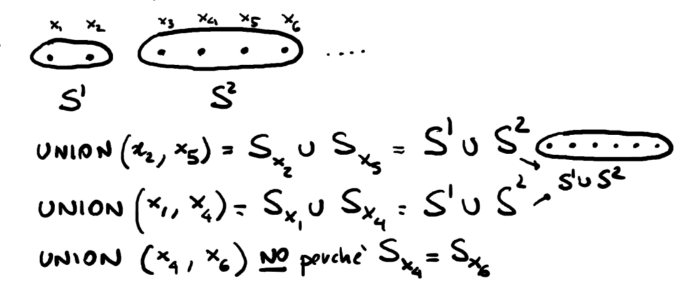
\includegraphics[scale=0.5]{Immagini/Screenshot From 2026-11-16 15-16-21.png}
\end{center}

Il rappresentante di $S_x \cup S_y$ può essere un elemento qualsiasi di $S_x \cup S_y$, di solito si mantiene il rappresentante di $S_x$ (o di $S_y$).

Dopo l'esecuzione di Union($x,y$) la collezione non conterrà più $S_x$ e $S_y$. Al loro posto ci sarà $S_x \cup S_y$

\subsubsection{Post condizioni}
\begin{itemize}
    \item L'esecuzione di una Union riduce di un'unità il numero di insiemi nella collezione $(K \to K-1)$
    \item Partendo da $\{\{x_1\}, \dots, \{x_n\}\}$ dopo $n-1$ Union la collezione diventa $\{X\}$, ossià un insieme contente la collezione di partenza, pertanto un algoritmo che utilizza una struttura dati per insiemi disgiunti \uline{esegue sempre al massimo $n-1$ Union}
\end{itemize}

\subsection{Find-Set: $X \to X$}

$\forall x \in X$, Find-Set($x$) = rapp($S_x$) dove rapp($S_x$) è il rappresentante di $S_x$.

Quindi dato $x \in X$ Find-Set($x$) è il rappresentante (attraverso un puntatore) dell'insieme $S_x$ al quale $x$ appartiene

\begin{center}
    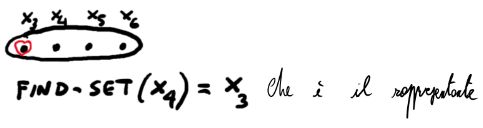
\includegraphics{Immagini/Find-Set.png}
\end{center}









        \usetikzlibrary{fit, calc, positioning, arrows.meta}
\usetikzlibrary{shapes.multipart, positioning, arrows.meta, calc}

\chapter{Rappresentazione di insiemi disgiunti mediante Liste Concatenate}
\section{Struttura della lista}
\begin{itemize}
    \item Ogni insieme è rappresentato mediante una lista
    \item Oggeto di un insieme (uno per ciascun insieme)
    \begin{itemize}
        \item \textbf{Head:} punta al 1° oggetto in lista
        \item \textbf{Tail:} punta all'ultimo oggetto in lista
    \end{itemize}

    \begin{figure}[htbp]
    \centering
        \begin{tikzpicture}[
            slot/.style={draw=black, semithick, minimum width=0.85cm, minimum height=0.35cm, inner sep=0pt},
            every node/.style={font=\normalsize}
        ]
            % Etichetta a sinistra
            \node (s_label) at (0, 0) {oggetto $S$};

            % Campi interni (head e tail)
            \node[anchor=west] (head_lbl) at (2.0, 0.35) {\texttt{head}};
            \node[slot, right=3mm of head_lbl] (head_ptr) {};

            \node[anchor=west] (tail_lbl) at (2.0, -0.35) {\texttt{tail}};
            \node[slot, right=3mm of tail_lbl] (tail_ptr) {};

            % Riquadro esterno dell'oggetto S
            \node[draw=black, thick, fit=(head_lbl) (head_ptr) (tail_lbl) (tail_ptr), inner xsep=6pt, inner ysep=5pt] (boxS) {};

            % Annotazioni a destra con incolonnamento delle virgolette
            \node[anchor=west, right=8mm of boxS.east] (desc) {
                \renewcommand{\arraystretch}{1.5}
                \begin{tabular}{@{}l l c c@{}}
                    puntatore & al $1^\circ$ & oggetto & in lista \\
                    \multicolumn{1}{c}{''} & all'ultimo & '' & ''
                \end{tabular}
            };
        \end{tikzpicture}
    \end{figure}

    \item Oggetto di una lista
    \begin{itemize}
        \item \textbf{set:} Puntatore all'oggetto dell'insieme
        \item \textbf{key:} Elemento dell'insieme
        \item \textbf{next:} Puntatore all'oggetto della lista dove contiene un altro elemento dell'insieme (oppure NIL)
    \end{itemize}

    \begin{figure}[htbp]
    \centering
    \begin{tikzpicture}[
        cell/.style={draw=black, thick, minimum width=2.2cm, minimum height=0.7cm, font=\ttfamily},
        every node/.style={font=\normalsize}
    ]
        % Riquadro dell'oggetto x (tre campi impilati)
        \node[cell] (set) {x.set};
        \node[cell, below=-\pgflinewidth of set] (key) {x.key};
        \node[cell, below=-\pgflinewidth of key] (next) {x.next};

        % Etichetta a sinistra (allineata al campo centrale)
        \node[left=1.2cm of key] (x_label) {oggetto $x$};

        % Annotazioni a destra
        \node[anchor=west, right=8mm of set] (desc_set) {puntatore all'oggetto dell'insieme};
        \node[anchor=west, right=8mm of key] (desc_key) {elemento dell'insieme};
        \node[anchor=west, right=8mm of next] (desc_next) {puntatore all'oggetto della lista};

        % Righe a capo per la descrizione di x.next perfettamente allineate
        \node[anchor=north west, align=left] at (desc_next.south west) {
            che contiene un altro elemento \\
            dell'insieme (oppure \texttt{NIL})
        };
    \end{tikzpicture}
    \end{figure}

    \item Il rappresentante è il 1° oggetto della lista
    

\end{itemize}

\begin{figure}[htbp]
\centering
% Definizione dell'insieme in alto
\noindent \underline{\textbf{ES:}} \quad $S^2 = \{c, h, e, b\}$

\vspace{0.8cm}

\begin{tikzpicture}[
    slot/.style={draw=black, semithick, minimum width=0.7cm, minimum height=0.32cm, inner sep=0pt},
    cell/.style={draw=black, semithick, minimum width=1.15cm, minimum height=0.48cm, font=\small},
    arr/.style={-{Stealth[length=2.2mm]}, thick},
    ptr/.style={circle, fill=black, inner sep=1.2pt}
]
    % --- 1. Riquadro Oggetto Insieme S^2 (a sinistra) ---
    \node[font=\bfseries\Large] (s2_lbl) at (-1.1, 0) {$S^2$};

    \node[anchor=west] (head_lbl) at (0, 0.32) {\texttt{head}};
    \node[slot, right=3mm of head_lbl] (head_slot) {};

    \node[anchor=west] (tail_lbl) at (0, -0.32) {\texttt{tail}};
    \node[slot, right=3mm of tail_lbl] (tail_slot) {};

    \node[draw=black, thick, fit=(head_lbl) (head_slot) (tail_lbl) (tail_slot), inner xsep=5pt, inner ysep=4pt] (boxS2) {};

    % --- 2. Elementi della lista concatenata (c, h, e, b) ---
    % Nodo 'c' (rappresentante)
    \node[cell, right=1.3cm of boxS2] (c_key) {$c$};
    \node[cell, above=-\pgflinewidth of c_key] (c_set) {};
    \node[cell, below=-\pgflinewidth of c_key] (c_next) {};
    \node[draw=black, thick, fit=(c_set) (c_next), inner sep=0pt] (box_c) {};

    % Nodo 'h'
    \node[cell, right=1.1cm of box_c.east |- c_key] (h_key) {$h$};
    \node[cell, above=-\pgflinewidth of h_key] (h_set) {};
    \node[cell, below=-\pgflinewidth of h_key] (h_next) {};
    \node[draw=black, thick, fit=(h_set) (h_next), inner sep=0pt] (box_h) {};

    % Nodo 'e'
    \node[cell, right=1.1cm of box_h.east |- h_key] (e_key) {$e$};
    \node[cell, above=-\pgflinewidth of e_key] (e_set) {};
    \node[cell, below=-\pgflinewidth of e_key] (e_next) {};
    \node[draw=black, thick, fit=(e_set) (e_next), inner sep=0pt] (box_e) {};

    % Nodo 'b' (ultimo elemento)
    \node[cell, right=1.1cm of box_e.east |- e_key] (b_key) {$b$};
    \node[cell, above=-\pgflinewidth of b_key] (b_set) {};
    \node[cell, below=-\pgflinewidth of b_key] (b_next) {};
    \node[draw=black, thick, fit=(b_set) (b_next), inner sep=0pt] (box_b) {};

    % --- 3. Punti di origine dei puntatori ---
    \node[ptr] (pt_head) at (head_slot.center) {};
    \node[ptr] (pt_tail) at (tail_slot.center) {};
    \node[ptr] (pt_c_set) at (c_set.center) {};
    \node[ptr] (pt_h_set) at (h_set.center) {};
    \node[ptr] (pt_e_set) at (e_set.center) {};
    \node[ptr] (pt_b_set) at (b_set.center) {};
    \node[ptr] (pt_c_next) at (c_next.center) {};
    \node[ptr] (pt_h_next) at (h_next.center) {};
    \node[ptr] (pt_e_next) at (e_next.center) {};

    % --- 4. Collegamenti head e next ---
    \draw[arr] (pt_head) -- (box_c.west |- c_key);
    \draw[arr] (pt_c_next) to[out=15, in=195] (box_h.west |- h_key);
    \draw[arr] (pt_h_next) to[out=15, in=195] (box_e.west |- e_key);
    \draw[arr] (pt_e_next) to[out=15, in=195] (box_b.west |- b_key);

    % Terminazione NIL per il nodo 'b'
    \draw[thick] (b_next.south west) -- (b_next.north east);
\node[below=4mm of b_next, font=\small\ttfamily] (nil) {NIL};    \draw[arr] (b_next.south) -- (nil.north);

    % --- 5. Puntatore tail (curva sotto tutti i blocchi) ---
    \draw[arr] (pt_tail) to[out=-25, in=-110, looseness=0.4] (box_b.south);

    % --- 6. Puntatori x.set (archi superiori verso S^2) ---
    \draw[arr] (pt_c_set) -- ++(0, 0.45) -| ([xshift=6mm]boxS2.north);
    \draw[arr] (pt_h_set) -- ++(0, 0.75) -| ([xshift=2mm]boxS2.north);
    \draw[arr] (pt_e_set) -- ++(0, 1.05) -| ([xshift=-2mm]boxS2.north);
    \draw[arr] (pt_b_set) -- ++(0, 1.35) -| ([xshift=-6mm]boxS2.north);

\end{tikzpicture}
\caption*{Rappresentazione con lista concatenata dell'insieme $S^2 = \{c, h, e, b\}$.}
\end{figure}

\newpage
\section{Metodi della lista}

\subsection{Make-Set}
Dato l'oggetto x si vuole creare una lista S avente x come unico oggetto

\begin{minipage}{0.45\textwidth}
    \begin{figure}[H]
        \centering
        \begin{tikzpicture}[
            slot/.style={draw=black, semithick, minimum width=0.75cm, minimum height=0.32cm, inner sep=0pt},
            cell/.style={draw=black, semithick, minimum width=1.4cm, minimum height=0.45cm, font=\small},
            arr/.style={-{Stealth[length=2.2mm]}, thick},
            ptr/.style={circle, fill=black, inner sep=1.1pt}
        ]
            % --- Oggetto Insieme S (a sinistra) ---
            \node[font=\bfseries\Large] (s_lbl) at (-0.9, 0) {$S$};

            \node[anchor=west] (head_lbl) at (0, 0.3) {\texttt{head}};
            \node[slot, right=3mm of head_lbl] (head_slot) {};

            \node[anchor=west] (tail_lbl) at (0, -0.3) {\texttt{tail}};
            \node[slot, right=3mm of tail_lbl] (tail_slot) {};

            \node[draw=black, thick, fit=(head_lbl) (head_slot) (tail_lbl) (tail_slot), inner xsep=5pt, inner ysep=4pt] (boxS) {};

            % --- Elemento x (a destra) ---
            \node[cell, right=1.6cm of boxS.east |- head_slot] (x_set) {};
            \node[cell, below=-\pgflinewidth of x_set] (x_key) {$x.key$};
            \node[cell, below=-\pgflinewidth of x_key] (x_next) {};
            \node[draw=black, thick, fit=(x_set) (x_next), inner sep=0pt] (box_x) {};

            % Tratto obliquo su next (rappresenta puntatore a NIL)
            \draw[thick] (x_next.south west) -- (x_next.north east);

            % Punti di origine dei puntatori
            \node[ptr] (pt_head) at (head_slot.center) {};
            \node[ptr] (pt_tail) at (tail_slot.center) {};
            \node[ptr] (pt_set) at (x_set.center) {};

            % Frecce da head e tail verso l'oggetto x
            \draw[arr] (pt_head) -- (box_x.west |- x_set);
            \draw[arr] (pt_tail) -- (box_x.west |- x_next);

            % Freccia x.set di ritorno verso l'oggetto insieme S
            \draw[arr] (pt_set) to[out=110, in=70, looseness=1.2] (boxS.north);

            % Puntatore della variabile x dal basso verso il blocco
            \node (x_var) at ([shift={(-0.6cm, -1.0cm)}]box_x.south) {$x$};
            \draw[arr] (x_var) -- (box_x.south);

            % Rappresentazione dell'insieme a destra
            \node[right=0.8cm of box_x.east, font=\large] (set_repr) {$\{x.key\}$};

            % Costo temporale in basso
            \node[anchor=north west, align=left, font=\normalsize] (cost) at ([yshift=-1.2cm]boxS.south west) {
                \textbf{COSTO} \\
                \small (in tempo)
            };
            \node[right=2mm of cost.mid east, font=\large] (cost_val) {$: \; O(1)$};

        \end{tikzpicture}
    \end{figure}
\end{minipage}
\hfill
\begin{minipage}{0.45\textwidth}
    \begin{algorithmic}
        \Procedure{MAKE-SET}{x}
            \State new S
            \State S.head = x
            \State S.tail = x
            \State x.set = S
            \State x.next = NIL
        \EndProcedure
    \end{algorithmic}
\end{minipage}

\subsection{Find-Set}

\begin{center}
    \begin{algorithmic}
        \Procedure{FIND-SET}{x}
        \State \Return x.set.head
        \EndProcedure
    \end{algorithmic}
\end{center}

\begin{figure}[H]
\centering
\begin{tikzpicture}[
    slot/.style={draw=black, semithick, minimum width=0.75cm, minimum height=0.32cm, inner sep=0pt},
    cell/.style={draw=black, semithick, minimum width=1.15cm, minimum height=0.42cm, font=\small},
    arr/.style={-{Stealth[length=2.2mm]}, thick},
    ptr/.style={circle, fill=black, inner sep=1.1pt}
]
    % --- 1. Oggetto Insieme S (a sinistra) ---
    \node[font=\bfseries\Large] (s_lbl) at (-0.9, 0) {$S$};

    \node[anchor=west] (head_lbl) at (0, 0.3) {\texttt{head}};
    \node[slot, right=3mm of head_lbl] (head_slot) {};

    \node[anchor=west] (tail_lbl) at (0, -0.3) {\texttt{tail}};
    \node[slot, right=3mm of tail_lbl] (tail_slot) {};

    \node[draw=black, thick, fit=(head_lbl) (head_slot) (tail_lbl) (tail_slot), inner xsep=5pt, inner ysep=4pt] (boxS) {};

    % --- 2. Elementi della lista concatenata ---
    % Blocco 1 (testa)
    \node[cell, right=1.2cm of boxS.east |- head_slot] (b1_set) {};
    \node[cell, below=-\pgflinewidth of b1_set] (b1_key) {};
    \node[cell, below=-\pgflinewidth of b1_key] (b1_next) {};
    \node[draw=black, thick, fit=(b1_set) (b1_next), inner sep=0pt] (box_b1) {};

    % Blocco 2
    \node[cell, right=1.0cm of box_b1.east |- b1_set] (b2_set) {};
    \node[cell, below=-\pgflinewidth of b2_set] (b2_key) {};
    \node[cell, below=-\pgflinewidth of b2_key] (b2_next) {};
    \node[draw=black, thick, fit=(b2_set) (b2_next), inner sep=0pt] (box_b2) {};

    % Primi puntini di sospensione
    \node[right=3mm of box_b2.east |- b1_key, font=\large] (dots1) {$\dots$};

    % Blocco x
    \node[cell, right=3mm of dots1.east |- b1_set] (bx_set) {};
    \node[cell, below=-\pgflinewidth of bx_set] (bx_key) {};
    \node[cell, below=-\pgflinewidth of bx_key] (bx_next) {};
    \node[draw=black, thick, fit=(bx_set) (bx_next), inner sep=0pt] (box_bx) {};

    % Secondi puntini di sospensione
    \node[right=3mm of box_bx.east |- b1_key, font=\large] (dots2) {$\dots$};

    % Ultimo blocco (coda)
    \node[cell, right=3mm of dots2.east |- b1_set] (blast_set) {};
    \node[cell, below=-\pgflinewidth of blast_set] (blast_key) {};
    \node[cell, below=-\pgflinewidth of blast_key] (blast_next) {};
    \node[draw=black, thick, fit=(blast_set) (blast_next), inner sep=0pt] (box_blast) {};

    % Slash per puntatore NIL nell'ultimo blocco
    \draw[thick] (blast_next.south west) -- (blast_next.north east);

    % --- 3. Punti di origine dei puntatori ---
    \node[ptr] (pt_head) at (head_slot.center) {};
    \node[ptr] (pt_b1_set) at (b1_set.center) {};
    \node[ptr] (pt_b2_set) at (b2_set.center) {};
    \node[ptr] (pt_bx_set) at (bx_set.center) {};
    \node[ptr] (pt_blast_set) at (blast_set.center) {};
    \node[ptr] (pt_b1_next) at (b1_next.center) {};
    \node[ptr] (pt_b2_next) at (b2_next.center) {};
    \node[ptr] (pt_bx_next) at (bx_next.center) {};

    % --- 4. Collegamenti orizzontali (head e next) ---
    \draw[arr] (pt_head) -- (box_b1.west |- b1_set);
    \draw[arr] (pt_b1_next) to[out=15, in=195] (box_b2.west |- b2_key);
    \draw[arr] (pt_b2_next) -- (dots1.west);
    \draw[arr] (pt_bx_next) -- (dots2.west);

    % --- 5. Variabile x puntata dal basso verso il blocco x ---
    \node (x_var) at ([shift={(-0.6cm, -1.0cm)}]box_bx.south) {$x$};
    \draw[arr] (x_var) -- (box_bx.south);

    % --- 6. Puntatori di ritorno verso l'oggetto S (operazione Find-Set) ---
    \draw[arr] (pt_b1_set) -- ++(0, 0.45) -| ([xshift=6mm]boxS.north);
    \draw[arr] (pt_b2_set) -- ++(0, 0.75) -| ([xshift=2mm]boxS.north);
    \draw[arr] (pt_bx_set) -- ++(0, 1.05) -| ([xshift=-2mm]boxS.north);
    \draw[arr] (pt_blast_set) -- ++(0, 1.35) -| ([xshift=-6mm]boxS.north);

    % Etichetta "return S"
    \node[anchor=south west, font=\small\ttfamily] at ([yshift=1.1cm]boxS.north west) {return $S$};

\end{tikzpicture}
\caption{Funzionamento dell'operazione \textsc{Find-Set}($x$) in tempo $O(1)$ tramite puntatore diretto all'oggetto insieme $S$.}
\end{figure}

\newpage
\subsection{Union}
La più semplice implementazione dell'operazione Union che usa la rappresentazione degli insiemi mediante liste concatenate richiede molto più tempo rispetto all'operazione Make-Set o Find-Set.

\begin{tikzpicture}[
    >=Stealth,
    font=\small,
    % Stile per i nodi della lista (3 campi verticali)
    listnode/.style={
        rectangle split,
        rectangle split parts=3,
        draw,
        fill=gray!12,
        minimum width=1.1cm,
        rectangle split part fill={gray!12, white, gray!12},
        inner sep=4pt
    },
    % Stile per l'intestazione dell'insieme
    setheader/.style={
        draw,
        fill=gray!45,
        minimum width=1.9cm,
        minimum height=2.4cm,
        inner sep=0pt
    },
    % Puntatori interni (quadratini bianchi)
    ptmbox/.style={
        draw,
        fill=white,
        minimum size=0.45cm,
        inner sep=0pt
    }
]


    % Blocco Insieme (Header)
    \node[setheader] (S) at (0, 0) {};
    \node[left=2pt of S.west] {$S_1$};

    % Testo ed elementi interni all'Header
    \node[anchor=west] at ([xshift=3pt, yshift=0.45cm]S.west) {\textit{head}};
    \node[ptmbox] (head_box) at ([xshift=-0.4cm, yshift=0.45cm]S.east) {};

    \node[anchor=west] at ([xshift=3pt, yshift=-0.55cm]S.west) {\textit{tail}};
    \node[ptmbox] (tail_box) at ([xshift=-0.4cm, yshift=-0.55cm]S.east) {};

    % Nodi della lista concatenata
    \node[listnode] (N1) at (2.4, 0.45) {\nodepart{two}$f$\nodepart{three}\phantom{/}};
    \node[listnode] (N2) at (4.3, 0.45) {\nodepart{two}$g$\nodepart{three}\phantom{/}};
    \node[listnode] (N3) at (6.2, 0.45) {\nodepart{two}$d$\nodepart{three}\phantom{/}};
    \node[listnode] (N4) at (8.1, 0.45) {\nodepart{two}$c$\nodepart{three}\phantom{/}};
    \node[listnode] (N5) at (10.0, 0.45) {\nodepart{two}$h$\nodepart{three}\phantom{/}};
    \node[listnode] (N6) at (11.9, 0.45) {\nodepart{two}$e$\nodepart{three}\phantom{/}};
    \node[listnode] (N7) at (13.8, 0.45) {\nodepart{two}$b$\nodepart{three}/};

    % Puntatore head -> primo elemento
    \draw[->] (head_box.center) -- (N1.text split west);

    % Puntatori next tra elementi consecutivi
    \foreach \i/\j in {1/2, 2/3, 3/4, 4/5, 5/6, 6/7} {
        \draw[->] (N\i.three split) -- (N\j.three split west);
    }

    % Puntatore tail -> ultimo elemento
    \draw[->] (tail_box.center) -- ++(12.85, 0) -- (N7.south);

    % Puntatori dai campi superiori dei nodi verso la testa dell'insieme S1
    % Ogni linea ha una quota orizzontale progressiva e un punto di arrivo distinto sulla testa di S
    \foreach \i/\h/\xoffset in {
        1/1.95/0.85,
        2/2.15/0.70,
        3/2.35/0.55,
        4/2.55/0.40,
        5/2.75/0.25,
        6/2.95/0.10,
        7/3.15/-0.05
    } {
        \draw[->] (N\i.north) 
            -- ++(0, \h - 0.45) 
            -- ([xshift=\xoffset cm]S.north |- 0, \h + 1.05) 
            -- ([xshift=\xoffset cm]S.north);
    }

\end{tikzpicture}



Eseguiamo la Union(x,y) aggiungendo la lista y alla fine della lista .

Il rappresentante della lista x diventa il rappresentante della lista finale. 

Purtroppo dobbiamo aggiornare il puntatore all'oggetto dell'insieme per ogni oggetto che originariamente si trovava nella lista, questo richiede un tempo lineare nella lunghezza della lista y.

Eseguiamo $n$ operazioni Make-Set, seguite da $n-1$ operazioni Union, quindi $m=2n-1$. 
Impieghiamo un tempo $\Theta(n)$ per eseguire le $n$ operazioni Make-Set. Poichè l'i-esima operazione Union aggiorna $i$ oggetti, il numero totale di oggetti aggiornati da tutte le $n-1$ operazioni Union è

{
    \Large
    \[
        \sum^{n-1}_{i=1} i = \mathbf{\Theta(n^2)}
    \]
}

\begin{center}
    \begin{algorithmic}[1]
        \Procedure{Union}{$x, y$}
            \State $S_1 \gets x.set$
            \State $S_2 \gets y.set$
            \State $S_1.tail.next \gets S_2.head$
            \State $S_1.tail \gets S_2.tail$
            \State $z \gets S_2.head$
            \While{$z \neq \text{NIL}$}
                \State $z.set \gets S_1$
                \State $z \gets z.next$
            \EndWhile
            \State \Return $S_1$
        \EndProcedure
    \end{algorithmic}
\end{center}

\newpage
\section{Euristica dell'unione pesata}
Nel caso peggiore, l'implementazione dell'operazione UNION richiede un tempo medio $\Theta(n)$ per chiamata, perchè potremmo appendere una lista più lunga a una più corta, dobbiamo aggiornare il puntatore all'oggetto dell'insieme per ogni elemento della lista più lunga.

Supponiamo invece che:
\begin{itemize}
    \item Ogni lista includa anche la sua lunghezza
    \item Appendiamo ogni volta la lista più corta a quella più lunga, risolvendo in modo arbitrario i casi di liste aventi la stessa lunghezza
\end{itemize}

Con questa \textbf{euristica dell'unione pesata}, una singola operazione UNION può ancora impiegare $\Omega(n)$ se entrambe le liste hanno $\Omega(n)$ elementi.

Tuttavia, una sequenza di $m$ operazioni Make-Set,Union e Find-Setn $n$ delle quali sono perazioni Make-Set, impiega un tempo $O(m+n\log(n))$

\subsection{Teorema}
Utilizzando la rappresentazione degli insiemi disgiunti tramite liste concatenate e l'euristica dell'unione pesata, una sequenza di $m$ operazioni Make-Set, Union e Find-Set, $n$ delle quali sono operazioni Make-Set, impiega un tempo $O(m+n\log(n))$

\subsection{Dimostrazione}
Sia $x$ un qualunque oggetto (ce ne sono $n$) calcoliamo il massimo numero di volte che x.set viene aggiornato. Ogni volta che x.set viene aggiornato x si deve trovare nella lista più corta

\begin{table}[htbp]
\centering
\renewcommand{\arraystretch}{1.5}
    \begin{tabular}{lll}
    $1^{\text{a}}$ volta che \texttt{x.set} viene aggiornato & l'insieme risultante ha almeno & $2$ elementi \\
    $2^{\text{a}}$ volta che \texttt{x.set} viene aggiornato  & l'insieme risultante ha almeno & $2^2$ elementi \\
    \hspace{2.3em} $\vdots$ & & \\
    $i\text{-ma}$ volta che \texttt{x.set} viene aggiornato & l'insieme risultante ha almeno & $2^i$ elementi
    \end{tabular}
\end{table}

Quindi x.set è aggiornato al massimo $\log(n)$ volte. Questo perchè se fosse aggiornato più di $\log(n)$ volte l'insieme risultante avrebbe \textbf{almeno}

$$
    2^{\log(n)} > n \text{ elementi} \implies \text{Impossibile}
$$

Siccome ci sono $n$ oggetti il costo è $\mathbf{O(n+n\log(n))}$

\subsection{Algoritmo}
\begin{algorithmic}[1]
\Procedure{Union}{$x, y$}
    \State $S_1 \gets x.\textit{set}$
    \State $S_2 \gets y.\textit{set}$
    \If{$S_1 == S_2$}
        \State \Return $S_1$
    \EndIf
    \If{$S_1.\textit{length} \ge S_2.\textit{length}$}
        \State $S_1.\textit{tail}.\textit{next} \gets S_2.\textit{head}$
        \State $S_1.\textit{tail} \gets S_2.\textit{tail}$
        \State $z \gets S_2.\textit{head}$
        \While{$z \neq \text{NIL}$}
            \State $z.\textit{set} \gets S_1$
            \State $z \gets z.\textit{next}$
        \EndWhile
        \State $S_1.\textit{length} \gets S_1.\textit{length} + S_2.\textit{length}$
        \State \Return $S_1$
    \Else
        \State $S_2.\textit{tail}.\textit{next} \gets S_1.\textit{head}$
        \State $S_2.\textit{tail} \gets S_1.\textit{tail}$
        \State $z \gets S_1.\textit{head}$
        \While{$z \neq \text{NIL}$}
            \State $z.\textit{set} \gets S_2$
            \State $z \gets z.\textit{next}$
        \EndWhile
        \State $S_2.\textit{length} \gets S_2.\textit{length} + S_1.\textit{length}$
        \State \Return $S_2$
    \EndIf
\EndProcedure
\end{algorithmic}
        \chapter{Rappresentazione di insiemi disgiunti mediante Foreste di insiemi Disgiunti}

\section{Struttura della foresta}
In una rappresentazione più veloce degli insiemi disgiunti, rappresentiamo gli insiemi con alberi radicati, dove:
\begin{itemize}
    \item Ogni insieme è rappresentato da un albero radicato
    \item Ogni nodo contiene un elemento
    \item Ogni nodo punta al padre e la radice a se stessa
    \item La radice contiene il rappresentante
\end{itemize}

\subsection{Esempio grafico}
\begin{figure}[htbp]
\centering
\begin{tikzpicture}[
    vertex/.style={
        circle,
        draw=black!75,
        fill=black!7,
        inner sep=0pt,
        minimum size=8mm,
        font=\large\itshape,
        line width=0.6pt
    },
    edge/.style={
        -{Stealth[length=2.8mm, width=2.1mm]},
        line width=0.85pt,
        draw=black!90,
        shorten >=1pt,
        shorten <=1pt
    },
    loop edge/.style={
        -{Stealth[length=2.8mm, width=2.1mm]},
        line width=0.85pt,
        draw=black!90,
        looseness=6,
        in=125,
        out=55
    },
    sublabel/.style={
        font=\large,
        text=black
    }
]

% ==================== PARTE (a) ====================
\begin{scope}[xshift=0cm]
    % Albero con radice c
    \node[vertex] (c) at (2.2, 4.0) {$c$};
    \node[vertex] (h) at (1.0, 2.3) {$h$};
    \node[vertex] (e) at (3.4, 2.3) {$e$};
    \node[vertex] (b) at (1.0, 0.6) {$b$};

    % Albero con radice f
    \node[vertex] (f1) at (6.2, 4.0) {$f$};
    \node[vertex] (d1) at (6.2, 2.3) {$d$};
    \node[vertex] (g1) at (6.2, 0.6) {$g$};

    % Archi albero c
    \draw[edge] (h) -- (c);
    \draw[edge] (e) -- (c);
    \draw[edge] (b) -- (h);
    \draw[loop edge] (c) to (c);

    % Archi albero f
    \draw[edge] (d1) -- (f1);
    \draw[edge] (g1) -- (d1);
    \draw[loop edge] (f1) to (f1);

    % Etichetta (a)
    \node[sublabel] at (3.9, -1.8) {(a)};
\end{scope}

% ==================== PARTE (b) ====================
\begin{scope}[xshift=10.5cm]
    % Radice f
    \node[vertex] (f2) at (3.0, 4.0) {$f$};

    % Figli di f
    \node[vertex] (c2) at (1.4, 2.3) {$c$};
    \node[vertex] (d2) at (4.6, 2.3) {$d$};

    % Figli di c e d
    \node[vertex] (h2) at (0.2, 0.6) {$h$};
    \node[vertex] (e2) at (2.6, 0.6) {$e$};
    \node[vertex] (g2) at (4.6, 0.6) {$g$};

    % Figlio di h
    \node[vertex] (b2) at (0.2, -1.1) {$b$};

    % Archi
    \draw[edge] (c2) -- (f2);
    \draw[edge] (d2) -- (f2);
    \draw[edge] (h2) -- (c2);
    \draw[edge] (e2) -- (c2);
    \draw[edge] (g2) -- (d2);
    \draw[edge] (b2) -- (h2);
    \draw[loop edge] (f2) to (f2);

    % Etichetta (b)
    \node[sublabel] at (3.0, -1.8) {(b)};
\end{scope}

\end{tikzpicture}
\end{figure}

\section{Pseudocodice Metodi Stock}


\subsection{Make-Set}
\begin{algorithmic}
    \Procedure{Make-Set}{$x$}
        \State $x.p = x$
    \EndProcedure
\end{algorithmic}

\subsection{Find-Set}
\begin{algorithmic}
    \Procedure{Find-Set}{$x$}
        \If{$x.p = x$}
            \State \Return $x.p$

            \Else
                \State \Return \Call{Find-Set}{$x.p$}
        \EndIf
    \EndProcedure
\end{algorithmic}


\subsection{Union}
La radice di un albero punta la radice dell'altro

\begin{algorithmic}
    \Procedure{Union}{x,y}
        \State $z = \Call{Find-Set}{$x$}$
        \State $w = \Call{Find-Set}{y}$
        \State $z.p = w$
    \EndProcedure
\end{algorithmic}

Una sequenza di $n-1$ Union può creare una catena lineare di $n$ nodi

\begin{figure}[htbp]
\centering
\begin{tikzpicture}[
    vertex/.style={
        circle,
        draw=black,
        line width=1.3pt,
        minimum size=8.5mm,
        inner sep=0pt,
        font=\large\bfseries
    },
    arrow edge/.style={
        -{Stealth[length=3mm, width=2.2mm]},
        line width=1.3pt,
        draw=black,
        shorten <=2pt,
        shorten >=2pt
    },
    loop edge/.style={
        -{Stealth[length=3mm, width=2.2mm]},
        line width=1.3pt,
        draw=black,
        looseness=6,
        in=100,
        out=25
    },
    op label/.style={
        anchor=west,
        font=\large\bfseries
    }
]

    % Parametri di spaziatura
    % x: a=0, b=2.2, c=4.4, d=6.6
    % y: Riga 1 = 0, Riga 2 = -2.2, Riga 3 = -4.4, Riga 4 = -6.6

    % ==================== RIGA 1 (Stato Iniziale) ====================
    \node[vertex] (a1) at (0, 0) {a};
    \node[vertex] (b1) at (2.2, 0) {b};
    \node[vertex] (c1) at (4.4, 0) {c};
    \node[vertex] (d1) at (6.6, 0) {d};

    \draw[loop edge] (a1) to (a1);
    \draw[loop edge] (b1) to (b1);
    \draw[loop edge] (c1) to (c1);
    \draw[loop edge] (d1) to (d1);

    \node[anchor=west, font=\LARGE\bfseries] at (8.0, 0) {$n=4$};

    % ==================== RIGA 2: UNION(a, b) ====================
    \node[op label] at (-0.6, -1.3) {\textsc{Union}\,(a, b)};

    \node[vertex] (a2) at (0, -2.2) {a};
    \node[vertex] (b2) at (2.2, -2.2) {b};
    \node[vertex] (c2) at (4.4, -2.2) {c};
    \node[vertex] (d2) at (6.6, -2.2) {d};

    \draw[arrow edge] (a2) -- (b2);
    \draw[loop edge] (b2) to (b2);
    \draw[loop edge] (c2) to (c2);
    \draw[loop edge] (d2) to (d2);

    % ==================== RIGA 3: UNION(a, c) ====================
    \node[op label] at (-0.6, -3.5) {\textsc{Union}\,(a, c)};

    \node[vertex] (a3) at (0, -4.4) {a};
    \node[vertex] (b3) at (2.2, -4.4) {b};
    \node[vertex] (c3) at (4.4, -4.4) {c};
    \node[vertex] (d3) at (6.6, -4.4) {d};

    \draw[arrow edge] (a3) -- (b3);
    \draw[arrow edge] (b3) -- (c3);
    \draw[loop edge] (c3) to (c3);
    \draw[loop edge] (d3) to (d3);

    % ==================== RIGA 4: UNION(a, d) ====================
    \node[op label] at (-0.6, -5.7) {\textsc{Union}\,(a, d)};

    \node[vertex] (a4) at (0, -6.6) {a};
    \node[vertex] (b4) at (2.2, -6.6) {b};
    \node[vertex] (c4) at (4.4, -6.6) {c};
    \node[vertex] (d4) at (6.6, -6.6) {d};

    \draw[arrow edge] (a4) -- (b4);
    \draw[arrow edge] (b4) -- (c4);
    \draw[arrow edge] (c4) -- (d4);
    \draw[loop edge] (d4) to (d4);

\end{tikzpicture}
\end{figure}

\newpage
\section{Euristica dell'unione per rango + compressione dei cammini}
\begin{itemize}
    \item \textbf{Altezza di un nodo $\mathbf{x}$}: Numero di archi su un più lungo cammino da $x$ ad una foglia
    \item \textbf{Rango di un nodo $\mathbf{x}$}: Limite superiore dell'altezza di $x$
\end{itemize}

\subsection{Unione per rango}
La radice di rango <punta a quella di rango>.

In tal modo il rango della radice dell'albero così ottenuto non aumenta rispetto al rango, a meno che i ranghi non siano uguali ed in tal caso aumenta di 1.

\subsection{Metodi}

\subsubsection{Make-Set}
\begin{algorithmic}
    \Procedure{Make-Set}{$x$}
        \State $x.p = x$
        \State $x.rank = 0$
    \EndProcedure
\end{algorithmic}

\subsubsection{Union}
\begin{algorithmic}
    \Procedure{Union}{$x,y$}
        \State \Call{Link}{\Call{Find-Set}{$x$},\Call{Find-Set}{$y$}}
    \EndProcedure
\end{algorithmic}

\subsubsection{Link}
\begin{algorithmic}
    \Procedure{Link}{$x,y$}
        \If{$x.rank > y.rank$}
            \State $y.p = x$

            \Else
                \State $x.p = y$

                    \If{$x.rank = y.rank$}
                        \State $y.rank = y.rank + 1$
                    \EndIf
        \EndIf
    \EndProcedure
\end{algorithmic}

\subsubsection{Find-Set con compressione dei cammini}
\begin{algorithmic}
    \Procedure{Find-Set}{$x$}
        \If{$x.p \not = x$}
            \State $x.p = \Call{Find-Set}{$x.p$}$
        \EndIf

        \State \Return $x.p$
    \EndProcedure
\end{algorithmic}






        \chapter{Greedy-Max}
\section{Procedimento Greedy}

\subsection{Problema}
\begin{center}
    Consideriamo la seguente istanza di Knapsack-01
\end{center}

\begin{minipage}[t]{0.55\textwidth}
    \centering
    \begin{tabular}{ccc}
        \textbf{OGGETTO} & \textbf{VALORE} & \textbf{INGOMBRO} \\
        \midrule
        $x_1$ & 100 & 30 \\
        $x_2$ & 80  & 25 \\
        $x_3$ & 60  & 20 \\
    \end{tabular}
\end{minipage}
\hfill
\begin{minipage}[t]{0.4\textwidth}
    \textbf{CAPACITÀ ZAINO:}
    \vspace{0.5em}
    
    $C = 45$
\end{minipage}

\vspace{2em}

\noindent \textbf{SOLUZIONE:} \quad $S = \{x_2, x_3\}$

La soluzione si trova utilizzando la programmazione Dinamica

\subsection{Procedimento algoritmo Greedy}
\begin{enumerate}
    \item Si effettua una scelta (quella greedy)
    \item Si risolve un sottoproblema
\end{enumerate}

In un algoritmo greedy facciamo la scelta che sembra migliore in un determinato momento e poi risolviamo il problema che deriva da tale scelta.

La scelta di un algoritmo goloso può dipendere dalle precedenti scelte ma non può dipendere dalle scelte future o dalle soluzioni dei sottoproblemi.

\subsection{Soluzione ottenuta attraverso Greedy}
Nel caso presentato:
\begin{enumerate}
    \item Includo $x_1$ nella soluzione
    \item Il sottoproblema da risolvere sarà $\{x_2, x_3\}$ con capacità residua $= 15$
    \item La soluzione del sottoproblema è $\emptyset$
\end{enumerate}

Applicando la tecnica greedy si ottiene l'insieme $\{x_1\} \cup \emptyset$ \uline{che però non è la soluzione ottimale}.


La tecnica greedy non porta sempre a trovare la soluzione ottima, vale la pena capire quando è percorribile perchè permette di ottenere algoritmi semplici e di facile implementazione

\section{Confronto  tra Programmazione Dinamica e Tecnica Greedy}

\begin{minipage}[t]{0.47\textwidth}
  % Linea orizzontale superiore sinistra
  \rule{\linewidth}{1.2pt}\\[0.8em]
  
  \centering
  {PROGRAMMAZIONE DINAMICA}\\[1.4em]
  
  \raggedright
  Le decisioni vengono prese in base alla risoluzione dei sottoproblemi.\\[1.4em]
  
  \begin{enumerate}
    \item Si risolvono i sottoproblemi
    \item Si effettua una scelta
  \end{enumerate}

  \vspace{1.8em}
  \begin{center}
    \textbf{BOTTOM-UP}
  \end{center}
\end{minipage}%
\hfill
% Linea verticale divisoria
\vrule width 1.2pt
\hfill
\begin{minipage}[t]{0.47\textwidth}
  % Linea orizzontale superiore destra
  \rule{\linewidth}{1.2pt}\\[0.8em]
  
  \centering
  PROGRAMMAZIONE GREEDY\\[1.4em]
  
  \raggedright
  Viene presa la decisione che al momento appare la migliore e poi si risolve un sottopb.\\[1.4em]
  
  \begin{enumerate}
    \item Si effettua una scelta
    \item Si risolve \underline{\textbf{UN}} sottoproblema
  \end{enumerate}

  \vspace{1.8em}
    \begin{center}
        \textbf{SOLITAMENTE TOP-DOWN}    
    \end{center}
\end{minipage}

In entrambe le tecniche vale la proprietà della sottostruttura ottima-

Per capire quando la tecnica Greedy funziona occorre introdurre alcuni concetti.

\section{Sistema Indipendenza (S.I)}

\subsection{Definizione}

Un sistema di indipendenza è una coppia $<E,F>$ dove:

\begin{itemize}
    \item $E$ è un insieme finito ($|E| < \infty$)
    \item $F$ è una famiglia di sottoinsiemi di $E\ (F \subseteq \mathcal{P}(E))$ tali che:
    {
        \large
        $$
        \forall A \in F, \forall B \subseteq A \text{ vale che } B \in F
        $$
    }
\end{itemize}

\subsection{Esempio 1}
$$\langle E,F \rangle$$

\begin{itemize}
    \item $E$ è un insieme finito qualunque
    \item $F = \mathcal{P}(E)$
\end{itemize}

\begin{center}
    È un sistema di indipendenza
\end{center}

\subsection{Esempio 2}
$$
    \langle E,F \rangle
$$

\begin{itemize}
    \item $E \subseteq V$ con $V$ spazio vettoriale e $|E| < \infty$
    \item $F = \{A \subseteq E : A \text{ è un insieme di vettori linearmente indipendenti}\}$
\end{itemize}

\begin{center}
    È un sistema di indipendenza
\end{center}

\newpage
\subsection{Esempio 3}
$$
G = (V,E) \text{un grafo non orientato}
$$

\begin{itemize}
    \item $\langle E,F \rangle$ con $F = \{A \subseteq E : (V,A) \text{ è una foresta}\}$
\end{itemize}

\begin{center}
    È un sistema di indipendenza
\end{center}

Infatti, scelto $A \subseteq F$ (quindi $(V,A)$ è una foresta) e scelto $B \subseteq A$ si ha che $(V,B)$ è una foresta, per cui $B \in F$


\section{Insieme Massimale (Non estendibile)}

\subsection{Definizione}

$A \in F$ è massimale se e solo se $A \in E \backslash A$ vale che $A \cup \{e\} \not \in F$

\section{Problema di massimo associato ad un S.I}

\subsection{Istanza}
\begin{itemize}
    \item $\langle E,F \rangle$ è un sistema di indipendenza
    \item $w: E \to R$
\end{itemize}

\subsection{Soluzione}
{
    \large 
    

    $$
    M \in F \text{ massimale tale che }
    w(M) = \max_{\substack{A \in F \text{ con } A \text{ massiale}}}\{w(A)\}
    $$
}

\subsection{Esempio 4}
\begin{itemize}
    \item $E = \{x_1 , \dots, x_m\}$ e $\forall x_i$ ha un ingombro $ing(x_i)$
    \item $F = \{A \subseteq E : ing(A) \leq C\}$
    \item $w : E \to R^+ \quad \forall x_i\ w(x_i)$ è il valore di $x_i$
\end{itemize}

\subsubsection{Nota}

$\langle E,F \rangle$ è un S.I se:
\begin{itemize}
    \item $A \in F,\ ing(A) \leq C$
    \item $B \subseteq A$
    \item $ing(B) \leq ing(a) \leq C \implies B \in F$
\end{itemize}

Inoltre il problema con 
\begin{itemize}
    \item \textbf{Istanza}: $\langle E,F \rangle \text{ e } w$
    \item \textbf{Soluzione}: $M \in F$ massimale tale che $w(M) = \max_{\substack{A \in F \text{ con } A \text{ massiale}}}\{w(A)\}$
\end{itemize}
è il Knapsack-01

\newpage
\section{Algoritmo Greedy Associato ad un S.I $\langle E,F \rangle$ e $w:E \to R^+$}

\subsection{Pseudocodice}
\begin{algorithmic}
    \Procedure{Greedy-Max}{$E,F,w$} \Comment{$E = \{e_1 , \dots, e_n\}$}
        \State $S = \emptyset$
        \State $Q = [1, \dots, m] = (e_1, \dots, e_m)$
        \State $Q = Sort(Q)$ \Comment{Ordinamente decrescente in baso ai pesi}

        \For{$i = 1$ to $n$}
            \If{$S \cup \{Q[i]\} \in F$} \Comment{Costo: $O(n\log(n)+ n \cdot C(n))$}
                \State $S = S \cup \{Q[i]\}$
            \EndIf
        \EndFor

        \State \Return $S$
    \EndProcedure
\end{algorithmic}

\subsection{Cosa restituisce?}
Greedy-Max ritorna sempre un  sottoinsieme massimale

\subsection{Quando Greedy-Max risolve il problema?}
Greedy-Max risolve i problemi associati a dei \textbf{matroidi}, la cui teoria è utile per determinare quando il metodo greedy genera solozuini ottime, essa non tratta tutti i casi ai quali è possibile applicare il metodo greedy ma consente di analizzare molti casi di interesse pratico
        \usetikzlibrary{shapes, backgrounds}

\chapter{Matroidi}

\section{Definizione}
Un Sistema di Indipendenza $\langle E,F \rangle$ è un matroide se e solo se vale la seguente proprietà (detto "di scambio")

{
    \large
    $$
    \forall A,B \in F \text{ con } |B| > |A| \quad \exists b \in B \backslash A \text{ tale che } A \cup \{b\} \in F
    $$

    $$
    |B| > |A| \text{ si può sostituire equivalentemente con } |B| = |A|+1 
    $$
}

\subsection{Esempi di matroidi}
\begin{itemize}
    \item Il S.I $\langle E, \mathcal{P}(E) \rangle$ dell'esempio 1 è un matroide
    \item Il S.I dell'esempio 2 è un matroide
    \item Il S.I dell'esempio 3 (matroide grafico) è un matroide
    \item Il S.I dell'esempio 4 non è un matroide
    $$
    \begin{aligned}
        A = \{x_1\} \in F & \quad (\text{ing}(A) = 30 \leq 45) \\
        B = \{x_2, x_3\} \in F & \quad (\text{ing(B)} = 45 \leq 45) \\
        \not \exists b \in B \backslash A : A \cup \{b\} \in F & \quad \text{Non rispetta la proprietà di scambio } \\ 
    \end{aligned}
    $$
    \begin{center}
        Infatti $ing(A \cup b) > 45$ con $b \in B \backslash A$
    \end{center}
\end{itemize}

\section{Teorema della dimensione di un matroide}

\subsection{Proposizione}
Sia $\langle E,F \rangle$ un matroide, tutti gli insiemi massimali di $\langle E,F \rangle$ hanno la stessa cardinalità

\subsection{Dimostrazione}
Per assurdo, siano $A,B \in F$ massimali con $|B| > |A|$ per la proprietà dello scambio 

$$
\exists b \in B \backslash A : A \cup \{b\} \in F
$$

quindi $A$ è estendibile, il che è una contraddizione

\newpage
\section{Matroidi grafici}

\subsection{Obiettivo}
Vogliamo ora far vedere che il matroide grafico è un matroide.

\begin{itemize}
    \item Sia $G = (V,E)$ un grafo orientato
    \item Sia $\langle E,F \rangle$ il S.I con $F=\{A \subseteq E : (V,A) \text{ è una foresta}\}$
\end{itemize}

\begin{figure}[htbp]
\centering
\definecolor{highlightpink}{RGB}{255, 204, 218}
\definecolor{softpurple}{RGB}{220, 210, 245}
\definecolor{softblue}{RGB}{210, 220, 250}

\begin{tikzpicture}[
    vertex/.style={circle, draw, thick, inner sep=0pt, minimum size=6.5mm, font=\small\bfseries},
    hl/.style={draw=highlightpink, line width=7pt, line cap=round, line join=round},
    edge/.style={thick, line cap=round},
    textnode/.style={anchor=west, font=\normalsize}
]

% ==================== INTESTAZIONE ====================
\node[anchor=west] at (0, 0.8) {\textbf{ESEMPIO:}\quad $G = (V, E)$\quad $V = \{1, 2, 3, 4, 5, 6\}$};

% ==================== RIGA 1 (Grafo base G) ====================
\begin{scope}[yshift=0cm]
    % Nodi
    \node[vertex] (1) at (0, 0) {1};
    \node[vertex] (2) at (1.8, 0) {2};
    \node[vertex] (3) at (3.6, 0) {3};
    \node[vertex] (4) at (0, -1.3) {4};
    \node[vertex] (5) at (1.8, -1.3) {5};
    \node[vertex] (6) at (3.6, -1.3) {6};

    % Archi
    \draw[edge] (1) -- (2);
    \draw[edge] (2) -- (3);
    \draw[edge] (1) -- (4);
    \draw[edge] (4) -- (2);
    \draw[edge] (4) -- (5);
    \draw[edge] (5) -- (6);

    % Testo
    \node[textnode] at (4.5, -0.65) {$E = \{(1,2), (1,4), (2,3), (2,4), \dots\}$};
\end{scope}

% ==================== RIGA 2 (Foresta A) ====================
\begin{scope}[yshift=-2.8cm]
    % Evidenziazione archi
    \begin{pgfonlayer}{background}
        \draw[hl] (0, 0) -- (0, -1.3);
        \draw[hl] (0, -1.3) -- (1.8, 0);
        \draw[hl] (0, -1.3) -- (1.8, -1.3);
    \end{pgfonlayer}

    % Nodi
    \node[vertex] (1) at (0, 0) {1};
    \node[vertex] (2) at (1.8, 0) {2};
    \node[vertex, fill=softpurple] (3) at (3.6, 0) {3};
    \node[vertex] (4) at (0, -1.3) {4};
    \node[vertex] (5) at (1.8, -1.3) {5};
    \node[vertex, fill=softblue] (6) at (3.6, -1.3) {6};

    % Archi
    \draw[edge] (1) -- (4);
    \draw[edge] (4) -- (2);
    \draw[edge] (4) -- (5);

    % Testo
    \node[textnode] at (4.5, 0) {$A = \{(1,4), (2,4), (4,5)\}$};
    \node[textnode] at (4.5, -0.65) {$(V, A)$ \`e una foresta (di 3 alberi)};
    \node[textnode] at (4.5, -1.3) {$A \in \mathcal{F}$};
\end{scope}

% ==================== RIGA 3 (Foresta B) ====================
\begin{scope}[yshift=-5.6cm]
    % Evidenziazione archi
    \begin{pgfonlayer}{background}
        \draw[hl] (0, 0) -- (0, -1.3);
        \draw[hl] (0, 0) -- (1.8, 0);
        \draw[hl] (1.8, 0) -- (3.6, 0);
        \draw[hl] (1.8, -1.3) -- (3.6, -1.3);
    \end{pgfonlayer}

    % Nodi
    \node[vertex] (1) at (0, 0) {1};
    \node[vertex] (2) at (1.8, 0) {2};
    \node[vertex] (3) at (3.6, 0) {3};
    \node[vertex] (4) at (0, -1.3) {4};
    \node[vertex] (5) at (1.8, -1.3) {5};
    \node[vertex] (6) at (3.6, -1.3) {6};

    % Archi
    \draw[edge] (1) -- (4);
    \draw[edge] (1) -- (2);
    \draw[edge] (2) -- (3);
    \draw[edge] (5) -- (6);

    % Testo
    \node[textnode] at (4.5, 0) {$B = \{(1,2), (1,4), (2,3), (5,6)\}$};
    \node[textnode] at (4.5, -0.65) {$(V, B)$ \`e una foresta (di 2 alberi)};
    \node[textnode] at (4.5, -1.3) {$B \in \mathcal{F}$};
\end{scope}

% ==================== RIGA 4 (Non foresta A') ====================
\begin{scope}[yshift=-8.4cm]
    % Evidenziazione ciclo
    \begin{pgfonlayer}{background}
        \draw[hl] (0, 0) -- (1.8, 0) -- (0, -1.3) -- cycle;
    \end{pgfonlayer}

    % Nodi
    \node[vertex] (1) at (0, 0) {1};
    \node[vertex] (2) at (1.8, 0) {2};
    \node[vertex] (3) at (3.6, 0) {3};
    \node[vertex] (4) at (0, -1.3) {4};
    \node[vertex] (5) at (1.8, -1.3) {5};
    \node[vertex] (6) at (3.6, -1.3) {6};

    % Archi
    \draw[edge] (1) -- (2);
    \draw[edge] (2) -- (4);
    \draw[edge] (4) -- (1);
    \draw[edge] (5) -- (6);

    % Testo
    \node[textnode] at (4.5, 0) {$A' = \{(1,2), (1,4), (2,4), (5,6)\}$};
    \node[textnode] at (4.5, -0.65) {$(V, A')$ non \`e una foresta $\longrightarrow$ \colorbox{highlightpink}{perch\'e c'\`e un ciclo nel grafo} $(1, 2, 4)$};
    \node[textnode] at (4.5, -1.3) {$A' \notin \mathcal{F}$};
\end{scope}

\end{tikzpicture}
\end{figure}

\subsection{Lemma sul numero di componenti connesse di una foresta}

\subsubsection{Enunciato}
Sia $(V,C)$ una foresta essa contiene $t$ alberi, dove $t = |V| - |C|$

\subsubsection{Dimostrazione}
Siano $v_i / e_i$ il numero di vertici / archi dell'albero $i$ nella foresta $(V,C)$ si ha che:

{
    \large
    $$
    |C| = \sum_{i=1}^{t} e_i = \sum_{i=1}^{t} (v_i - 1) = \sum_{i=1}^{t} v_i - \sum_{i=1}^{t} 1 = |V| - t \implies t = |V| - |C|
    $$
}

\newpage
\subsection{Teorema dell'esistenza del matroide grafico}

\subsubsection{Enunciato}

\begin{itemize}
    \item Sia $(V,E)$ un grafo non orientato
    \item Sia $\langle E,F \rangle$ con $F=\{A \subseteq E : (V,A) \text{ è una foresta}\}$
\end{itemize}

Vale che $\langle E,F \rangle$ è un matroide

\subsubsection{Dimostrazione}
Occorre mostrare che:
\begin{itemize}
    \item $\forall A,B \in F$ con $|B| > A \quad \exists b \in B \backslash A : A \cup \{b\} \in F$
    \item Quindi $(V,A)$ e $(V,B)$ sono due foreste
    \begin{itemize}
        \item $(V,A)$ consiste di $|V|-|A|$ alberi $\implies$ +alberi
        \item $(V,B)$ consiste di $|V|-|B|$ alberi $\implies$ -alberi
    \end{itemize}
\end{itemize}

Allora $(V,B)$ deve contenere un albero $T$ in cui ci sono due vertici $u,v$ con $(u,v) \in B$ e che si trovano in due alberi di $A \implies A \cup \{(u,v)\} \in F$

\newpage
\section{Teorema di Rado}
\subsection{Enunciato}
Sia $\langle E,F \rangle$ un Sistema di indipendenza.

Vale che $\langle E,F \rangle$ è un matroide se e solo se $\forall w : E \to R^+$ Greedy-Max($E,F,w$) risolve il problema di massimo associato a $\langle E,F \rangle$ e $w$, ossia ritorna un massimale di peso massimo tra tutti i massimali di $F$

\subsection{Dimostrazione}
Supponiamo che $\langle E, F \rangle$ è un matroide.

\begin{itemize}
    \item Sia $w:E \to R^+$ una qualsiasi funzione peso 
    \item Sia $S = \{b_1, \dots, b_p\}$ con $w(b_1) \geq \dots w(b_p)$ l'insieme ritornato da Greedy-Max($E,F,w$)
\end{itemize}

Sappiamo che $S \in F$ e $S$ è massimale.

Sia ora $A \in F$ con $A$ massimale \uline{dobbiamo far vedere che $w(S) \geq w(A)$}

Siccome $\langle E,F \rangle$ è un matroide allora $|A|=|S|=p$ (tutti i massimali hanno la stessa cardinalità per il teorema della dimensione di un matroide)

Quindi possiamo scrivere $A = \{a_1, \dots, a_p\}$ assumendo che $w(a_1) \geq \dots \geq w(a_p)$ senza perdità di generalità (WLONG).

Mostriamo ora che \uline{$\forall i \in \{1, \dots, p\}\ w(b_i) \geq w(a_i)$} fatto che consente di concludere che $\mathbf{w(S) \geq w(A)}$.

Se per assurdo \uline{$\exists i \in \{1, \dots, p\}$ tale che $w(b_i) \leq w(a_i)$ sia $k$ il più piccolo di tali $i$.}

Quindi $\mathbf{w(b_k) < w(a_k)}$

Consideriamo gli insiemi
{
    \large
    
    \begin{align*}
        & D = \{b_1, \dots, b_{k-1}\} \subseteq S \to D \in F \\
        & D' = \{a_1, \dots, a_{k-1}, a_k\} \subseteq A \to D' \in F 
    \end{align*}
}

Siccome $|D'| > |D|$ per la proprietà dello scambio

{
    \large
    $$
        \exists a_j \in D' \backslash D : D \cup \{a_j\} \in F
    $$
}

Siccome $D$ è costituito dai primi $k-1$ elementi di $S$, quindi i primi $k-1$ elemeti selezionati da Greedy-Max e il $k$-esimo selezionato è $b_k$, essendo \uline{$a_i \not \in D$ vale che $w(b_k) \geq w(s_i)$}.

Inoltre, \uline{siccome $a_i \in D'$, vale che $w(a_i) \geq w(a_k)$} quindi da $w(b_k) \geq w(s_i)$ e $w(a_i) \geq w(a_k)$ \textbf{che contraddice} $\mathbf{w(b_k) < w(a_k)}$

\newpage
Greedy-Max($E,F,w$) ritorna un insieme $S$ nel quale:
\begin{itemize}
    \item Vi sono tutti gli elementi di $A$ (poichè sono quelli di peso $>$ e poichè $A \in F$)
    \item Non vi è alcun elemento di $B \backslash A$ (poichè $\forall b \in B \backslash A \quad A \cup \{b\} \not \in F$)
    \item Potrebbero esserici eventualmente elementi di $(A \cup B)^C$ (questi hanno peso nullo)
\end{itemize}

$$\text{Quindi } w(S) = w(A) = |A| \cdot (1 + \frac{1}{2|A|}) = |A| + \frac{1}{2}$$

Calcoliamo ora $w(B)$, sapendo che $B = (B \backslash A) \cup (A \cap B)$

{
    \large
    \[
    \omega(B) = \underbrace{1 + \dots + 1}_{\text{un } 1 \quad \forall x \in B \setminus A} 
    + \underbrace{1 + \frac{1}{2|A|} + \dots + 1 + \frac{1}{2|A|}}_{\text{un contributo di } 1 + \frac{1}{2|A|} \quad \forall x \in A \cap B}
    \]
}

Pertanto $w(B) \geq |B| = |A| + 1 > |A| + \frac{1}{2} = w(S)$.

{
    \large
    $$
    \mathbf{\text{In definitiva } w(B) > w(S)}
    $$
}

Quindi l'insieme $S$ restituto da Greedy-Max non è di peso massimo.
        \chapter{Greedy-Min}

\section{Definizione di problema di minimo associato a un sistema di indipendenza e ad una funzione peso}
Problema di minimo associato ad un Sistema di indipendenza e ad una funzione peso $w : E \to R^+$
\subsection{Istanza}
\begin{itemize}
    \item Un sistema di indipendenza $\langle E,F \rangle$
    \item Una funzione peso $w: E \to R^+$
\end{itemize}

\subsection{Soluzione}

{
    \large
    $$
    N \in F \text{ massimale tale che } w(N) = \min_{\substack{A \in F \\ A \text{ massimale}}}\{w(A)\} 
    $$
}

\begin{itemize}
    \item Sia ora $\langle E,F \rangle$ un matroide
    \item Sia $k = \max_{\substack{e \in E}}\{w(E)\}$
    \item Sia $H$ un qualunque numero $>k$
\end{itemize}

\section{Come risolvere un problema di minimo}
\section{Definizione di $w'$ per Greedy-Min}
Definiamo $w' : E \to R^+$ come segue
{
    \large
    $$
    \forall x \in E,\quad w'(x) = H - w(x)
    $$
}

Sia $N \in F$ un massimale vale che $\forall A \in F$ con $A$ massimale (quindi $|A| = |N|$)

\begin{gather*}
    \uline{\mathbf{w'(N) \geq w'(A)}} \iff 
    \sum_{x \in N} w'(X) \geq \sum_{x \in A} w'(x) \iff
    \sum_{x \in N} (H - w(x)) \geq \sum_{x \in A} (H - w(x)) \iff \\
    \sum_{x \in N} H - \sum_{x\in N} w(x) \geq \sum_{x \in A} H - \sum_{x \in A} w(x) \iff |N| \cdot H - w(n) \geq |A| \cdot H - w(A) \iff \uline{\mathbf{w(N) \leq w(A)}}
\end{gather*}

\begin{center}
    In definitiva vale che $F \ni N$ è di peso massimo per $w'$ se e solo se $F \ni N$ massimale è di peso massimo per $w$
\end{center}

\newpage
In altri termini un massimale $N \in F$ soddisfa
{
    \large
    $$
    w'(N) = \max_{\substack{A \in F \\ A \text{ massimale}}}\{w(A)\}
    $$
}
\begin{center}
    se e solo se $N \in F$ è un massimale che soddisfa
\end{center}
{
    \large
    $$
    w(N) = \min_{\substack{A \in F \\ A \text{ massimale}}}\{w(A)\}
    $$
}

Pertanto se $\langle E,F \rangle$ è un matroide per risolvere il problema di min con peso $w$ basta risolvere il problema di max con peso $w'$.

Per il teorema di Rado sappiamo che Greedy-Max($E,F,w'$) risolve il problema di max!

\subsection{Pseudocodice Greedy-Min}

\subsubsection{Utilizzando $w'$ (Procedure Greedy-Max)}
\begin{algorithmic}
    \Procedure{Greedy-Max}{$E,F,w'$}
        \State $S = \emptyset$
        \State $Q = E$
        \State $Q = Sort(Q)$ \Comment{Ordinamento per peso decrescente rispetto a $w'$}

        \For{$i = 1$ to $n$}
            \If{$S \cup \{Q[i]\} \in F$}
                \State $S = S \cup \{Q[i]\}$
            \EndIf
        \EndFor

        \State \Return $S$
    \EndProcedure
\end{algorithmic}

\subsubsection{Utilizzando $w$ (Procedure Greedy-Min)}
\begin{algorithmic}
    \Procedure{Greedy-Min}{$E,F,w$}
        \State $S = \emptyset$
        \State $Q = E$
        \State $Q = Sort(Q)$ \Comment{Ordinamento per peso crescente rispetto a $w$}

        \For{$i = 1$ to $n$}
            \If{$S \cup \{Q[i]\} \in F$}
                \State $S = S \cup \{Q[i]\}$
            \EndIf
        \EndFor

        \State \Return $S$
\EndProcedure
\end{algorithmic}
        \chapter{MST - Minimum Spanning Tree}

\section{Definizione}
\begin{itemize}
    \item Sia $G = (V,E)$ un grafo non orientato e connesso
    \item Sia $w : E \to R^+$
\end{itemize}

Un MST è $(V,T)$ con $T \subseteq E$ tale che:
\begin{itemize}
    \item $(V,T)$ è un albero (quindi $(V,T)$ è connesso e aciclico)
    \item $w(t) = \min_{\substack{A \subseteq E \text{ con } (V,A) \text{ albero}}}\{w(A)\}$
\end{itemize}

\subsection{Esempio}
\begin{center}
% ================= RIGA SUPERIORE =================
\begin{minipage}[c]{0.20\textwidth}
  \centering
  \begin{tikzpicture}[
      scale=1.2,
      node/.style={circle, draw=black, thick, fill=white, inner sep=0pt, minimum size=6mm, font=\small}
    ]
    % Nodi
    \node[node] (a) at (0, 1.8) {a};
    \node[node] (b) at (1.8, 1.8) {b};
    \node[node] (c) at (0, 0) {c};
    \node[node] (d) at (1.8, 0) {d};

    % Archi e pesi
    \draw[thick] (a) -- node[above] {\small $1$} (b);
    \draw[thick] (a) -- node[left]  {\small $3$} (c);
    \draw[thick] (c) -- node[above left, pos=0.55] {\small $3$} (b);
    \draw[thick] (b) -- node[right] {\small $5$} (d);
    \draw[thick] (c) -- node[below] {\small $7$} (d);
  \end{tikzpicture}
\end{minipage}%
\hfill
\begin{minipage}[c]{0.22\textwidth}
  \centering
  $\begin{aligned}
    \omega(a,b) &= 1 \\
    \omega(a,c) &= 3 \\
    &\;\;\vdots \\
    \omega(c,d) &= 7
  \end{aligned}$
\end{minipage}%
\hfill
\begin{minipage}[c]{0.20\textwidth}
  \centering
  \begin{tikzpicture}[
      scale=1.2,
      node/.style={circle, draw=black, thick, fill=white, inner sep=0pt, minimum size=6mm, font=\small}
    ]
    % Nodi
    \coordinate (a) at (0, 1.8);
    \coordinate (b) at (1.8, 1.8);
    \coordinate (c) at (0, 0);
    \coordinate (d) at (1.8, 0);

    % Evidenziazione albero T (spessa e rosa)
    \draw[magenta!35, line width=5pt, line cap=round] (a) -- (b);
    \draw[magenta!35, line width=5pt, line cap=round] (c) -- (b);
    \draw[magenta!35, line width=5pt, line cap=round] (b) -- (d);

    % Archi e pesi
    \draw[thick] (a) -- node[above] {\small $1$} (b);
    \draw[thick] (a) -- node[left]  {\small $3$} (c);
    \draw[thick] (c) -- node[above left, pos=0.55] {\small $3$} (b);
    \draw[thick] (b) -- node[right] {\small $5$} (d);
    \draw[thick] (c) -- node[below] {\small $7$} (d);

    % Ridisegno nodi sopra gli archi
    \node[node] at (a) {a};
    \node[node] at (b) {b};
    \node[node] at (c) {c};
    \node[node] at (d) {d};
  \end{tikzpicture}
\end{minipage}%
\hfill
\begin{minipage}[c]{0.35\textwidth}
  $\begin{aligned}
    &T = \{(a,b),\, (b,c),\, (b,d)\} \quad (V,T) \text{ è un albero} \\
    &\omega(T) = 1 + 3 + 5 = 9 \\
    &T \text{ è a peso minimo} \\
    &\implies (V,T) \text{ è un MST}
  \end{aligned}$
\end{minipage}

\vspace{1.5em}

% ================= RIGA INFERIORE =================
\begin{minipage}[c]{0.20\textwidth}
  \centering
  \begin{tikzpicture}[
      scale=1.2,
      node/.style={circle, draw=black, thick, fill=white, inner sep=0pt, minimum size=6mm, font=\small}
    ]
    % Nodi
    \coordinate (a) at (0, 1.8);
    \coordinate (b) at (1.8, 1.8);
    \coordinate (c) at (0, 0);
    \coordinate (d) at (1.8, 0);

    % Evidenziazione albero T' (spessa e rosa)
    \draw[magenta!35, line width=5pt, line cap=round] (a) -- (b);
    \draw[magenta!35, line width=5pt, line cap=round] (a) -- (c);
    \draw[magenta!35, line width=5pt, line cap=round] (b) -- (d);

    % Archi e pesi
    \draw[thick] (a) -- node[above] {\small $1$} (b);
    \draw[thick] (a) -- node[left]  {\small $3$} (c);
    \draw[thick] (c) -- node[above left, pos=0.55] {\small $3$} (b);
    \draw[thick] (b) -- node[right] {\small $5$} (d);
    \draw[thick] (c) -- node[below] {\small $7$} (d);

    % Ridisegno nodi sopra gli archi
    \node[node] at (a) {a};
    \node[node] at (b) {b};
    \node[node] at (c) {c};
    \node[node] at (d) {d};
  \end{tikzpicture}
\end{minipage}%
\hspace{0.04\textwidth}
\begin{minipage}[c]{0.70\textwidth}
  $\begin{aligned}
    &T' = \{(a,b),\, (a,c),\, (b,d)\} \\
    &\text{anche } (V,T') \text{ è un MST}
  \end{aligned}$
\end{minipage}
\end{center}

\subsection{Importanza di saper calcolare un MST}
\begin{itemize}
    \item Costruire reti eletteriche / idriche / \dots di minor costo possibile
    \item Collegare computer in un data center minimizzando la lunghezza dei cavi
    \item Clustering gerarchico
    \item Approssimizzazioni di problemi hard (TSP)
    \item Construire MST virtuali per l'instradamento
    \item Ottimizzare consumi energetici in sensori IoT
    \item Definire alveri di distribuzione in protocolli di rete
\end{itemize}

\newpage
\section{Come calcolare un MST}

\subsection{Requisiti}
Basta ricordare che $(V,A)$ è un albero (cioè è connesso e aciclico) se e solo se:
\begin{itemize}
    \item $(V,A)$ è connesso e $|A| = |V| - 1$
    \item $(V,A)$ è aciclico e $|A| = |V| - 1$
    \item $(V,A)$ è aciclico è massimale (se si aggiunge un arco ad $A$ si forma un ciclo)
\end{itemize}

\subsection{Procedimento}
\begin{itemize}
    \item 
\end{itemize}

\subsection{Pseudocodice}
        % Kruskal

    \part{Esercitazioni}
        \definecolor{xcolor}{HTML}{8B5A2B}
\definecolor{ycolor}{HTML}{6A287E}
\definecolor{xring}{HTML}{991B1B}
\definecolor{yring}{HTML}{15803D}
\definecolor{orangecolor}{HTML}{D95F02}
\definecolor{bluecolor}{HTML}{1D4ED8}
\definecolor{pathgreen}{HTML}{0F8A5F}
\definecolor{codebg}{HTML}{F8FAFC}

\chapter{1ª Esercitazione}

\section{Simulazione della Costruzione e Scrittura di una LCS}

\subsection{Come si risolve il problema della LCS di X e Y}
\begin{enumerate}
    \item Definizione ricorsiva del problema (generico sottoproblema di dimensione $(i,j)$ con relativo coefficiente $c_{ij}$)
    \item Individuazione del valore ottimo del problema $(c_{mn})$
    \item Equazione di ricorrenza per il calcolo del generico $c_{ij}$
    \begin{itemize}
        \item Casi base
        \item Passo ricorsivo
    \end{itemize}
    \item Riempimento della matrice C dei coefficienti (algoritmo bottom-up)
    \item Ricostruzione di una soluzione a partire da C
\end{enumerate}

\subsection{Equazioni di ricorrenza}
\begin{itemize}
    \item \textbf{Casi base}:
    \begin{itemize}
        \item $\mathbf{i=0 \lor j=0} \implies LCS(X_i,Y_j)=\langle\rangle \implies \uline{c_{ij}=0}$
    \end{itemize}
    \item \textbf{Passo Ricorsivo}:
    \begin{itemize}
        \item $\mathbf{x_i=y_j} \implies LCS(X_i,Y_j) = LCS(X_{i-1},Y_{j-1})+ \langle x_i \rangle \implies \uline{c_{ij} = c_{i-1j-1}+1}$
        \item $\mathbf{x_i \not = y_j} \implies longest(LCS(X_{i-1}, Y_j),(X_i,Y_{j-1})) \implies \uline{c_{ij} = max(c_{i-1j},c_{ij-1})}$
    \end{itemize}
\end{itemize}

\subsection{Riempimento della matrice $c$}
\begin{center}
\renewcommand{\arraystretch}{1.65}
\setlength{\tabcolsep}{11pt}
\begin{tabular}{r | c | c | c | c | c | c | c | c | c | l}
\multicolumn{1}{l}{\Large $\boldsymbol{C}$} & \multicolumn{1}{c}{} & \multicolumn{1}{c}{\textcolor{ycolor}{$\mathbf{y_1}$}} & \multicolumn{1}{c}{\textcolor{ycolor}{$\mathbf{y_2}$}} & \multicolumn{1}{c}{\textcolor{ycolor}{$\mathbf{y_3}$}} & \multicolumn{1}{c}{\textcolor{ycolor}{$\mathbf{y_4}$}} & \multicolumn{1}{c}{\textcolor{ycolor}{$\mathbf{y_5}$}} & \multicolumn{1}{c}{\textcolor{ycolor}{$\mathbf{y_6}$}} & \multicolumn{1}{c}{\textcolor{ycolor}{$\mathbf{y_7}$}} & \multicolumn{1}{c}{\textcolor{ycolor}{$\mathbf{y_8}$}} & \multicolumn{1}{l}{} \\
\cline{2-10}
 & 0 & 0 & 0 & 0 & 0 & 0 & 0 & 0 & 0 & \textcolor{xring}{\textbf{0}} \\
\cline{2-10}
\textcolor{xcolor}{$\mathbf{x_1}$} & 0 & 1 & 1 & 1 & 1 & 1 & 1 & 1 & 1 & \textcolor{xring}{\textbf{1}} \\
\cline{2-10}
\textcolor{xcolor}{$\mathbf{x_2}$} & 0 & 1 & 1 & 1 & 1 & 1 & 1 & 1 & 1 & \textcolor{xring}{\textbf{2}} \\
\cline{2-10}
\textcolor{xcolor}{$\mathbf{x_3}$} & 0 & 1 & 2 & 2 & 2 & 2 & 2 & 2 & 2 & \textcolor{xring}{\textbf{3}} \\
\cline{2-10}
\textcolor{xcolor}{$\mathbf{x_4}$} & 0 & 1 & 2 & 2 & 2 & 3 & 3 & 3 & 3 & \textcolor{xring}{\textbf{4}} \\
\cline{2-10}
\textcolor{xcolor}{$\mathbf{x_5}$} & 0 & 1 & 2 & 2 & 2 & 3 & 3 & 4 & 4 & \textcolor{xring}{\textbf{5}} \\
\cline{2-10}
\textcolor{xcolor}{$\mathbf{x_6}$} & 0 & 1 & 2 & 2 & 3 & 3 & 4 & 4 & 4 & \textcolor{xring}{\textbf{6}} \\
\cline{2-10}
\multicolumn{1}{c}{} & \multicolumn{1}{c}{\textcolor{yring}{\textbf{0}}} & \multicolumn{1}{c}{\textcolor{yring}{\textbf{1}}} & \multicolumn{1}{c}{\textcolor{yring}{\textbf{2}}} & \multicolumn{1}{c}{\textcolor{yring}{\textbf{3}}} & \multicolumn{1}{c}{\textcolor{yring}{\textbf{4}}} & \multicolumn{1}{c}{\textcolor{yring}{\textbf{5}}} & \multicolumn{1}{c}{\textcolor{yring}{\textbf{6}}} & \multicolumn{1}{c}{\textcolor{yring}{\textbf{7}}} & \multicolumn{1}{c}{\textcolor{yring}{\textbf{8}}} & \multicolumn{1}{c}{} \\
\end{tabular}
\end{center}

\subsection{Ricostruzione della soluzione}
\renewcommand{\arraystretch}{1.85}
\setlength{\tabcolsep}{6.5pt}
\begin{center}
    \begin{tabular}{r | c | c | c | c | c | c | c | c | c | l}
    \multicolumn{1}{l}{\Large $\boldsymbol{C}$} & \multicolumn{1}{c}{} & \multicolumn{1}{c}{\textcolor{ycolor}{$\mathbf{y_1}$}} & \multicolumn{1}{c}{\textcolor{ycolor}{$\mathbf{y_2}$}} & \multicolumn{1}{c}{\textcolor{ycolor}{$\mathbf{y_3}$}} & \multicolumn{1}{c}{\textcolor{ycolor}{$\mathbf{y_4}$}} & \multicolumn{1}{c}{\textcolor{ycolor}{$\mathbf{y_5}$}} & \multicolumn{1}{c}{\textcolor{ycolor}{$\mathbf{y_6}$}} & \multicolumn{1}{c}{\textcolor{ycolor}{$\mathbf{y_7}$}} & \multicolumn{1}{c}{\textcolor{ycolor}{$\mathbf{y_8}$}} & \multicolumn{1}{l}{} \\
    \cline{2-10}
     & \textcolor{pathgreen}{\textbf{0}} & 0 & 0 & 0 & 0 & 0 & 0 & 0 & 0 & 0 \\
    \cline{2-10}
    \textcolor{xcolor}{$\mathbf{x_1}$} & 0 & ${}^{\textcolor{pathgreen}{\boldsymbol{\nwarrow}}}\mathbf{1}$ & 1 & 1 & 1 & 1 & 1 & 1 & 1 & 1 \\
    \cline{2-10}
    \textcolor{xcolor}{$\mathbf{x_2}$} & 0 & $\overset{\textcolor{pathgreen}{\boldsymbol{\uparrow}}}{\mathbf{1}}$ & 1 & 1 & 1 & 1 & 1 & 1 & 1 & 2 \\
    \cline{2-10}
    \textcolor{xcolor}{$\mathbf{x_3}$} & 0 & 1 & ${}^{\textcolor{pathgreen}{\boldsymbol{\nwarrow}}}\mathbf{2}$ & $\textcolor{pathgreen}{\boldsymbol{\leftarrow}}\mathbf{2}$ & $\textcolor{pathgreen}{\boldsymbol{\leftarrow}}\mathbf{2}$ & 2 & 2 & 2 & 2 & 3 \\
    \cline{2-10}
    \textcolor{xcolor}{$\mathbf{x_4}$} & 0 & 1 & 2 & 2 & 2 & ${}^{\textcolor{pathgreen}{\boldsymbol{\nwarrow}}}\mathbf{3}$ & $\textcolor{pathgreen}{\boldsymbol{\leftarrow}}\mathbf{3}$ & 3 & 3 & 4 \\
    \cline{2-10}
    \textcolor{xcolor}{$\mathbf{x_5}$} & 0 & 1 & 2 & 2 & 2 & 3 & 3 & ${}^{\textcolor{pathgreen}{\boldsymbol{\nwarrow}}}\mathbf{4}$ & \textcolor{bluecolor}{$\fbox{$\textcolor{pathgreen}{\boldsymbol{\leftarrow}}\mathbf{4}$}$} & 5 \\
    \cline{2-10}
    \textcolor{xcolor}{$\mathbf{x_6}$} & 0 & 1 & 2 & 3 & 3 & 3 & 4 & \textcolor{bluecolor}{$\fbox{$\mathbf{4}$}$} & $\overset{\textcolor{pathgreen}{\boldsymbol{\uparrow}}}{\textcolor{xring}{\fbox{$\mathbf{4}$}}}$ & 6 \\
    \cline{2-10}
    \multicolumn{1}{c}{} & \multicolumn{1}{c}{0} & \multicolumn{1}{c}{1} & \multicolumn{1}{c}{2} & \multicolumn{1}{c}{3} & \multicolumn{1}{c}{4} & \multicolumn{1}{c}{5} & \multicolumn{1}{c}{6} & \multicolumn{1}{c}{7} & \multicolumn{1}{c}{8} & \multicolumn{1}{c}{} \\
    \end{tabular}
\end{center}

\begin{itemize}
    \item {\color{blue}Se abbiamo 2 celle con lo stesso valore \uline{per convenzione} andiamo in alto}
    \item Esistono altre LCS ottimali oltre quella calcolata, per farlo, bisogna scegliere un altro path durante il passo ricorsivo (andare a sinistra) in caso cui le 2 celle abbiano lo stesso valore
\end{itemize}

\subsection{Algoritmo PRINT-LCS senza matrice dei puntatori b}
\begin{algorithm}[H]
\caption{PRINT-LCS senza matrice dei puntatori}
\begin{algorithmic}[1]
\Procedure{PRINT-LCS}{$c, X, Y, i, j$}
    \If{$i == 0 \lor j == 0$} \Comment{Caso base}
        \State \Return
    \EndIf
    \If{$x_i == y_j$} \Comment{Passo ricorsivo $x_i = y_j$}
        \State \Call{PRINT-LCS}{$c, X, Y, i-1, j-1$}
        \State $\text{stampa } x_i$
    \Else
        \If{$c[i, j] == c[i-1, j]$}
            \State \Call{PRINT-LCS}{$c, X, Y, i-1, j$} \Comment{Passo ricorsivo in cui $|LCS(X_{i-1}, Y_j)| \ge |LCS(X_i, Y_{j-1})|$}
        \Else
            \State \Call{PRINT-LCS}{$c, X, Y, i, j-1$} \Comment{Passo ricorsivo in cui $|LCS(X_{i-1}, Y_j)| < |LCS(X_i, Y_{j-1})|$}
        \EndIf
    \EndIf
\EndProcedure
\end{algorithmic}
\end{algorithm}

\noindent
A differenza della versione standard presentata nel Cormen, è possibile eliminare del tutto la matrice di supporto $b[1\dots m, 1\dots n]$ dei puntatori (\texttt{"$\nwarrow$"}, \texttt{"$\uparrow$"}, \texttt{"$\leftarrow$"}), risparmiando spazio in memoria pari a $\Theta(m \cdot n)$. 

Infatti, a partire dalla cella $(m, n)$, possiamo ricostruire a ritroso il cammino ottimo direttamente dalla matrice delle lunghezze $c$ determinando in tempo $\Theta(1)$ quale sottoproblema ha generato il valore $c[i,j]$.

\newpage
\section{HCS - Heaviest Common Subsequence}
\subsection{Definizione del problema}

\begin{itemize}
    \item \textbf{Input}:
    \begin{itemize}
        \item $X = \langle x_1, x_2, \dots, x_m \rangle$
        \item $Y = \langle y_1, y_2, \dots, y_m \rangle$
        \item $w: \Sigma \to \mathbb{N}^+$ (funzione peso, a ogni carattere associamo un numero naturale maggiore di 0)
    \end{itemize}

    \item \textbf{Output}:
    \begin{itemize}
        \item $Z = \langle z_1, z_2, \dots, z_K\rangle$ tale che:
        \begin{itemize}
            \item $Z$ è sottosequenza comune di $X$ e $Y$
            \item $W(Z) = \Sigma_{i=1}^K w(z_i)$ è massimo
        \end{itemize}
    \end{itemize}
\end{itemize}

\subsection{Procedura di risoluzione}
\begin{enumerate}
    \item Definizione ricorsiva del problema (generico sottoproblema con relativo coefficiente)
    \item Individuazione del valore ottimo del problema
    \item Equazione di ricorrenza per il calcolo del generico coefficiente
    \begin{itemize}
        \item Passo ricorsivo
        \item Casi base
    \end{itemize}
    \item Riempimento della matrice $c$ dei coefficienti (algoritmo bottom-up)
    \item Ricostruzione di una soluzione a partire da $c$
\end{enumerate}

\subsection{Definizione del generico sottoproblema}
\begin{itemize}
    \item Sottoproblema di dimensione $2=i,j$
    \item Trovare $Z_{ij}=HCS(X_i,Y_j)$
    \item Numero sottoproblemi $= (n+1)(m+1)$
    \item Coefficiente  $c_{ij} = $ peso totale $W(Z_{ij})$
    \item Problema principale: Sottoproblema di dimensione $(m,n)$
    \item Valore attimo del problema principale $= c_{m,n}$
\end{itemize}

\subsection{Equazione di ricorrenza}
\begin{itemize}
    \item \textbf{Caso base:}
    \begin{itemize}
        \item Se $i = 0 \lor j=0 \implies HCS(X_i,Y_j) = \langle \rangle \implies c_{ij} = 0$
    \end{itemize}
    \item \textbf{Passo ricorsivo:}
    \begin{itemize}
        \item $\mathbf{x_i = y_j} \implies HCS(X_{i-1},Y_{j-1}) + \langle x_i \rangle \implies c[i,j] = c[i-1,j-1] + w(x_i)$ 
        \item $\mathbf{x_i \not = y_j} \implies heaviest(HCS(X_{i-1},Y_j), HCS(X_i,Y_{j-1})) \implies max(c_{i-1,j},c_{i,j-1})$
    \end{itemize} 
\end{itemize}

\subsection{Algoritmo bottom-up}
\begin{algorithm}[H]
    \caption{Algoritmo Bottom-up Heaviest Common Subsequence}
    \begin{algorithmic}[1]
        \Procedure{WEIGHT-HCS}{$w,X,Y$}
            \For{$i=0 \textbf{ to } m$} \Comment{Caso base $i=0$}
                \State $c[i,0] = 0$
            \EndFor
            \For{$j=0 \textbf{ to } n$} \Comment{Caso base $j=0$}
                \State $c[0,j] = 0$
            \EndFor
        
            \For{$i=1 \textbf{ to } m$}
                \For{$j=1 \textbf{ to } n$}
                    \If{$x_i == y_j$} \Comment{Passo ricorsivo $x_i == y_j$}
                        \State $c[i,j]=c[i-1,j-1]+w(x_i)$
                    \Else \Comment{Passo ricorsivo $x_i \not = y_j$}
                        \State $c[m,n] = max(c[n-1,m],c[n,m-1])$
                    \EndIf
                \EndFor
            \EndFor
            \State \Return c
        \EndProcedure

    \end{algorithmic}
\end{algorithm}

\subsection{Algoritmo di stampa HCS}
\begin{algorithm}
    \caption{Algoritmo di stampa della HCS}
    \begin{algorithmic}
        \Procedure{PRINT-HCS}{$c,X,Y,i,j$}
            \If{$i==0 \lor j==0$}
                \State \Return
            \EndIf
            \If{$x_i == y_j$}
                \State PRINT-HCS($c,i-1,j-1$)
                \State stampa $x_i$

                \Else
                    \If{$c[i,j]== c[i-1,j]$}
                        \State PRINT-HCS($c,i-1,h$)
                    \Else
                        \State PRINT-HCS($c,i,j-1$)
                    \EndIf
            \EndIf
        \EndProcedure
    \end{algorithmic}
\end{algorithm}

\newpage
\section{LCS con al massimo 3 rossi}

\subsection{Definizione del problema}
\begin{itemize}
    \item \textbf{Input:}
    \begin{itemize}
        \item $X = \langle x_1, x_2, \dots, x_m \rangle$
        \item $Y = \langle y_1, y_2, \dots, y_n \rangle$
        \item $col: \Sigma \to \{red,black\}$
        \item $3, \text{Numero intero}, \text{Parametro in input}$
    \end{itemize}
    \item \textbf{Output:}
    \begin{itemize}
        \item $Z$ è sottosequenza comune di $X$ e $Y$
        \item $Z$ ha al massimo $3$ elementi rossi $(red)$
        \item $k$ è massimo
    \end{itemize}
\end{itemize}

\subsection{Esempi}

\subsubsection{Esempio 1}
{
    \Large
    \begin{gather*}
        X = \langle {\color{red} 3},5, {\color{red}9,6,}4,8,12, {\color{red} 10,}5,30 ,{\color{red} 7}\rangle \\
        Y = \langle {\color{red} 3,}2, {\color{red} 9,6,} 11, 8, 13, 30, {\color{red} 7} \rangle
    \end{gather*}
}

\subsubsection{Esempio 2}
{
    \Large
    \begin{gather*}
        X = \langle {\color{red} 3,5,9,6,} 4,8,12,30 \rangle \\
        Y = \langle 4,8,12,30, {\color{red} 3,5,9,6} \rangle
    \end{gather*}
}

\subsection{Procedura di soluzione}
\begin{enumerate}
    \item Definizone ricorsiva del problema (generico sottoproblema con relativo coefficiente)
    \item Individuazione del valore ottimo del problema
    \item Equazione di ricorrenza per il calcolo del generico coefficiente
    \begin{itemize}
        \item Casi base
        \item Passo ricorsivo
    \end{itemize}
    \item Riempimento della matrice $c$ dei coefficienti (algoritmo bottom-up)
    \item Ricostruzione di una soluzione a partire da $c$
\end{enumerate}

\newpage
\subsection{Definizione del generico sottoproblema}
\begin{itemize}
    \item \textbf{Sottoproblema di dimensione $3$:} $(i,j,r\text{ (numero di rossi)})$
    \begin{gather*}
        i \in \{1, \dots, m\} \\
        j \in \{1, \dots, n\} \\ 
        r \in \{0,1,2,3\} \text{ si inizia con r=3, si decrementa per ogni rosso aggiunto}
    \end{gather*}
    
    \item \textbf{Numero sottoproblemi:} $(m+1)(n+1)(3+1)$
    \item \textbf{Coefficiente $c_{ijr}\text{(valore ottimo)}$:} Lunghezza di $LCS_r(X_i,Y_j)$
    \item \textbf{Problema principale:} Sottoproblema di dimensione $(m,n,3)$
    \item \textbf{Valore ottimo del problema principale:} $c_{mn3}$
\end{itemize}

\subsection{Equazione di ricorrenza}
\begin{itemize}
    \item \textbf{Caso base}
    \begin{itemize}
        \item { \large
                $\mathbf{\forall r \in \{0,1,2,3\},(i = 0 \lor j=0)}$ \\ $\implies LCS_r(X_i,Y_j) = \langle \rangle$ \\
                $\implies c_{ijr} = 0$
            }
    \end{itemize}
    \item \textbf{Passo ricorsivo}
    \begin{itemize}
        \item 
        {
            \large
            $
            \mathbf
            {
                \forall r \in \{0,1,2,3\}, (i>0 \land j>0) \land (x_i \not = y_j) 
            } \\
            \implies LCS_r(X_i,Y_j) = longest(LCS_r(X_{i-1},Y_j),LCS_r(X_i,Y_{j-1})) \\
            \implies c_{ijr} = max(c_{i-1\ j\ r}, c_{i\ j-1\ r})
            $
        }
        \item 
        {
            \large
            $
                \mathbf
                {
                    \forall r \in \{0,1,2,3\}, (i>0 \land j>0) \land (x_i = y_j) \land (col(x_i) \not = red)
                } \\
                \implies LCS_r(X_i,Y_j) = LCS(X_{i-1},Y_{j-1}) + {\langle x_i \rangle} \\
                \implies c_{ijr} = c_{i-1\ j-1\ r} + 1
            $
        }
        \item
        {
            \large
            $
                \mathbf
                {
                    (r=0) \land (i>0 \land j=0) \land (x_i = y_j) \land (col(x_i) = red)
                } \\
                \implies LCS_r(X_i,Y_j) = LCS_r(X_{i-1},Y_{j-1}) \\
                \implies c_{ijr} = c_{i-1\ j-1\ r}
            $
        }
        \item
        {
            \large
            $
                \mathbf
                {
                    (r>0) \land (i > 0 \land j > 0) \land (x_i = y_j) \land (col(x_i) = red)
                } \\
                \implies LCS_r(X_i,Y_j) = LCS_{r-1}(X_{i-1},Y_{j-1}) + {\color{red} \langle x_i \rangle} \\
                \implies c_{ijr} = c_{i-1 \ j-1\ r-1} + 1
            $
        }
    \end{itemize}
\end{itemize}

\subsection{Algoritmo Bottom-up}
\begin{algorithm}[H]
    \caption{LCS-atmost-3-red-length}
    \begin{algorithmic}
        \Procedure{LCS-atmost-3-red-length}{X,Y}

            \State c = matrice di dimensione $(m+1)(n+1)(3+1)$

            \Comment{Casi base}
            \For{$r \text{ from } 0 \text{ to } 3$}
                \For{$i \text{ from } 0 \text{ to } m$}
                    \State c[$i,0,r$] = 0
                \EndFor
            \EndFor
            \For{$r \text{ from } 0 \text{ to } 3$}
                \For{$j \text{ from } 0 \text{ to } n$}
                    \State c[$0,j,r$] = 0
                \EndFor
            \EndFor
            \For{$r \text{ from } 0 \text{ to } 3$}
                \For{$i \text{ from } 0 \text{ to } m$}
                    \State c[$i,0,r$] = 0
                \EndFor
            \EndFor
        \EndProcedure

        \Comment{Passo ricorsivo}
        \For{$r \text{ from } 0 \text{ to } 3$}
            \For{$i \text{ from } 0 \text{ to } m$}
                \For{$j \text{ from } 0 \text{ to } n$}
                    \If{$x_i \not = y_j$}
                        \State c[$i,j,r$] = c[$i-1,j-1,r$]

                    \Else
                        \If{$col(x_i) \not = red$}
                            \State c[$i,j,r$] = c[$i-1,j-1,r$] + 1
                        \Else
                            \If{$r = 0$}
                                \State c[$i,j,r$] = c[$i-1,j-1,r$]

                            \Else
                                \State c[$i,j,r$] = c[$i-1,j-1,r-1$] + 1
                            \EndIf
                        \EndIf
                    \EndIf
                \EndFor
            \EndFor
        \EndFor

        \State \Return c[$m,n,3$]
    \end{algorithmic}
\end{algorithm}

\subsection{Ricostruzione}
\begin{algorithm}[H]
    \caption{Print-LCS3R}
    \begin{algorithmic}[1]
        \Procedure{Print-LCS3R}{X,Y}
            \Comment{Caso base}
            \If{$i=0 \lor j=0$}
                \State \Return
            \EndIf

            \Comment{Passo ricorsivo}
            \If{$x_i \not = y_j$}
                \State \Return longest(Print-LCS3R($X_{i-1},Y_{j}$), Print-LCS3R($X_{i}, Y_{j-1}$))

                \Else
                    \If{$col(x_i) \not = red$}
                        \State Print-LCS3R($X_{i-1},Y_{j-1}$)
                        \State Stampa $x_i$
                    
                        \Else
                            \If{$r=0$}
                                \State Print-LCS3R($X_{i-1},Y_{j-1}$)
                            \Else
                                \State Print-LCS3R($X_{i-1},Y_{j-1}$)
                                \State Stampa $x_i$
                            \EndIf

                    \EndIf
            \EndIf
        \EndProcedure
    \end{algorithmic}
\end{algorithm}
        % Definizione di un verde leggibile come nelle slide
\definecolor{slidegreen}{RGB}{0, 166, 81}

\chapter{2ª Esercitazione}

\section{Alternanza pari e dispari}
\subsection{Definizione del problema}

\subsubsection{Istanza}
Una sequenza $X = \langle x_1,x_2, \dots, x_n \rangle$ di numeri

\subsubsection{Soluzione}
Una sottosequenza $Z = \langle z_1, z_2, \dots, z_k \rangle$ tale che:
\begin{itemize}
    \item In $Z$ si alternino elementi pari e dispari
    \item $k$ sia massimo
\end{itemize}

\subsection{Definizione del sottoproblema}
Travare la più lunga sottosequenza $ALT_{V}(X_i)$ con $i \in \{1,\dots,n\}$ del prefisso $X_i$, che alterna pari e dispari che termina con l'elemento $x_i$

\subsection{Definizione del coefficiente $\mathbf{c_i}$}
$c_i$ è la lunghezza della sequenza $ALT1_V(X_i)$

\subsection{Formulazione ricorsiva}

\subsubsection{Caso base}
\begin{itemize}
    \item $\mathbf{i=1} \quad X_1= \langle x_1 \rangle$ \\
    $\implies ALT1_V(X_1) = \langle x_1 \rangle$ \\
    $\implies c_1 = 1$
\end{itemize}

\subsubsection{Passo ricorsivo}
\begin{itemize}
    \item $\mathbf{i > 1}$ \\
    $\implies ALT_V(X_i) = longest\{ALT1_V(X_j) : 1 \leq j < i, x\%2 \not = x_j \%2\} + \langle x_i \rangle$ \\
    $\implies c_i = \max\{c_j : 1 \leq j < i, x_i\%2 \not = x_j \% 2 \} + 1$
\end{itemize}

\newpage
\section{Alternanza dei colori}

\subsection{Definizione del problema}
\subsubsection{Istanza}
\begin{itemize}
    \item $X = \langle x_1, x_2, \dots, x_n \rangle$
    \item $col:\Sigma \to \{red, green, black\}$
\end{itemize}

\subsubsection{Soluzione}
Una sottosequenza $Z = \langle z_1, z_2, \dots, z_k \rangle$ tale che:
\begin{itemize}
    \item in $Z$ si alternino elementi rossi e neri
    \item $k$ sia massimo
\end{itemize}

\subsection{Definizione del sottoproblema}
Trovare la più lunga sottosequenza $ALT_V(X_i)$ del prefisso $X_i$ con $i \in \{1,\dots,n\}$ che alternino rossi e neri che termina con l'elemento $x_i$

\subsection{Formulazione ricorsiva}

\subsubsection{Caso base}
\begin{itemize}
    \item $i=1 \land col(x_1) \not = green$ \\
    $\implies ALT_V(X_1) = \langle x_1 \rangle$ \\
    $\implies c_1 = 1$

    \item $\forall i, col(x_i) = green$ \\
    $\implies ALT_V(X_i) = NIL$ \\
    $\implies c_i = 0$
\end{itemize}

\subsubsection{Passo ricorsivo}
\begin{itemize}
    \item $i>1 \land col(x_i) \not = green$\\
    $\implies ALT_V(X_i) = longest\{ALT_V(X_i) \not = NIL : 1 \leq j < i, col(x_i) \not = col(x_j)\} + \langle x_i \rangle$ \\
    $\implies c_i = \max\{c_j : 1 \leq j < i, col(x_j) \not = col(x_i)\} +1$
\end{itemize}

\newpage
\section{Elementi non consecutivamenti rossi}

\subsection{Definizione del problema}
\subsubsection{Istanza}
\begin{itemize}
    \item $X = \langle x_1, x_2, \dots, x_n \rangle$
    \item $col: \Sigma \to \{red, green, black\}$
\end{itemize}

\subsubsection{Soluzione}
Una sottosequenza $Z = \langle z_1, z_2, \dots, z_k \rangle$ tale che:
\begin{itemize}
    \item In $Z$ non vi sono elementi consecutivi rossi
    \item $k$ sia massimo
\end{itemize}

\subsection{Definizione del sottoproblema}
Trovare la più lunga sottosequenza $NC_V(X_i)$ del prefisso $X_i$ in cui non vi sono elementi consecutivi rossi e che termina con l'elemento $x_i$

\subsection{Definizione del coefficiente}
Lunghezza di $NC_V(X_i)$

\subsection{Formulazione ricorsiva}

\subsubsection{Caso base}
\begin{itemize}
    \item $\mathbf{i=1}$ \\
    $\implies NC_V(X_i) = \langle x_i \rangle$
    $\implies c_i = 1$
\end{itemize}

\subsubsection{Passo ricorsivo}
\begin{itemize}
    \item $i>1$\\
    $\implies NC_V(X_i) = longest\{NC_V(X_j): 1 \leq j < i, col(x_j) \not = red \lor col(x_i) = red\} + \langle x_i \rangle $ \\
    $\implies c_i = \max\{c_j : 1 \leq j < i, col(x_j) \not = red \lor col(x_i) \not = red\} + \langle x_i \rangle$
\end{itemize}

\newpage
\section{Elementi non consecutivamente dello stesso colore}

\subsection{Definizione del problema}
\subsubsection{Istanza}
\begin{itemize}
    \item $X = \langle x_1, x_2, \dots, x_n \rangle$
    \item $col: \Sigma \to \{red, green, black\}$
\end{itemize}

\subsubsection{Soluzione}
Una sottosequenza $Z = \langle z_1, z_2, \dots, z_k \rangle$ tale che:
\begin{itemize}
    \item in $Z$ non vi siano elementi consecutivi dello stesso colore
    \item $k$ sia massimo
\end{itemize}

\subsection{Definizione del sottoproblema}
Trovare la più lunga sottosequenza $NC_V(X_i)$ del prefisso $X_i$, in cui non vi siano elementi consecutivi dello stesso coloro e che termina con l'elemento $x_i$

\subsection{Definizione del coefficiente}
$c_i$ è la lunghezza di $NC_V(X_i)$


\subsection{Formulazione ricorsiva}

\subsubsection{Caso base}
\begin{itemize}
    \item $i = 1$ \\
    $\implies NC_V(X_1) = \langle x_1 \rangle$ \\
    $\implies c_1 = 1$
\end{itemize}


\subsubsection{Passo ricorsivo}
\begin{itemize}
    \item $i>1$ \\
    $\implies NC_V(X_i) = longest\{NC_V(x_j) : 1 \leq j < i, col(x_j) \not = col(x_i)\} + \langle x_i \rangle$ \\
    $\implies c_i = \max\{c_j : 1 \leq j < i, col(x_j) \not = col(x_i)\} + 1$
\end{itemize} 

\newpage
\section{Problema della Edit Distance}
\subsection{Testo del problema}

$S(X,Y)$ è la minima sequenza di operazioni di cancellazione, inserimento, sostituzione di un singolo elemento da applicare su $X$ (da sinistra) per trasformarla in Y

\begin{enumerate}
    % Passo 1
    \item \textbf{Sequenze iniziali:}
    \[
    \begin{aligned}
    X &= \langle 2, 4, 10, 3, 1 \rangle \\
    Y &= \langle 2, 3, 4, 2, 1 \rangle
    \end{aligned}
    \]

    % Passo 2
    \item \textbf{Inserimento di $\textcolor{slidegreen}{\mathbf{3}}$:}
    \[
    \begin{aligned}
    X &= \langle 2, \underset{\textcolor{slidegreen}{\vee}}{\phantom{,}} 4, 10, 3, 1 \rangle \\
    Y &= \langle 2, 3, 4, 2, 1 \rangle
    \end{aligned}
    \]
    \[
    S(X, Y) = \langle \text{inserisco } \textcolor{slidegreen}{\mathbf{3}}
    \]

    % Passo 3
    \item \textbf{Cancellazione di $\textcolor{red}{\mathbf{10}}$:}
    \[
    \begin{aligned}
    X &= \langle 2, \overset{\textcolor{slidegreen}{\mathbf{3}}}{\underset{\textcolor{slidegreen}{\vee}}{\phantom{,}}}, 4, \textcolor{red}{\xcancel{\mathbf{10}}}, 3, 1 \rangle \\
    Y &= \langle 2, 3, 4, 2, 1 \rangle
    \end{aligned}
    \]
    \[
    S(X, Y) = \langle \text{inserisco } \textcolor{slidegreen}{\mathbf{3}}, \text{ cancello } \textcolor{red}{\mathbf{10}}
    \]

    % Passo 4 e 5
    \item \textbf{Sostituzione di $\textcolor{blue}{\mathbf{3}}$ con $2$ e calcolo di $ED(X, Y)$:}
    \[
    \begin{aligned}
    X &= \langle 2, \overset{\textcolor{slidegreen}{\mathbf{3}}}{\underset{\textcolor{slidegreen}{\vee}}{\phantom{,}}}, 4, \textcolor{red}{\xcancel{\mathbf{10}}}, \overset{\textcolor{blue}{\mathbf{2}}}{\textcolor{blue}{\cancel{\mathbf{3}}}}, 1 \rangle \\
    Y &= \langle 2, 3, 4, 2, 1 \rangle
    \end{aligned}
    \]
    \begin{align*}
    S(X, Y) &= \langle \text{inserisco } \textcolor{slidegreen}{\mathbf{3}}, \text{ cancello } \textcolor{red}{\mathbf{10}}, \text{ sostituisco } \textcolor{blue}{\mathbf{3}} \text{ con } 2 \rangle \\
    ED(X, Y) &= |S(X, Y)| = 3 \qquad (\text{Edit Distance})
    \end{align*}

    % Passo 6 e 7
    \item \textbf{Sequenza alternativa $S(X, Y)$:}
    \[
    \begin{aligned}
    X &= \langle 2, \overset{\textcolor{slidegreen}{\mathbf{3}}}{\underset{\textcolor{slidegreen}{\vee}}{\phantom{,}}}, 4, \overset{\textcolor{red}{\mathbf{2}}}{\textcolor{red}{\cancel{\mathbf{10}}}}, \textcolor{blue}{\xcancel{\mathbf{3}}}, 1 \rangle \\
    Y &= \langle 2, 3, 4, 2, 1 \rangle
    \end{aligned}
    \qquad \text{Un'altra sequenza } S(X, Y)\text{?}
    \]
    \begin{align*}
    S(X, Y) &= \langle \text{inserisco } \textcolor{slidegreen}{\mathbf{3}}, \text{ sostituisco } \textcolor{red}{\mathbf{10}} \text{ con } 2, \text{ cancello } \textcolor{blue}{\mathbf{3}} \rangle \\
    ED(X, Y) &= |S(X, Y)| = 3 \qquad (\text{Edit Distance})
    \end{align*}
\end{enumerate}

\subsection{Definizione del problema}
\subsubsection{Istanza}
\begin{itemize}
    \item $X = \langle x_1, \dots, x_m \rangle$ 
    \item $Y = \langle y_1, \dots, y_n \rangle$
\end{itemize}

\subsubsection{Soluzione}
Una sequenza $S(X,Y) = \langle o_1, \dots, o_k \rangle$ di operazioni di cancellazione, inserimento e sostituzione che trasformano $X$ in $Y$ tale che $k$ sia minimo

\subsection{Definizione del sottoproblema}
Trovare $S(X_i,Y_j)$ dove:
\begin{itemize}
    \item $i \in \{0, \dots, m\}$
    \item $j \in \{0, \dots, n\}$
\end{itemize}

\subsection{Definizione del coefficiente}
$c_{ij}$ è la lunghezza di $S(X_i, Y_j)$

\subsection{Formulazione ricorsiva}
\subsubsection{Caso base}
\begin{itemize}
    \item $i = 0 \land j=0$\\
    $\implies S(X_i, Y_j) = \langle \rangle$\\
    $c_{ij} = 0$
\end{itemize}

\subsubsection{Passo ricorsivo}
\begin{itemize}
    \item $(i > 0 \land j > 0) \land (x_i \not = y_j)$ \\
    $\implies S(X_i, Y_j) = shortest 
    \begin{cases}
        S(X_{i-1}, Y_{j-1}) + \langle \text{subst } x_i \text{ con } y_i \rangle \\
        S(X_{i-1},Y_j) + \langle \text{delete } x_i\rangle \\
        S(X_i, Y_{j-1}) + \langle \text{insert } y_j \rangle
    \end{cases}
    $ \\
    $\implies c_{ij} = min 
    \begin{cases}
        c_{i-1\ j-1} + 1 \\
        c_{i-1\ j} + 1 \\
        c_{i\ j-1} + 1    
    \end{cases}
    $
\end{itemize}
        \chapter{3ª Esercitazione}

\section{Cammino minimo con esattamete 3 archi rossi}

\subsection{Definizione del problema}

\subsubsection{Istanza}
\begin{itemize}
    \item Un DAG $G=(V,E,w)$
    \begin{itemize}
        \item $V  =\{1,\dots,n\}$, insieme di vertici
        \item $E \subseteq V^2$, insieme di archi
        \item $w:E \to \mathbb{R}^+$, funzione che associa ad ogni arco un peso
    \end{itemize}
    \item $col:E \to \{red,green,blue\}$, funzione che associa ad ogni arco un colore
\end{itemize}

\subsubsection{Soluzione}
Per ogni coppia di vertici $i$ e $j$, trovare il peso $d_{ij}$ del cammino minimo $P_{ij}$ in cui gli archi rossi sono esattamente tre

\subsection{Definizione del sottoproblema $\mathbf{(k,r)(0 \leq k \leq n, 0 \leq r \leq 3)}$}
Trovare un cammino minimo $P_{ij}^{(kr)}$ dal vertice $i$ al vertice $j$ tale che, se $k>0$ eventuali vertici intermedi appartengono all'insieme $\{1, \dots, k\}$ e se $k=0$ non ci sono vertici intermedi, e in cui gli archi rossi sono esattamente $r$

\subsection{Definizione del coefficiente}
$d_{ij}^{(kr)}$ è il peso del sottocammino $P_{ij}^{(kr)}$

\newpage
\subsection{Formulazione ricorsiva $\mathbf{k=0}$}

\subsubsection{Caso base}

\begin{itemize}
    \item $i=j$ stiamo indicando un cammino da un vertice a se stesso (niente archi)
    \begin{itemize}
        \item $r = 0 \implies d_{ij}^{(0r)} = 0  \qquad P_{ij}^{(0r)} = \langle i \rangle$
        \item $1 \leq r \leq 3 \implies d_{ij}^{(0r)} = +\infty \qquad \not \exists P_{ij}^{(0r)}$\\
        Non possiamo avere archi rossi se non abbiamo archi che collegano 2 vertici (essendo che ne abbiamo solo 1)
    \end{itemize}

    \item $i \not = j \land (i,j) \in E$ abbiamo 2 nodi diversi collegati da un arco
    \begin{itemize}
        \item $r=0$
        \begin{itemize}
            \item $col(i,j) = red \implies d_{ij}^{(0r)} = +\infty$\\ 
            Avendo un solo arco ed essendo che il contatore rosso è a 0 allora è impossibile che l'arco corrente sia rosso
            \item $col(i,j) \not = red \implies d_{ij}^{(0r)} = w(i,j)$
        \end{itemize}
        \item $r=1$
        \begin{itemize}
            \item $col(i,j) = red \implies d_{ij}^{(0r)} = w(i,j)$
            \item $col(i,j) \not = red \implies d_{ij}^{(0r)} = +\infty$
        \end{itemize}
        \item $2 \leq r \leq 3 \implies d_{ij}$ \\
        Impossibile avere più di un arco rosso quando non ci sono vertici intermedi tra i 2 vertici
    \end{itemize}
    \item $i \not = j \land (i,j) \not \in E \implies d_{ij}^{(0r)} = +\infty$\\
    Non esiste un arco che collega i 2 vertici
\end{itemize}

\subsubsection{Passo ricorsivo $k>0$}
\begin{itemize}
    \item $k \not \in P_{ij}^{(kr)}$
    \begin{itemize}
        \item $d_{ij}^{(kr)} = d_{ij}^{(k-1\ r)} \quad (E1)$
    \end{itemize}
    \item $k \in P_{ij}^{(kr)}$
    \begin{itemize}
        \item $d_{ij}^{(kr)} = \min\{d_{ik}^{(k-1\ r_1)} + d_{kj}^{(k-1 \ r_2)} : 0 \leq r_1, r_2 \leq r \land r_1 + r_2 = r\} \quad (E2)$ 
    \end{itemize}
\end{itemize}

{
    \large

    $$
        d_{ij}^{(kr)} = \min\{E1,E2\}
    $$
}

\newpage
\section{Cammini minimi in cui si alterna il colore dei vertici}

\subsection{Definizione del problema}
\subsubsection{Istanza}
\begin{itemize}
    \item Un DAG $G=\{V,E,w\}$
    \begin{itemize}
        \item $V = \{1,\dots,n\}$, insieme di vertici
        \item $E \subseteq V^2$, insieme degli archi
        \item $w:E \to \mathbb{R}^+$, funzione che associa ad ogni arco un peso
    \end{itemize}
    \item $col: V \to \{red, green\}$, funzione che associa ad ogni vertice un colore
\end{itemize}

\subsubsection{Soluzione}
Per ogni coppia di vertici $i$ e $j$, trovare il peso $d_{ij}$ del cammino minimo $P_{ij}$ in cui si alternano vertici verdi e rossi

\subsection{Definizione del sottoproblema $k(0 \leq k \leq n)$}
Trovare un cammino minimo $P_{ij}^{(k)}$ dal vertice $i$ al vertice $j$ tale che, se $k>0$ eventuali vertici intermedi appartengono all'insieme $\{1,\dots,k\}$ e se $k=0$ non ci sono vertici intermedi, e in cui si alternano vertici verdi e rossi

\subsection{Definizione del coefficiente}

$d_{ij}^{(k)}$ è il peso di $P_{ij}^{(k)}$

\subsection{Formulazione ricorsiva}

\subsubsection{Caso base $\mathbf{k=0 \implies D^{(0)} \not = W}$}
\begin{itemize}
    \item $i = j \implies d_{ij}^{(0)} = w_{ij} \quad P_{ij}^{(0)} = \langle i \rangle$
    
    \item $i \not = j \land (i,j) \in E$
    \begin{itemize}
        \item $col(i) = col(j) \implies d_{ij}^{(0)} = +\infty \quad \not \exists P_{ij}^{(0)}$
        \item $col(i) \not = col(j) \implies d_{ij}^{(0)} = w_{ij} \quad P^{(0)}_{ij} = \langle i,j \rangle$
    \end{itemize}

    \item $i \not = j \land (i,j) \not \in E \implies d_{ij}^{0} = w_{ij}$
\end{itemize}

\subsubsection{Passo ricorsivo $\mathbf{k>0}$}
\begin{itemize}
    \item $k \not \in P_{ij}^{(k)} \implies d_{ij}^{(k)} = d_{ij}^{(k-1)} \quad (E1)$
    \item $k \in P_{ij}^{(k)} \implies d_{ij}^{(k)} = d_{ik}^{(k-1)} + d_{kj}^{(k-1)} \quad (E2)$
\end{itemize}
{
    \large
    $$
    d_{ij}^{(k)} = \min\{E1,E2\}
    $$
}
        \chapter{4ª Esercitazione}

\section{Cammini minimi in cui si alterna il colore degli archi}

\subsection{Definizione del problema}

\subsubsection{Istanza}
\begin{itemize}
    \item Un DAG $G=(V,E,w)$
    \begin{itemize}
        \item $V = \{1,\dots,n\}$, insieme dei vertici
        \item $E \subseteq V^2$, insieme degli archi
        \item $w:E \to \mathbb{R}^+$, funzione che attribuisce un peso ad ogni arco
    \end{itemize}
    \item $col:E \to \{red, green\}$, funzione che associa un colore per ogni arco
\end{itemize}

\subsubsection{Soluzione}
Per ogni coppia di vertici $i$ e $j$, trovare il peso $d_{ij}$ del cammino minimo $P_{ij}$ in cui si alternano archi verdi e rossi

\subsection{Definizione del sottoproblema $(k,a,b)$}
{
    \large
    $$
        0 \leq k \leq n, \quad a \in \{red, green\}, \quad b \in \{red, green\}
    $$
}

Trovare un cammino $P_{ij}^{(kab)}$ dal vertice $i$ al vertice $j$ tale che, se $k>0$ eventuali vertici intermedi appartengono all'insieme $\{1,\dots,k\}$ e se $k=0$ non ci sono vertici intermedi, in cui il coloro del primo arco è $a$, il coloro dell'ultimo arco è $b$ e si alternano archi verdi e rossi

\subsection{Definizione del coefficiente}

\newpage
\subsection{Formulazione ricorsiva}
\subsubsection{Caso base $k=0$}
\begin{itemize}
    \item $i = j$
    \begin{itemize}
        \item $\forall (a,b) \in \{red, green\}^2,\ d_{ij}^{(0ab)} = +\infty$
    \end{itemize}

    \item $i \not = j \land (i,j) \in E$
    \begin{itemize}
        \item $a = b$
        \begin{itemize}
            \item $a = col(i,j) \implies d_{ij}^{(0ab)} = w(i,j)$
            \item $a \not = col(i,j) \implies d_{ij}^{(0ab)} = +\infty$
        \end{itemize}z
        \item $a \not = b \implies d_{ij}^{(0ab)} = + \infty$
    \end{itemize}

    \item $i \not = j \land (i,j) \not \in E$
    \begin{itemize}
        \item $\forall (a,b) \in \{red, green\}^2,\ d_{ij}^{(0ab)} = + \infty$
    \end{itemize}
\end{itemize}

\subsubsection{Passo ricorsivo $k > 0$}
\begin{itemize}
    \item $k \not \in P_{ij}^{(kab)} \implies d_{ij}^{(kab)} = d_{ij}^{(k-1\ ab)} \quad (E1)$
    \item $k \in P_{ij}^{(kab)} \implies d_{ij}^{(kab)} = \min\{d_{ik}^{(k-1)\ ac} + d_{kj}^{(k-1\ db)} : (c,d) \in \{red, green\}^2 \land c \not = d\} \quad (E2)$
\end{itemize}

{
    \large

    $$
    d_{ij}^{(k)} = \min\{E1,E2\}
    $$
}

\newpage
\section{Esistenza di cammini in cui si alterna il colore dei vertici}

\subsection{Definizione del problema}

\subsubsection{Istanza}
\begin{itemize}
    \item Un DAG $G=\{V,E\}$
    \begin{itemize}
        \item $V = \{1, \dots, n\}$, insieme dei vertici
        \item $E \subseteq V^2$, insieme degli archi
    \end{itemize}
    \item $col: V \to \{red, green\}$, funzione che associa un colore ad ogni vertice
\end{itemize}

\subsubsection{Soluzione}
Per ogni coppiadi vertici $i$ e $j$, verificare se esiste un cammino $P_{ij}$ in cui si alternano vertici verdi e rossi

\subsection{Definizione sottoproblema $k(0 \leq k \leq n)$}
Verificare se esiste un cammino $P_{ij}^{(k)}$ dal vertice $i$ al vertice $j$ tale che, se $k>0$ eventuali vertici intermedi appartengono all'insieme $\{1,\dots,k\}$ e se $k=0$ non ci sono vertici intermedi, e in cui si alternano vertici verdi e rossi

\subsection{Definizione del coefficiente}
$c_{ij}^{(k)}$ 1 se e solo se $\exists P_{ij}^{(k)}$

\subsection{Formulazione ricorsiva}

\subsubsection{Caso base $k=0$}
\begin{itemize}
    \item $i = j \implies c_{ij}^{(0)} = 1$

    \item $i \not = j \land (i,j) \in E$
    \begin{itemize}
        \item $col(i) = col(j) \implies c_{ij}^{(0)} = 0$ 
        \item $col(i) \not = col(j) \implies c_{ij}^{(0)} = 1$
    \end{itemize}

    \item $i \not = j \land (i,j) \not \in E \implies c_{ij}^{(0)} = 0$
\end{itemize}

\subsubsection{Passo ricorsivo $k>0$}
\begin{itemize}
    \item $k \not \in P_{ij}^{(k)} \implies c_{ij}^{(k)} = c_{ij}^{(k-1)} \quad (E1)$
    \item $k \in P_{ij}^{(k)} \implies c_{ij}^{(k)} = c_{ik}^{(k-1)} \land c_{kj}^{(k-1)} \quad (E2)$
\end{itemize}

{
    \large

    $$
        c_{ij}^{(k)} = E1 \lor E2
    $$
}

\newpage
\section{Esistenza di cammini in cui si alterna il colore degli archi}

\subsection{Definizione del problema}

\subsubsection{Istanza}
\begin{itemize}
    \item Un DAG $G=(V,E)$
    \begin{itemize}
        \item $V = \{1, \dots, n\}$, insieme dei vertici
        \item $E \subseteq V^2$, insieme degli archi
    \end{itemize}

    \item $col: E \to \{red, green\}$, funzione che associa un colore ad ogni arco
\end{itemize}

\subsubsection{Soluzione}
Per ogni coppia di vertici $i$ e $j$, verificare se esiste un cammino $P_{ij}$ in cui si alternano archi verdi e rossi

\subsection{Definizione del sottoproblema}
{
    \large
    $$
        0 \leq k \leq n, \quad a \in \{red, green\}, \quad b \in \{red, green\}
    $$
}

Verificare se esiste un cammino $P_{ij}^{(kab)}$ dal vertice $i$ al vertice $j$ tale che se $k>0$ eventuali vertici intermedi appartengono all'insieme $\{1, \dots, k\}$ e se $k=0$ eventuali vertici intermedi appartengono all'insieme $\{1, \dots, k\}$ non ci sono vertici intermedi, in cui il colore del primo arco è $a$, il colore dell'ultimo arco è $b$ e si alternano archi verdi e rossi

\subsection{Definizione del coefficiente}
$c_{ij}^{(kab)}$ 1 se e solo se $\exists P_{ij}^{(kab)}$

\subsection{Formulazione ricorsiva}

\subsubsection{Caso base $k=0$}
\begin{itemize}
    \item $i=j \implies \forall(a,b) \in \{red, green\}^2, c_{ij}^{(0ab)} = 0$
    \item $i \not = j \land (i,j) \in E$
    \begin{itemize}
        \item $a=b$
        \begin{itemize}
            \item $a = col(i,j) \implies c_{ij}^{(0ab)} = 1$
            \item $a \not = col(i,j) \implies c_{ij}^{(0ab)} = 0$
        \end{itemize}
        \item $a \not = b \implies c_{ij}^{(0ab)} = 0$
    \end{itemize}

    \item $i \not = j \land (i,j) \not \in E$
    \begin{itemize}
        \item $\forall (a,b) \in \{red, green\}^2, c_{ij}^{(0ab)} = 0$
    \end{itemize}
\end{itemize}

\subsubsection{Passo ricorsivo $k>0$}
\begin{itemize}
    \item $k \not \in P_{ij}^{(k-1\ ab)} \quad (E1)$
    \item $k \in P_{ij}^{(kab)} \implies c_{ij}^{(k a b)} = \bigvee \{ c_{ik}^{(k-1\ a\ c)} \wedge c_{kj}^{(k-1\ d\ b)} \mid (c, d) \in \{red, green\}^2 \wedge c \neq d \} \quad (E2)$
\end{itemize}

{

    $$
    c_{ij}^{(kab)} = E1 \lor E2
    $$
}
    
    \part{Esercizi di preparazione per il 1° parziale}

\end{document}

